% !TEX root = main.tex

\section{Data-simulation comparisson}
\label{a:DataMC}
%\begin{figure}[h]
%\centering
%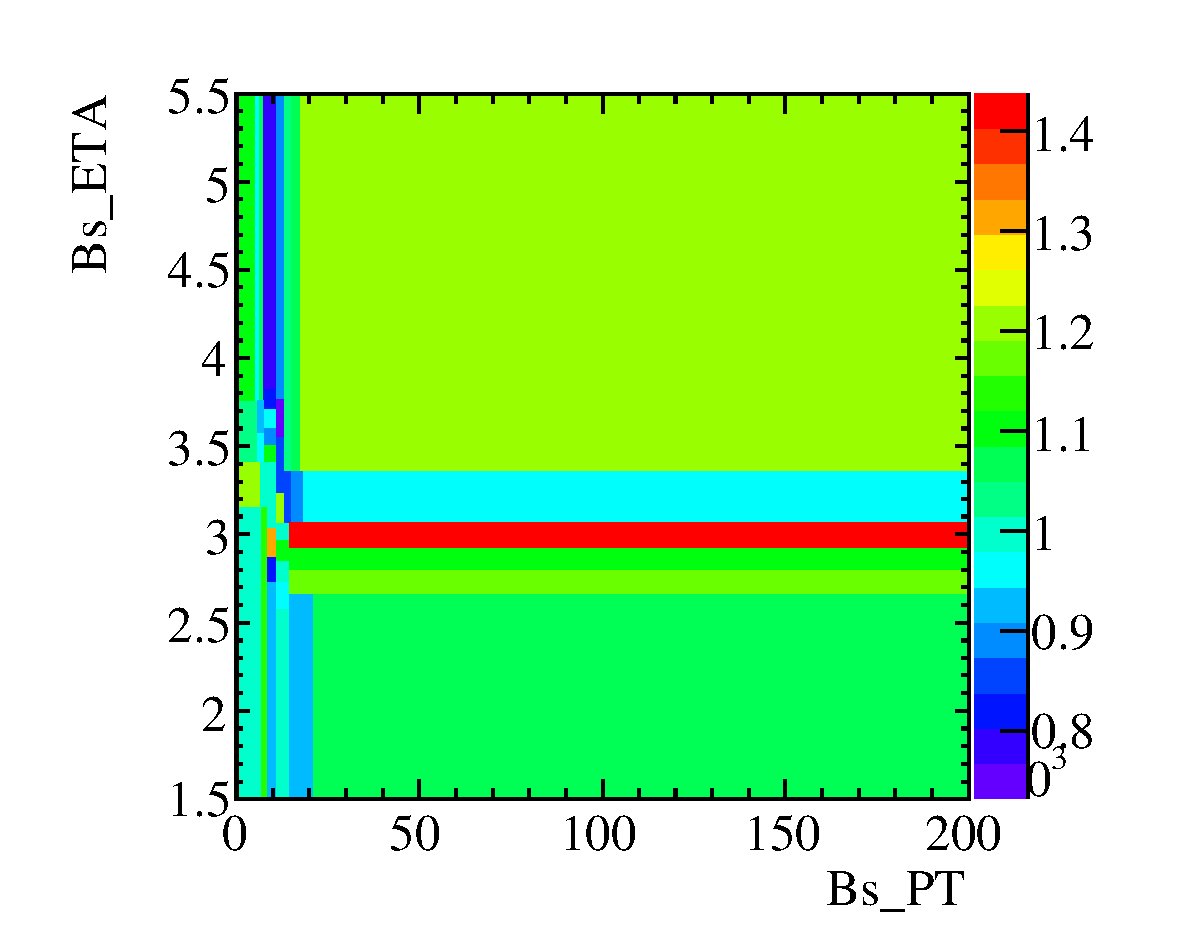
\includegraphics[height=!,width=0.45\textwidth]{figs/dataVsMC/norm_final/weights/weights_Bs_PT_Bs_ETA_Ds2KKpi_1_t0.pdf}
%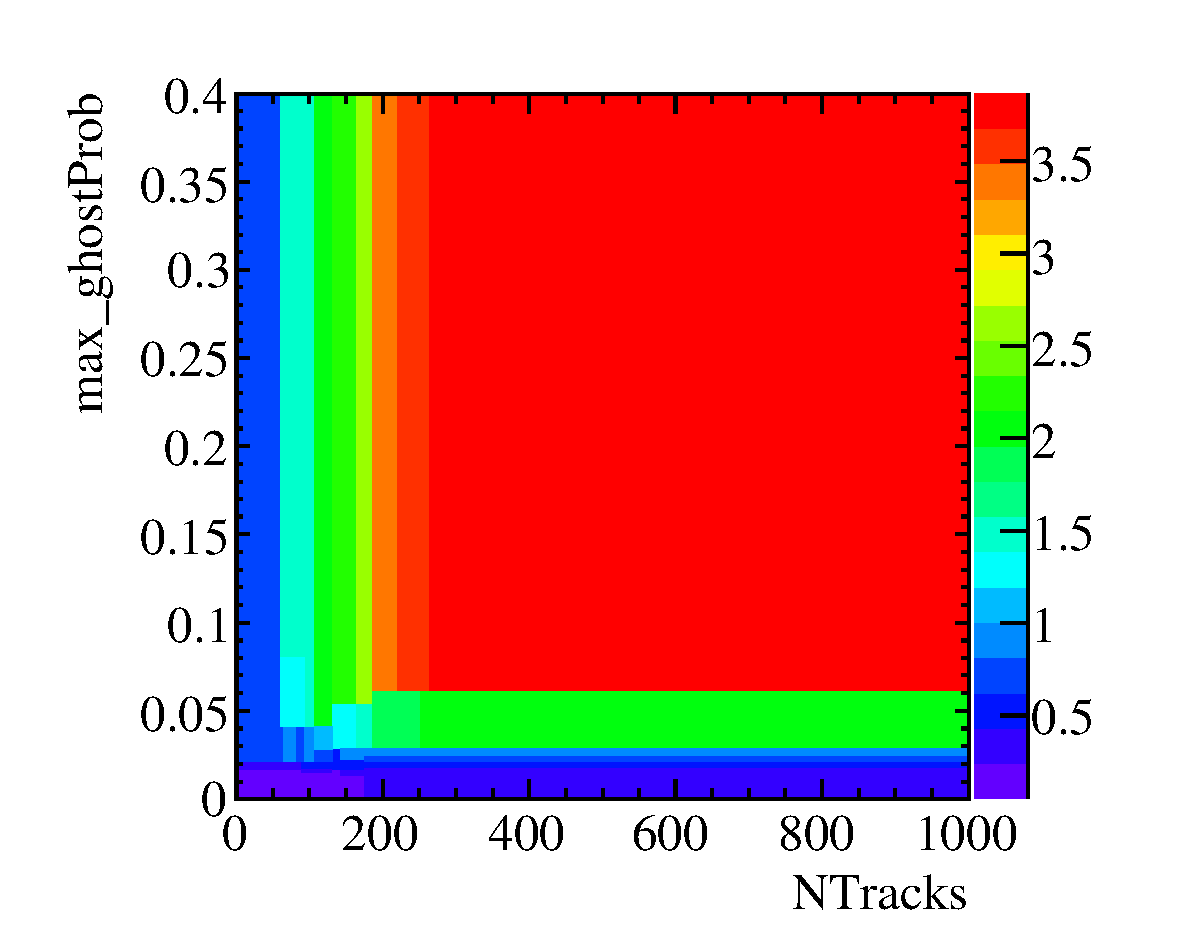
\includegraphics[height=!,width=0.45\textwidth]{figs/dataVsMC/norm_final/weights/weights_NTracks_max_ghostProb_Ds2KKpi_1_t0.pdf}
%
%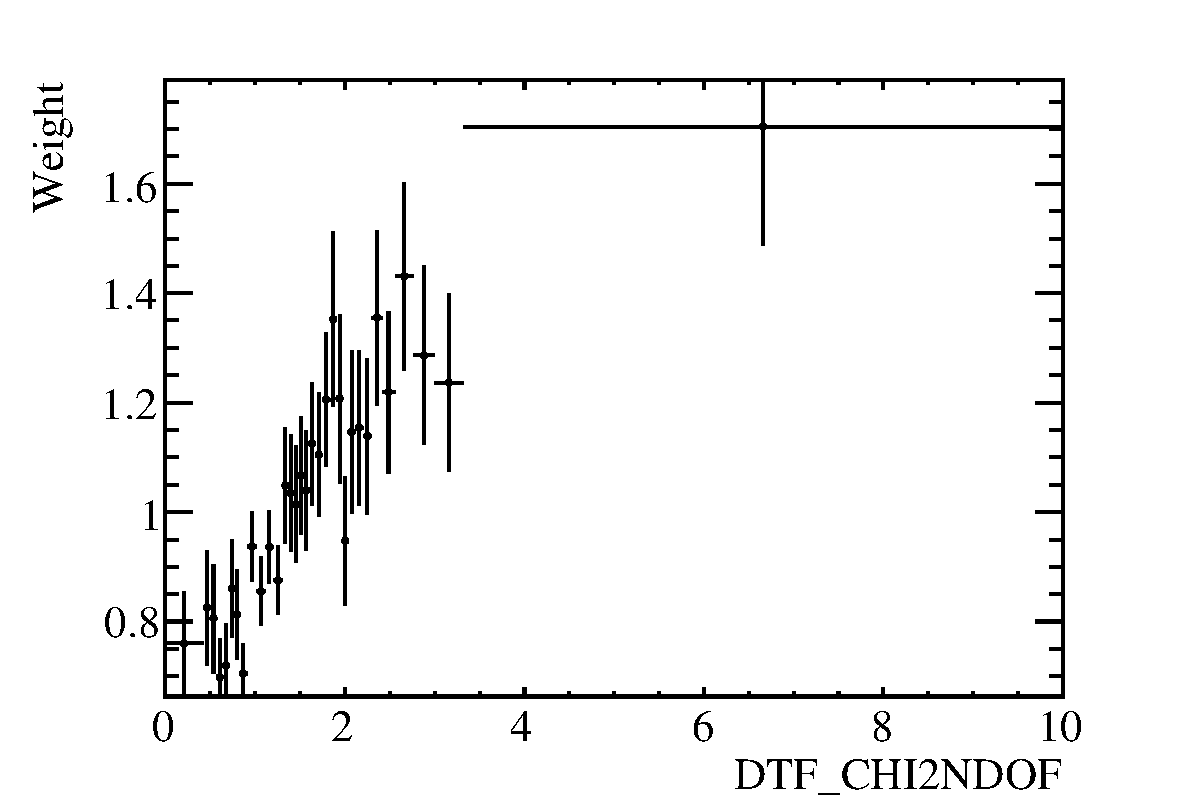
\includegraphics[height=!,width=0.45\textwidth]{figs/dataVsMC/norm_final/weights/weights_DTF_CHI2NDOF_Ds2KKpi_1_t0.pdf}
%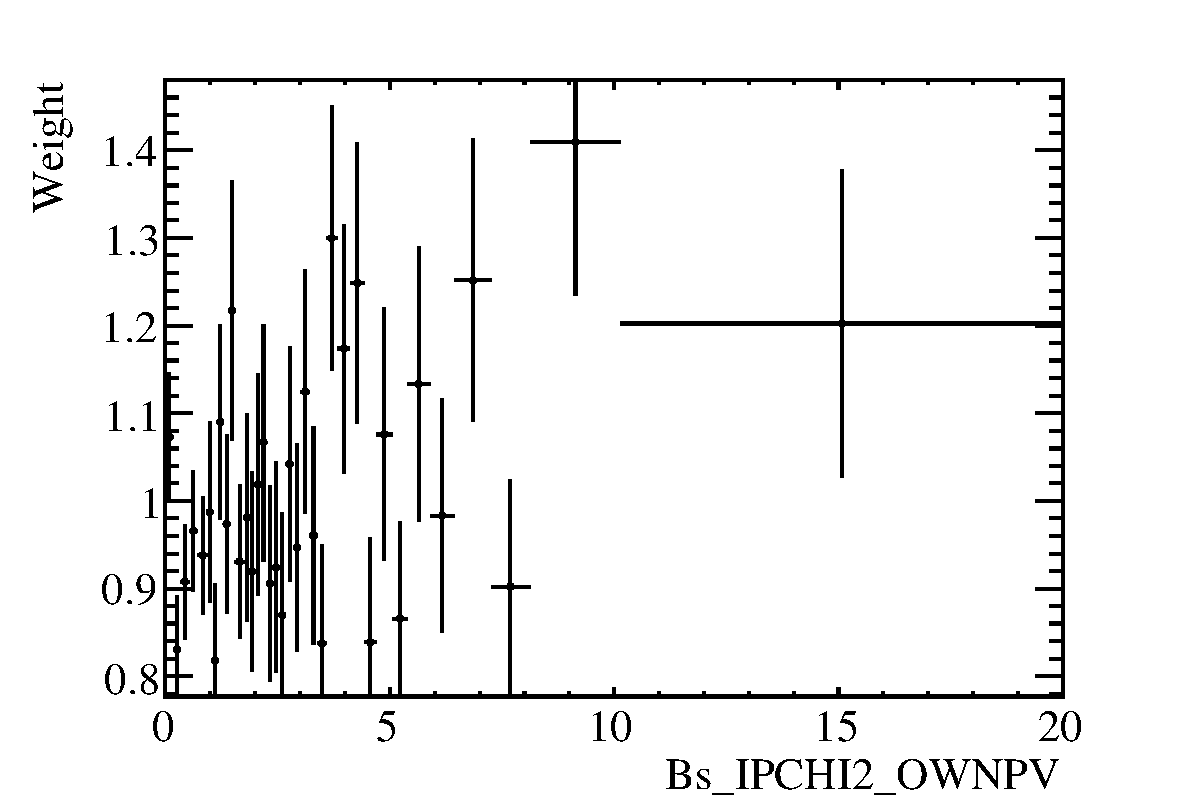
\includegraphics[height=!,width=0.45\textwidth]{figs/dataVsMC/norm_final/weights/weights_Bs_IPCHI2_OWNPV_Ds2KKpi_1_t0.pdf}
%\caption{Weights applied to correct for Data/MC differences.}
%\label{fig:}
%\end{figure}

%\begin{figure}[h]
%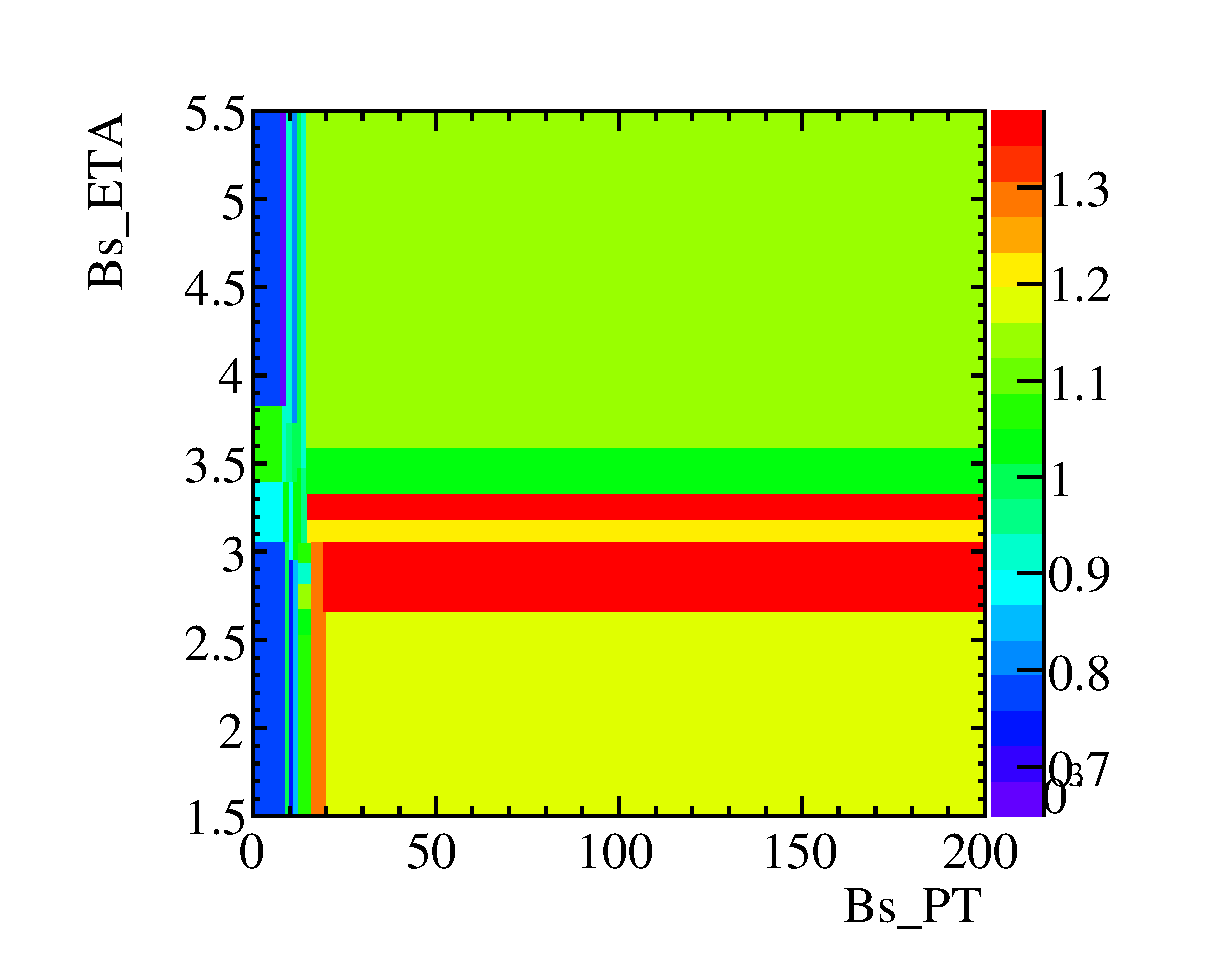
\includegraphics[height=!,width=0.45\textwidth]{figs/dataVsMC/norm_final/weights/weights_Bs_PT_Bs_ETA_Ds2KKpi_1_t1.eps}
%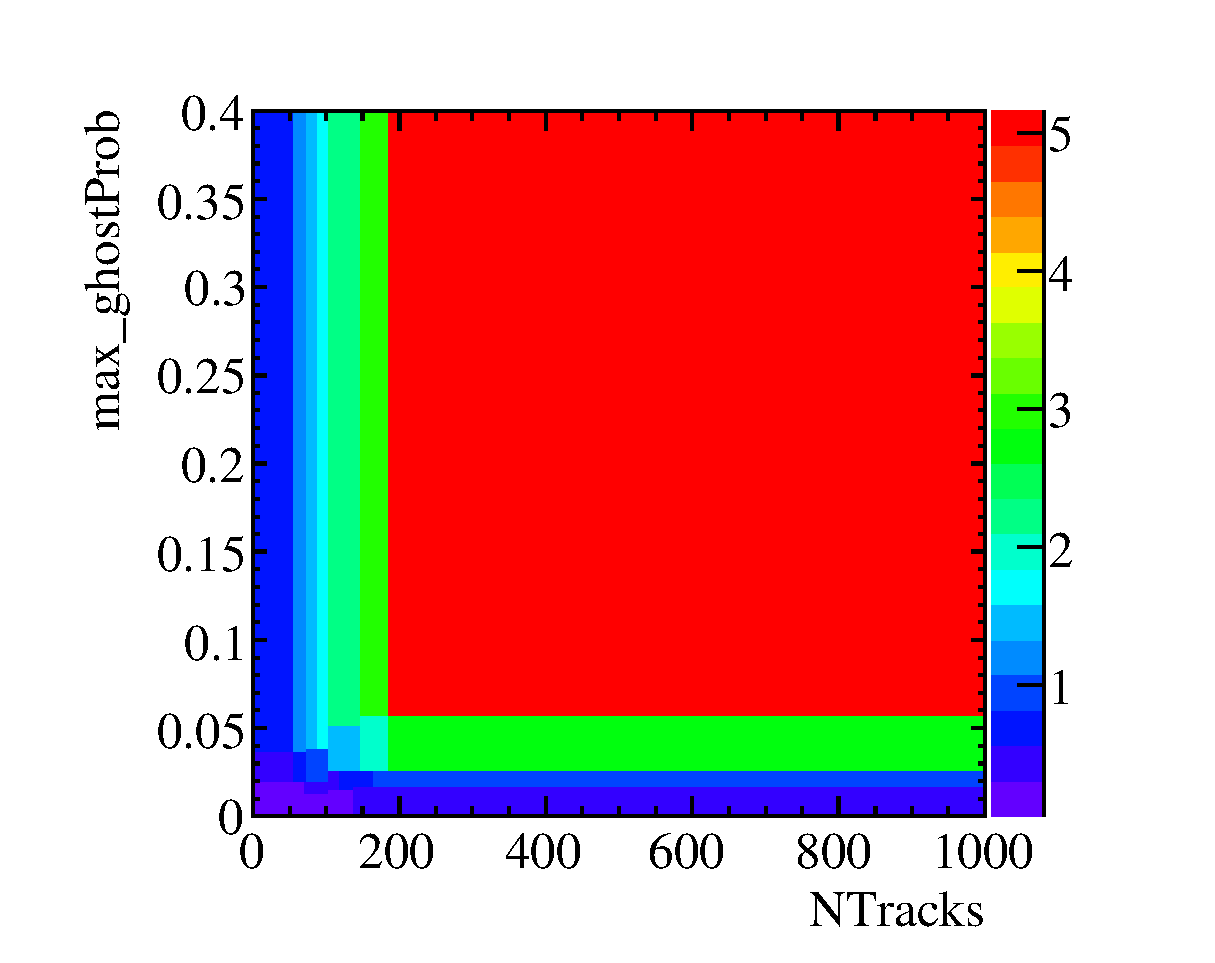
\includegraphics[height=!,width=0.45\textwidth]{figs/dataVsMC/norm_final/weights/weights_NTracks_max_ghostProb_Ds2KKpi_1_t1.eps}
%
%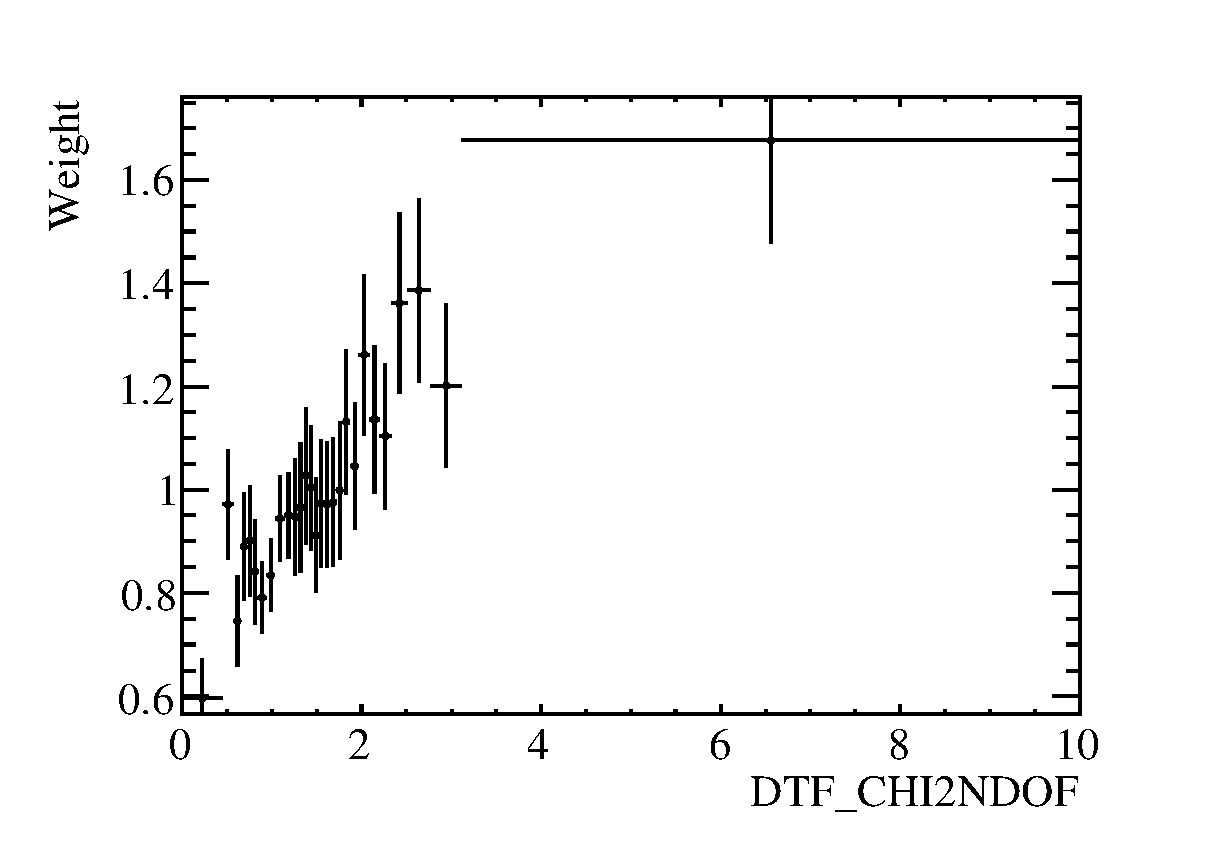
\includegraphics[height=!,width=0.45\textwidth]{figs/dataVsMC/norm_final/weights/weights_DTF_CHI2NDOF_Ds2KKpi_1_t1.eps}
%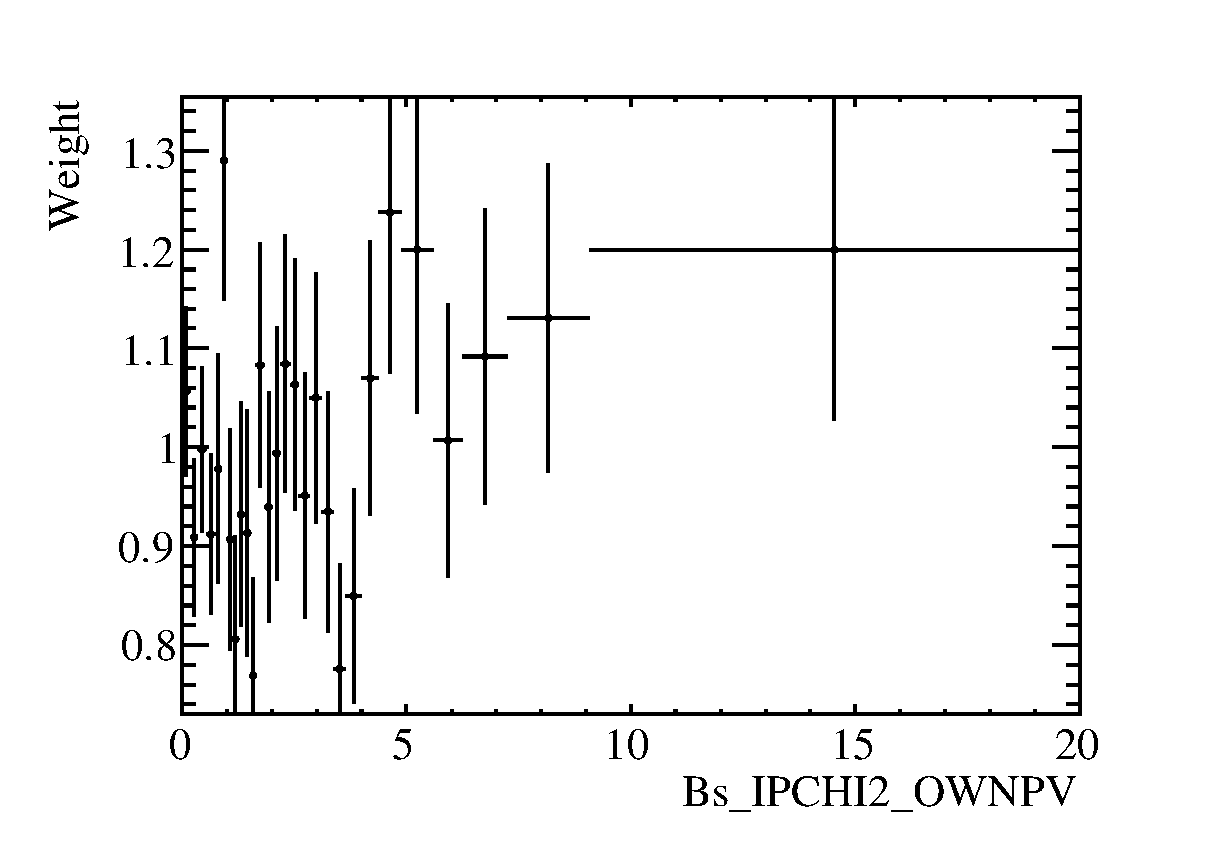
\includegraphics[height=!,width=0.45\textwidth]{figs/dataVsMC/norm_final/weights/weights_Bs_IPCHI2_OWNPV_Ds2KKpi_1_t1.eps}
%\caption{}
%\label{fig:}
%\end{figure}


\begin{figure}[h]
\centering
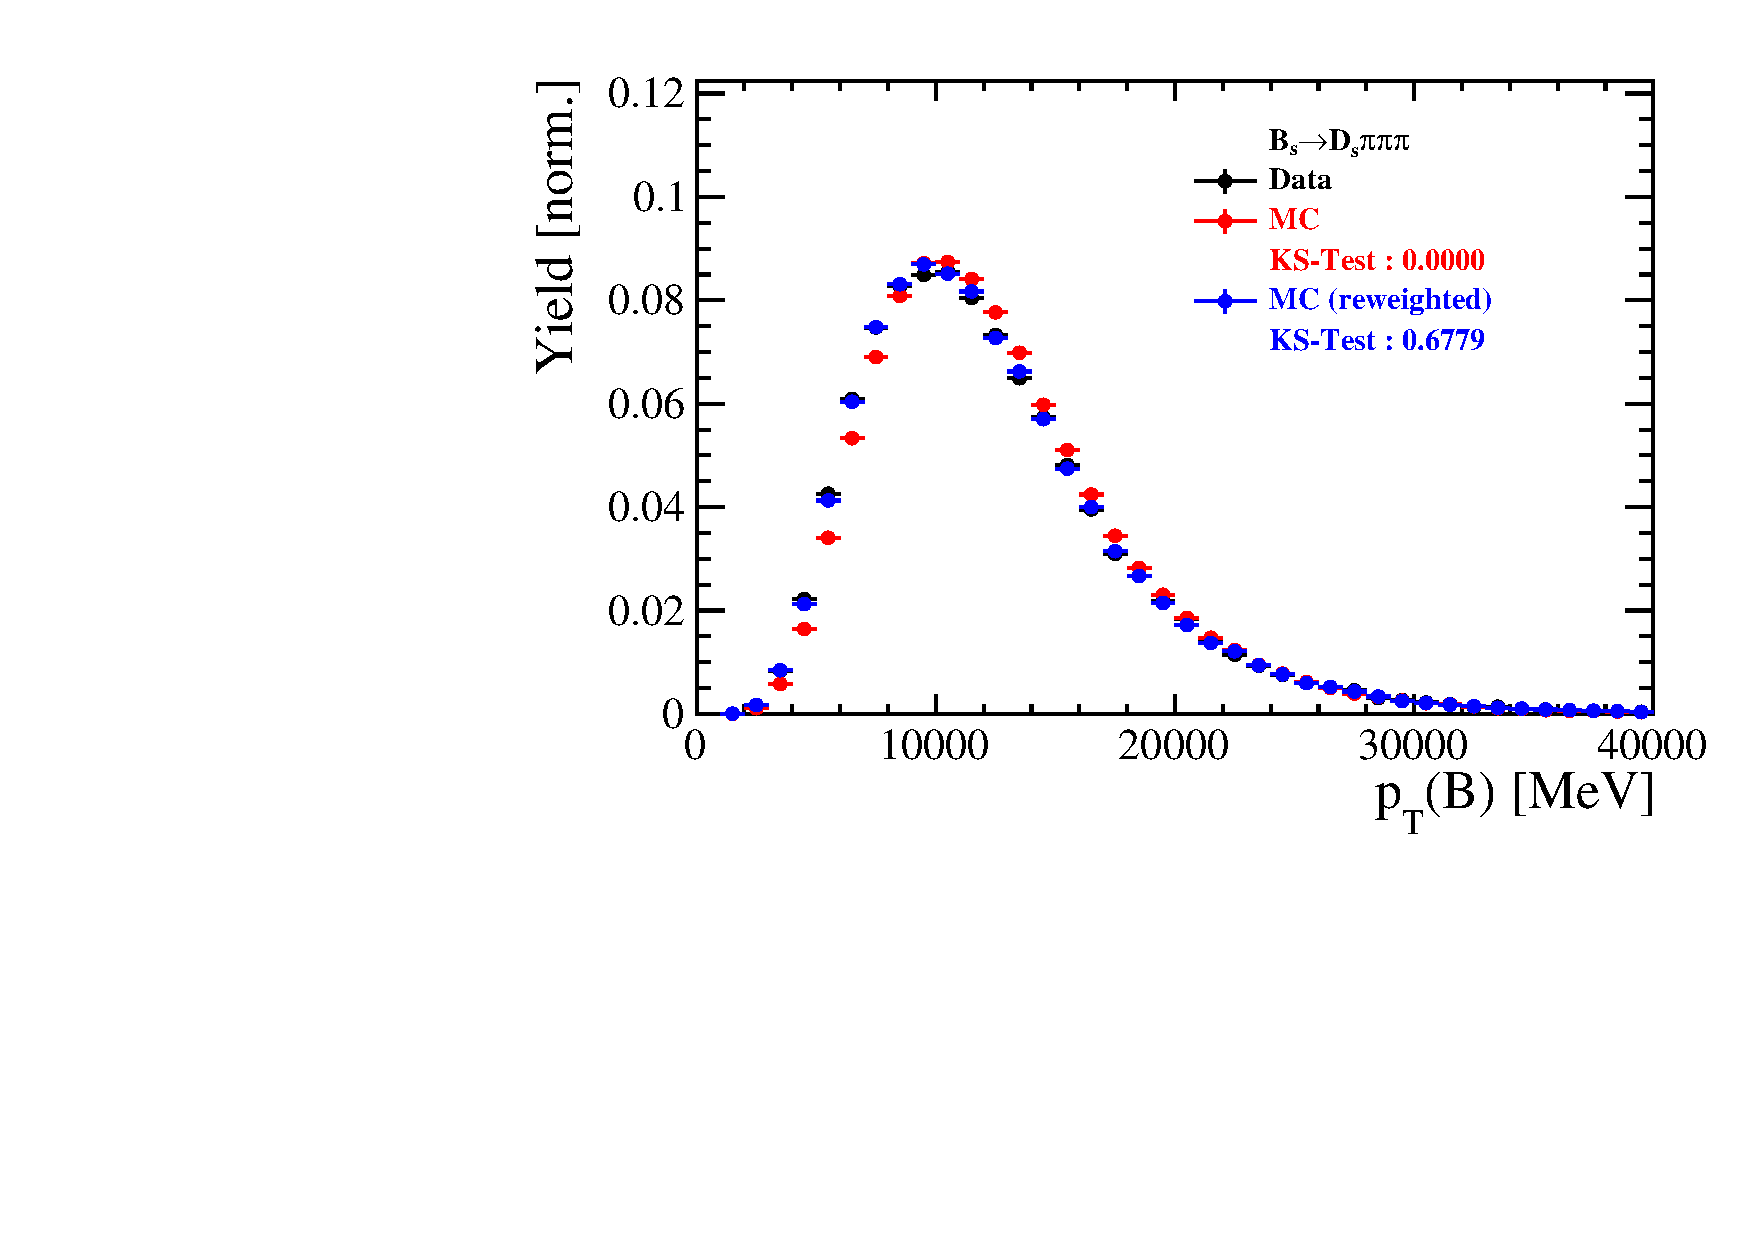
\includegraphics[height=!,width=0.3\textwidth]{figs/dataVsMC/norm_final/Ds2all_Bs_PT.pdf}
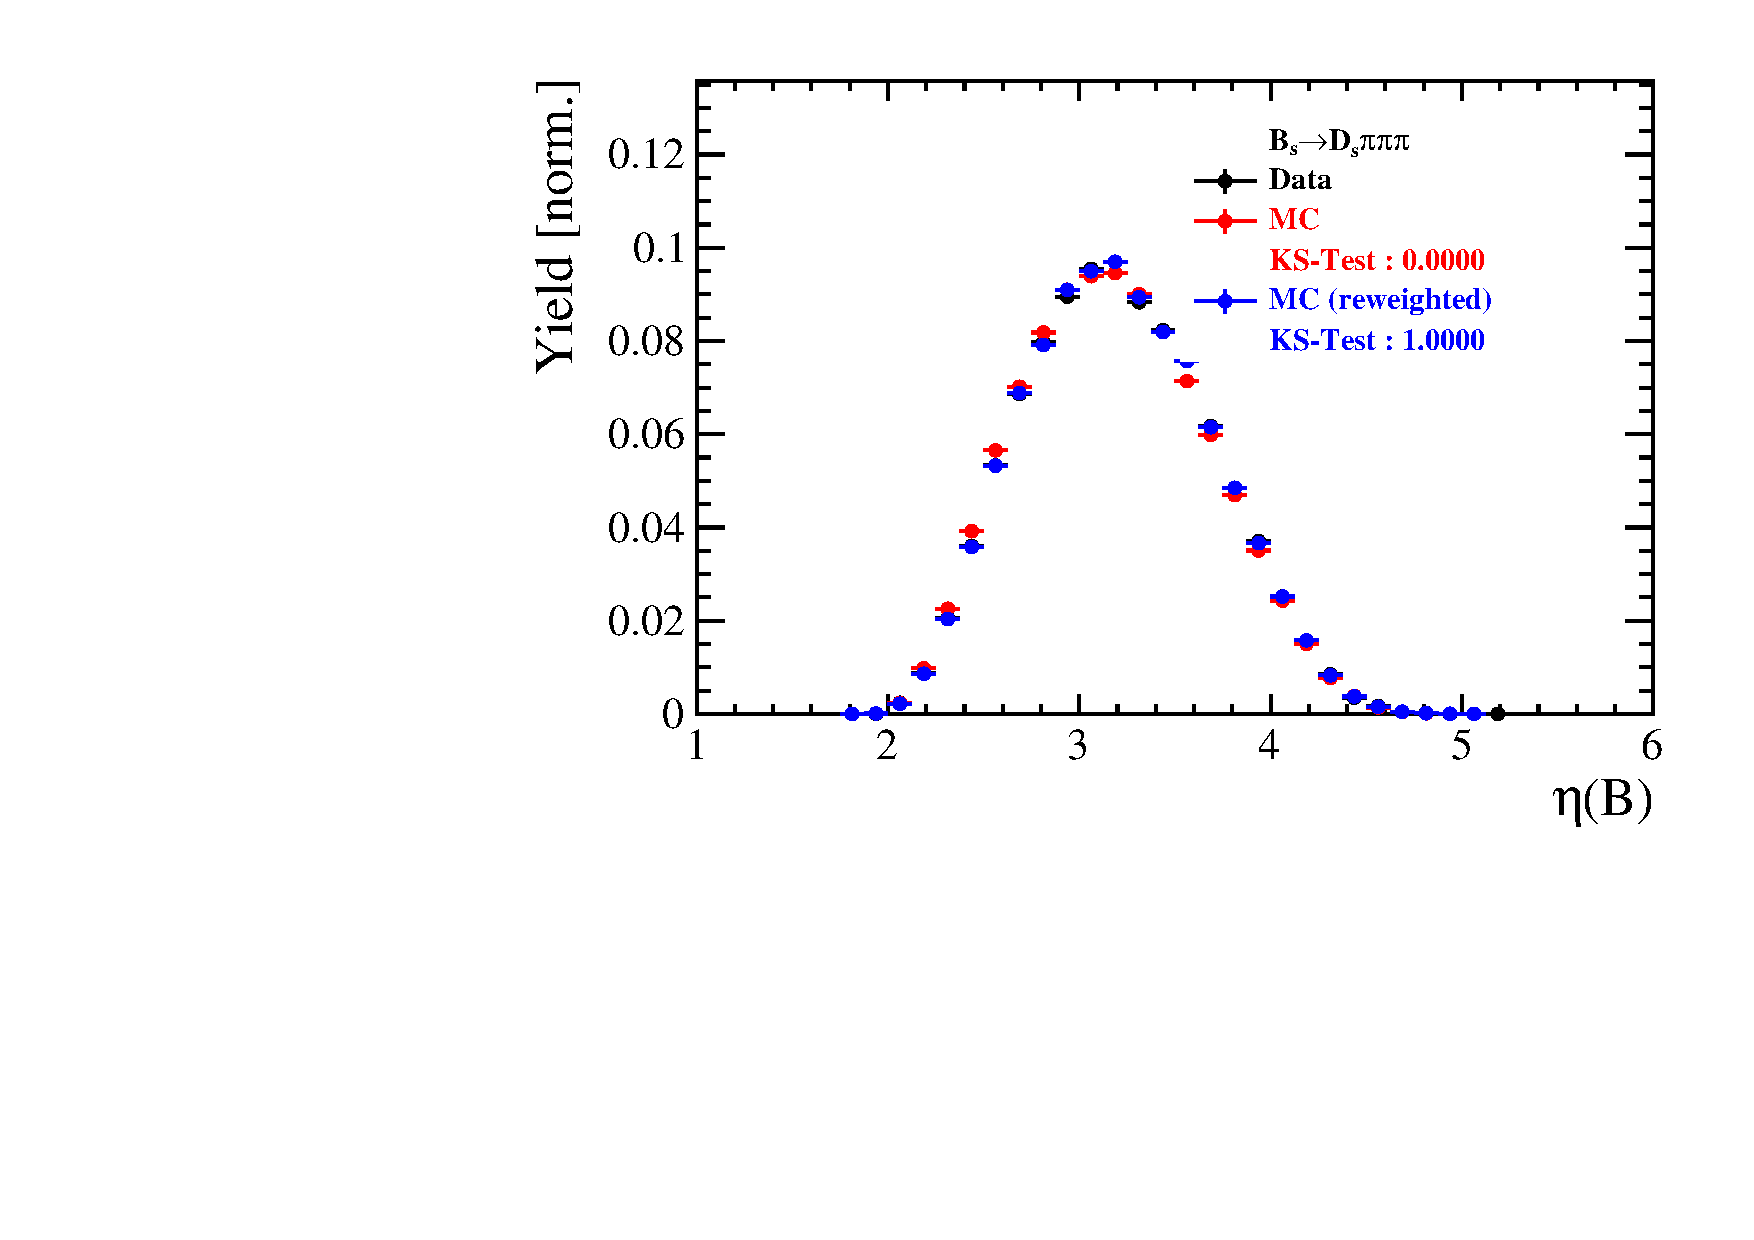
\includegraphics[height=!,width=0.3\textwidth]{figs/dataVsMC/norm_final/Ds2all_Bs_ETA.pdf}
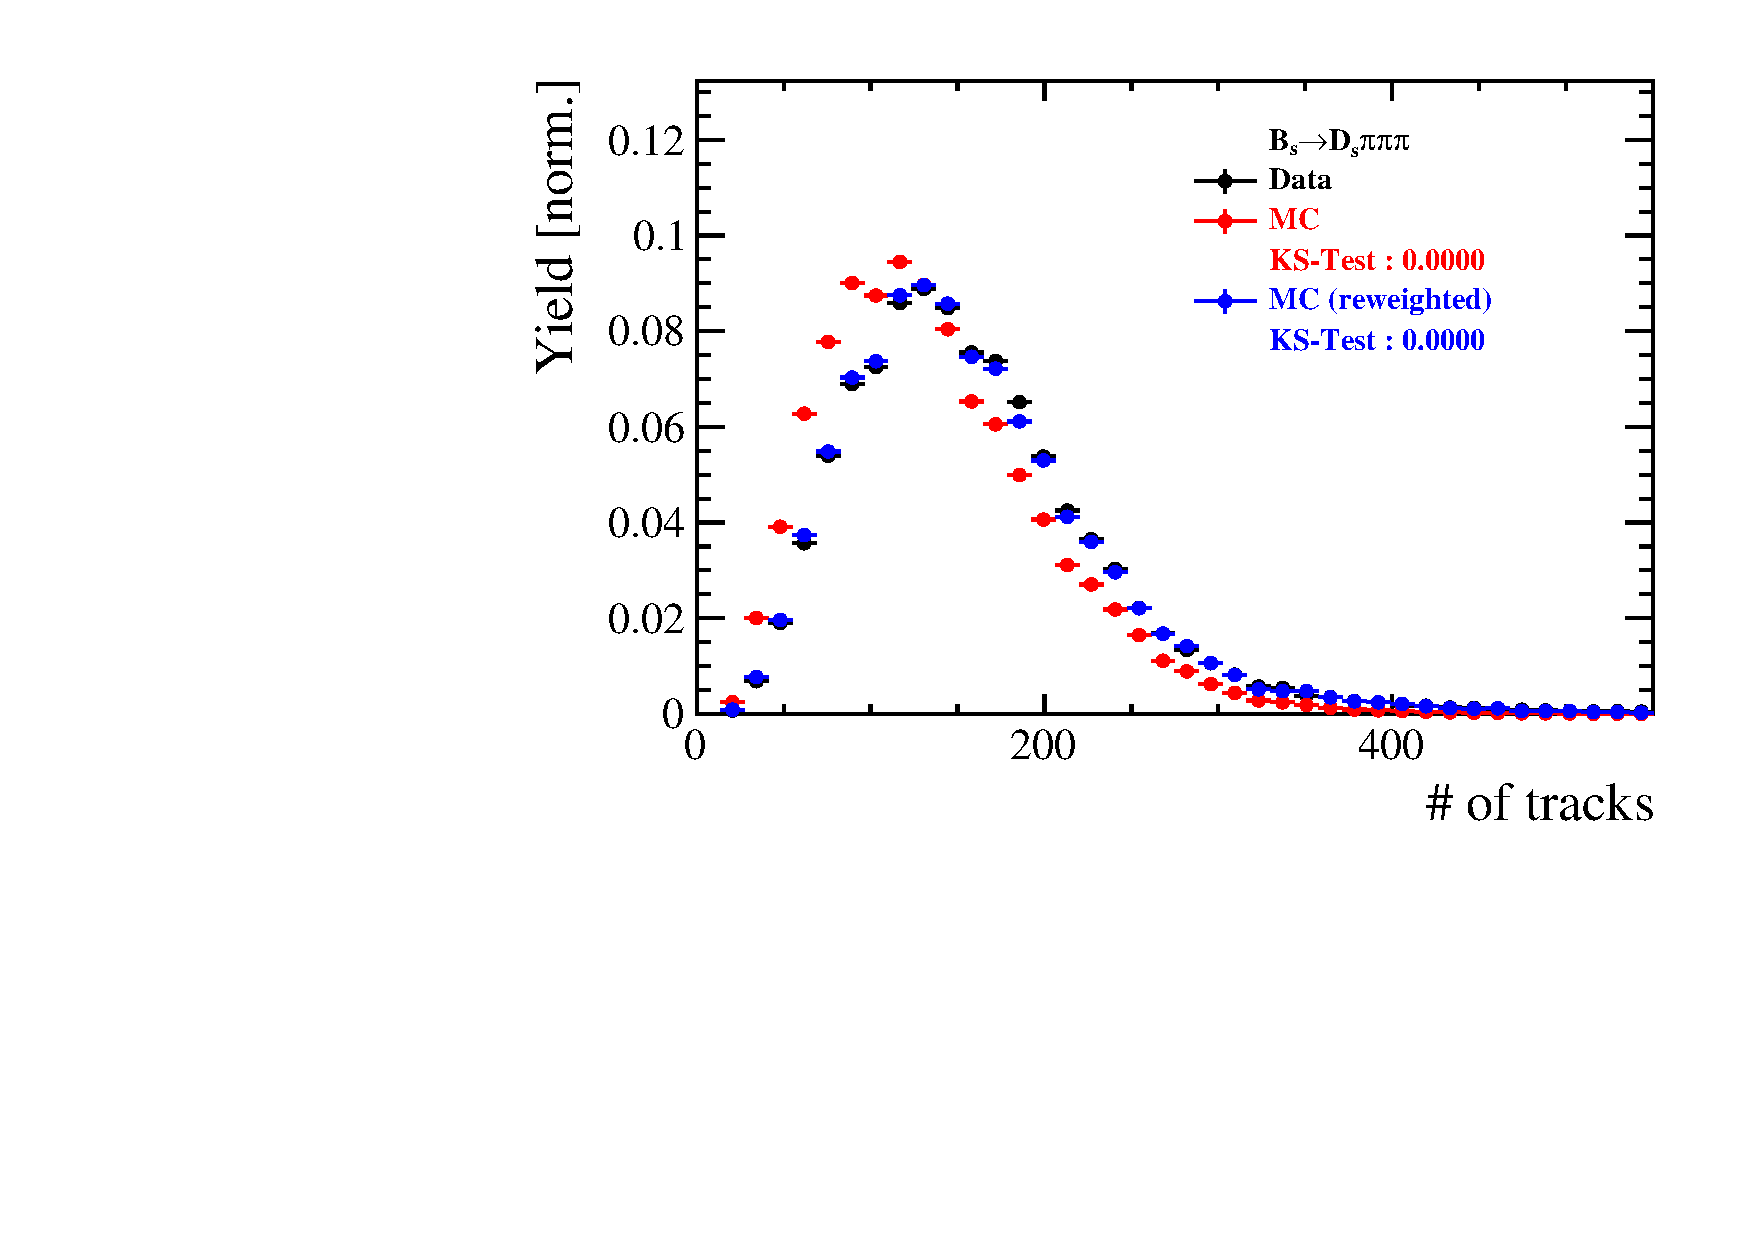
\includegraphics[height=!,width=0.3\textwidth]{figs/dataVsMC/norm_final/Ds2all_NTracks.pdf}

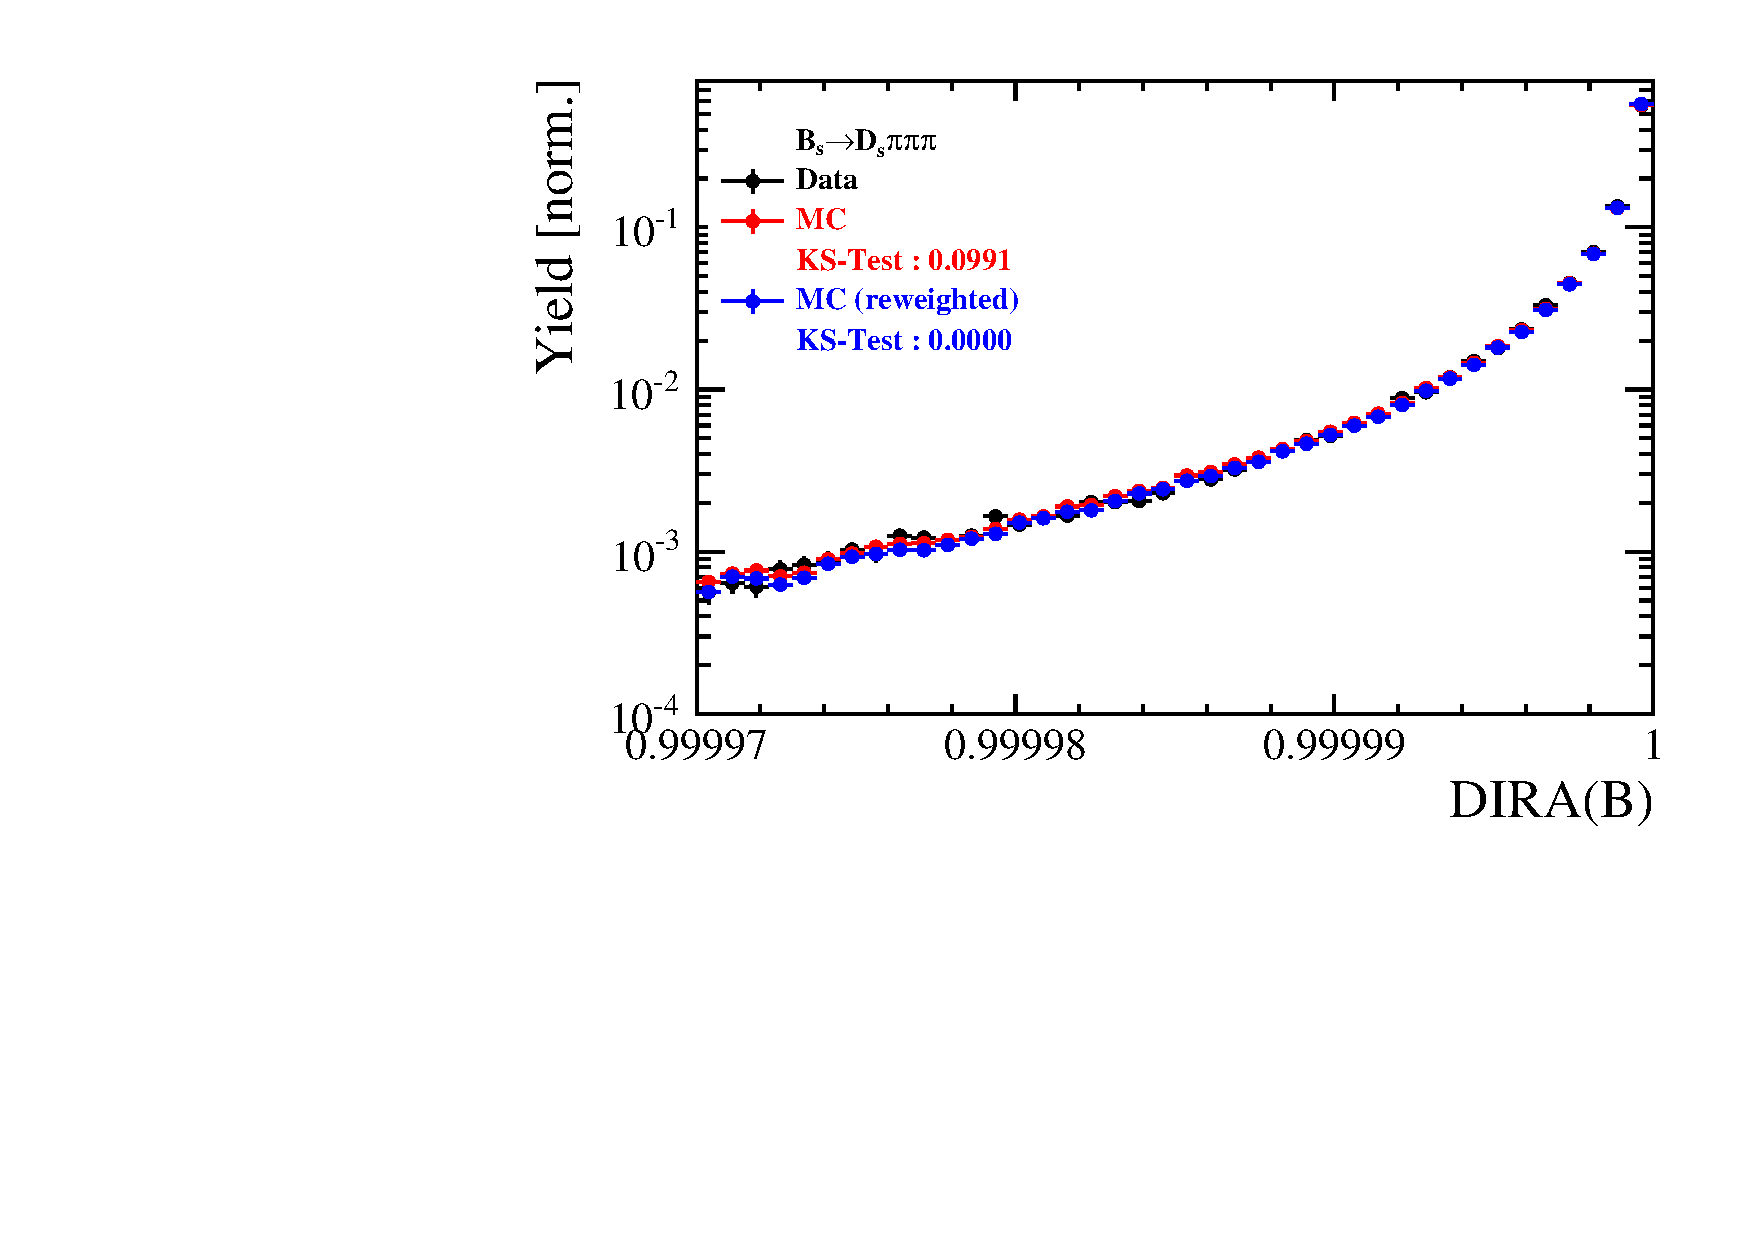
\includegraphics[height=!,width=0.3\textwidth]{figs/dataVsMC/norm_final/Ds2all_Bs_DIRA_OWNPV.pdf}
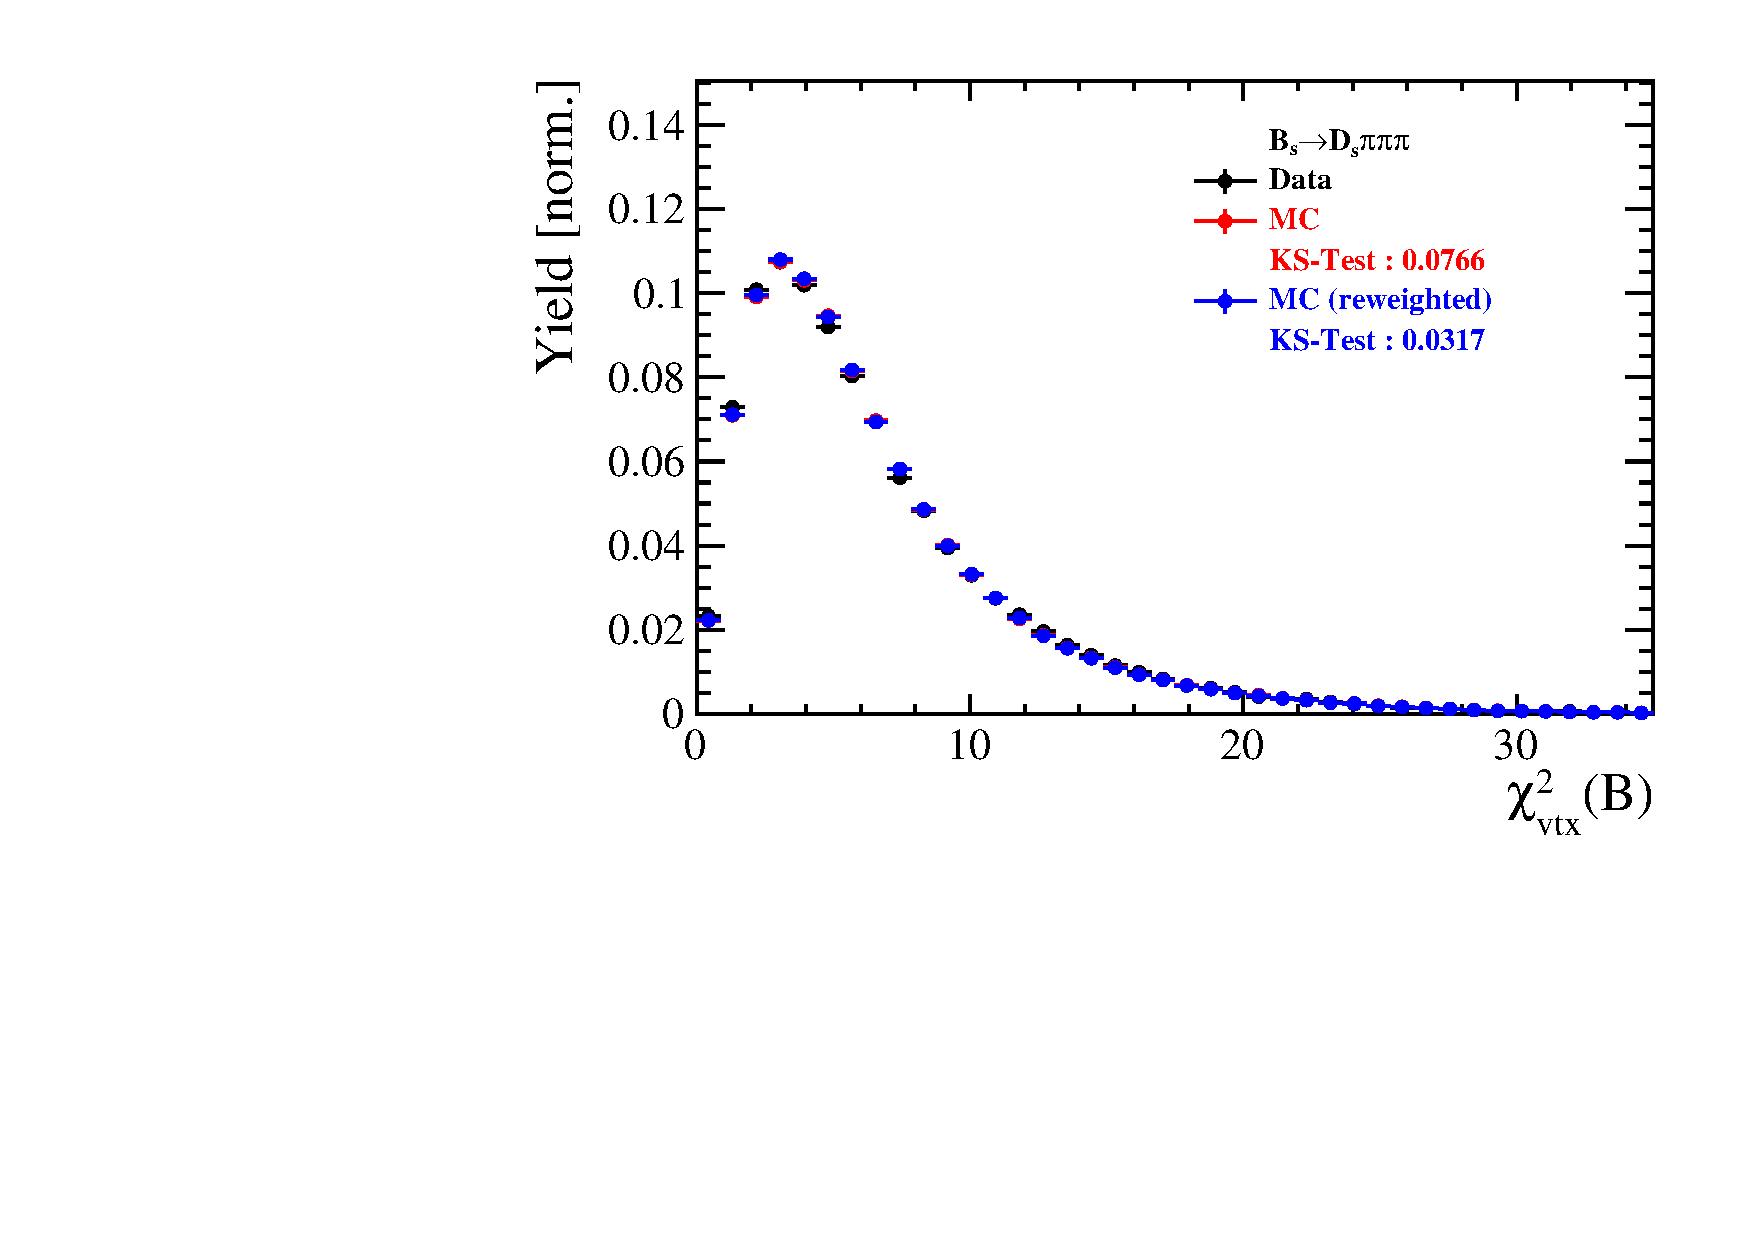
\includegraphics[height=!,width=0.3\textwidth]{figs/dataVsMC/norm_final/Ds2all_Bs_ENDVERTEX_CHI2.pdf}
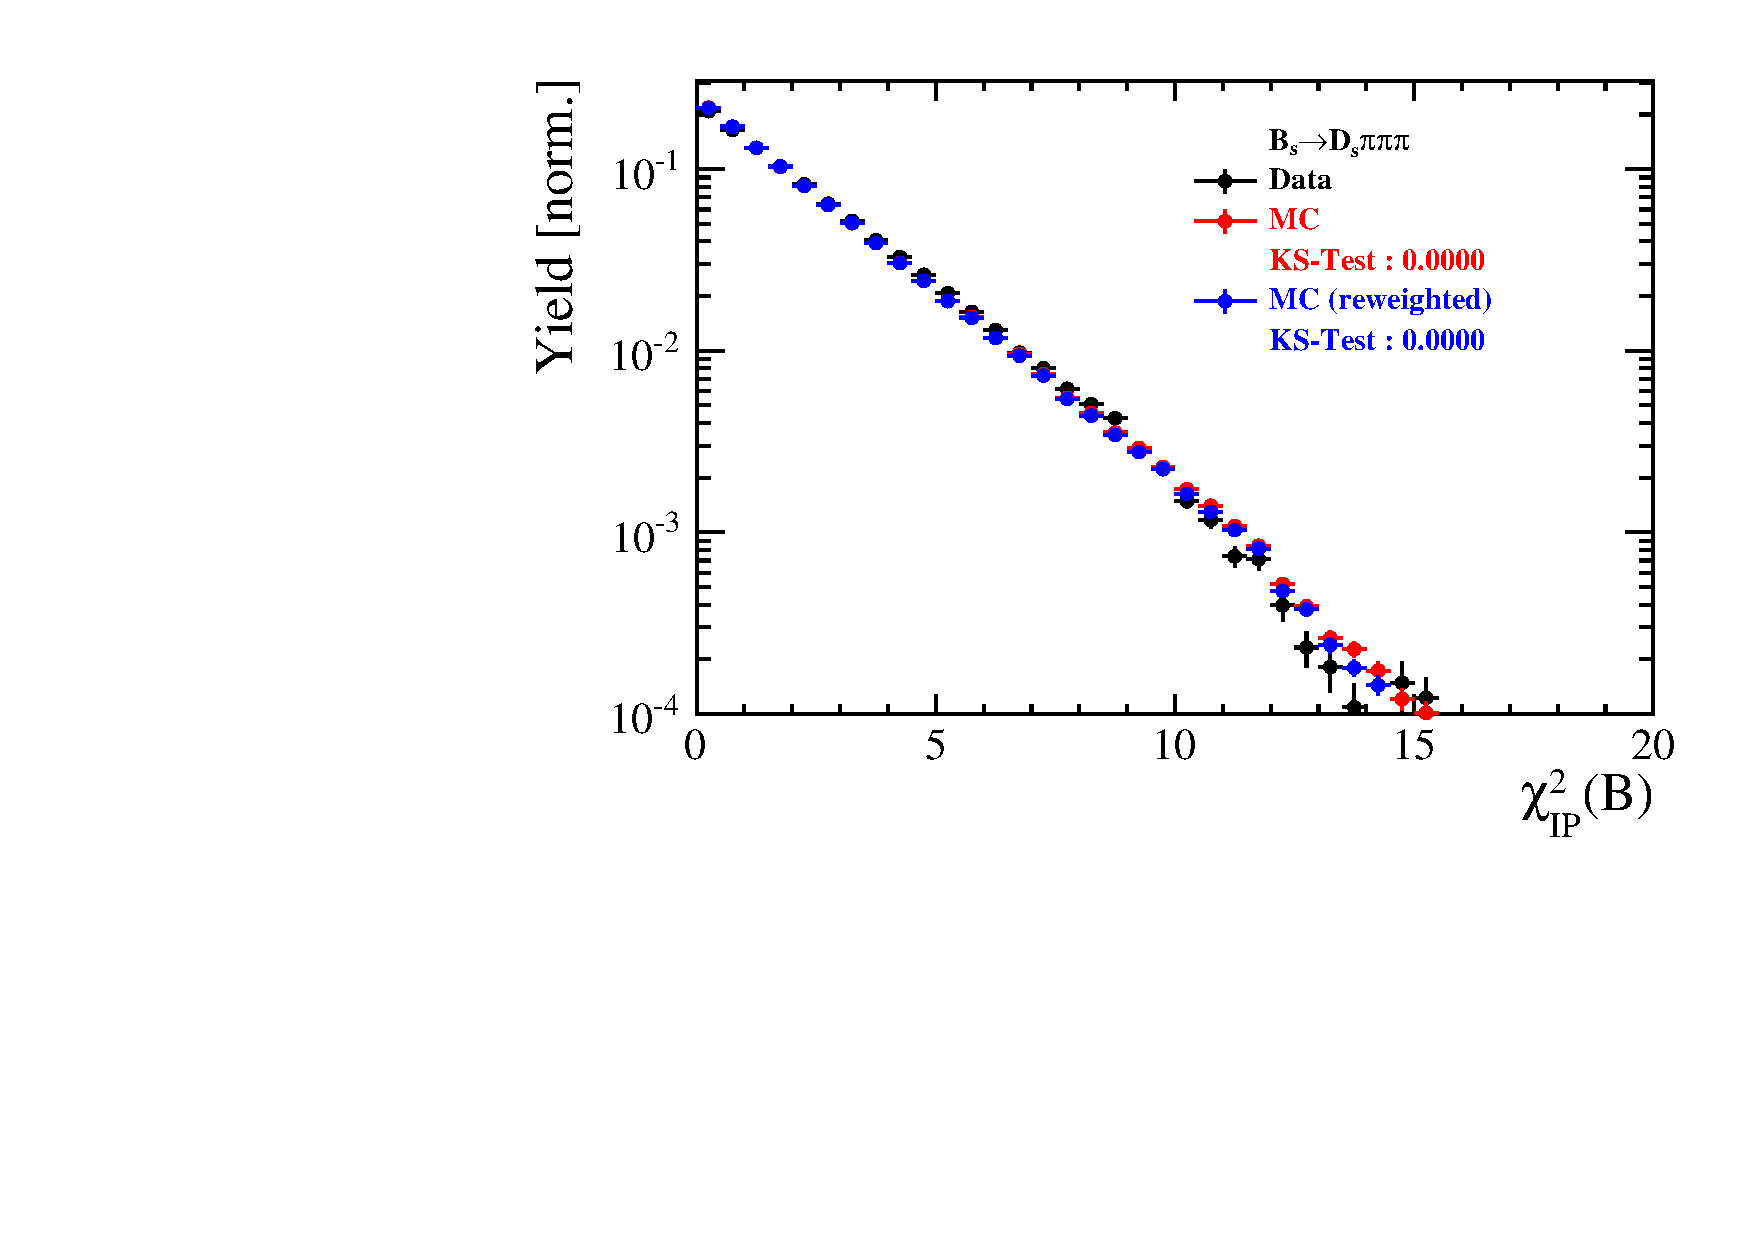
\includegraphics[height=!,width=0.3\textwidth]{figs/dataVsMC/norm_final/Ds2all_Bs_IPCHI2_OWNPV.pdf}

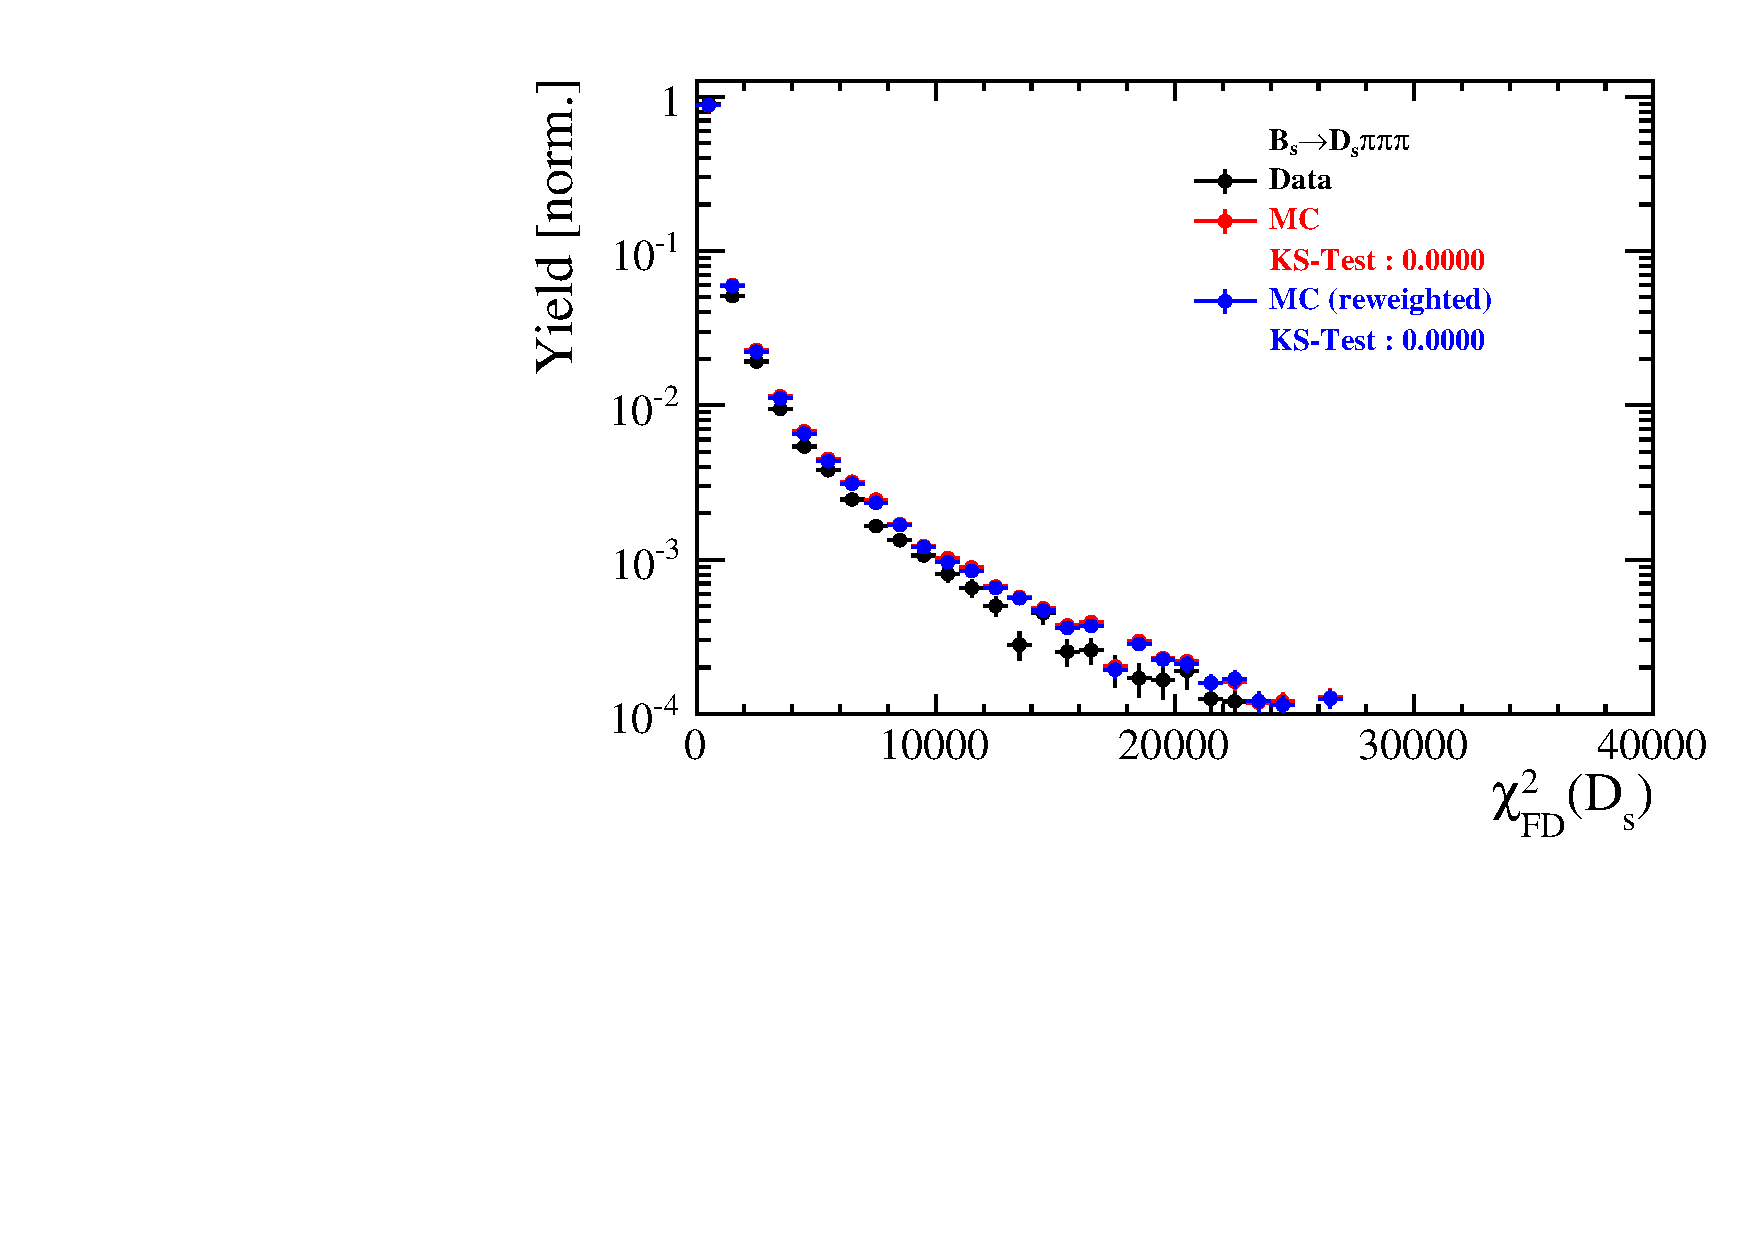
\includegraphics[height=!,width=0.3\textwidth]{figs/dataVsMC/norm_final/Ds2all_Ds_FDCHI2_ORIVX.pdf}
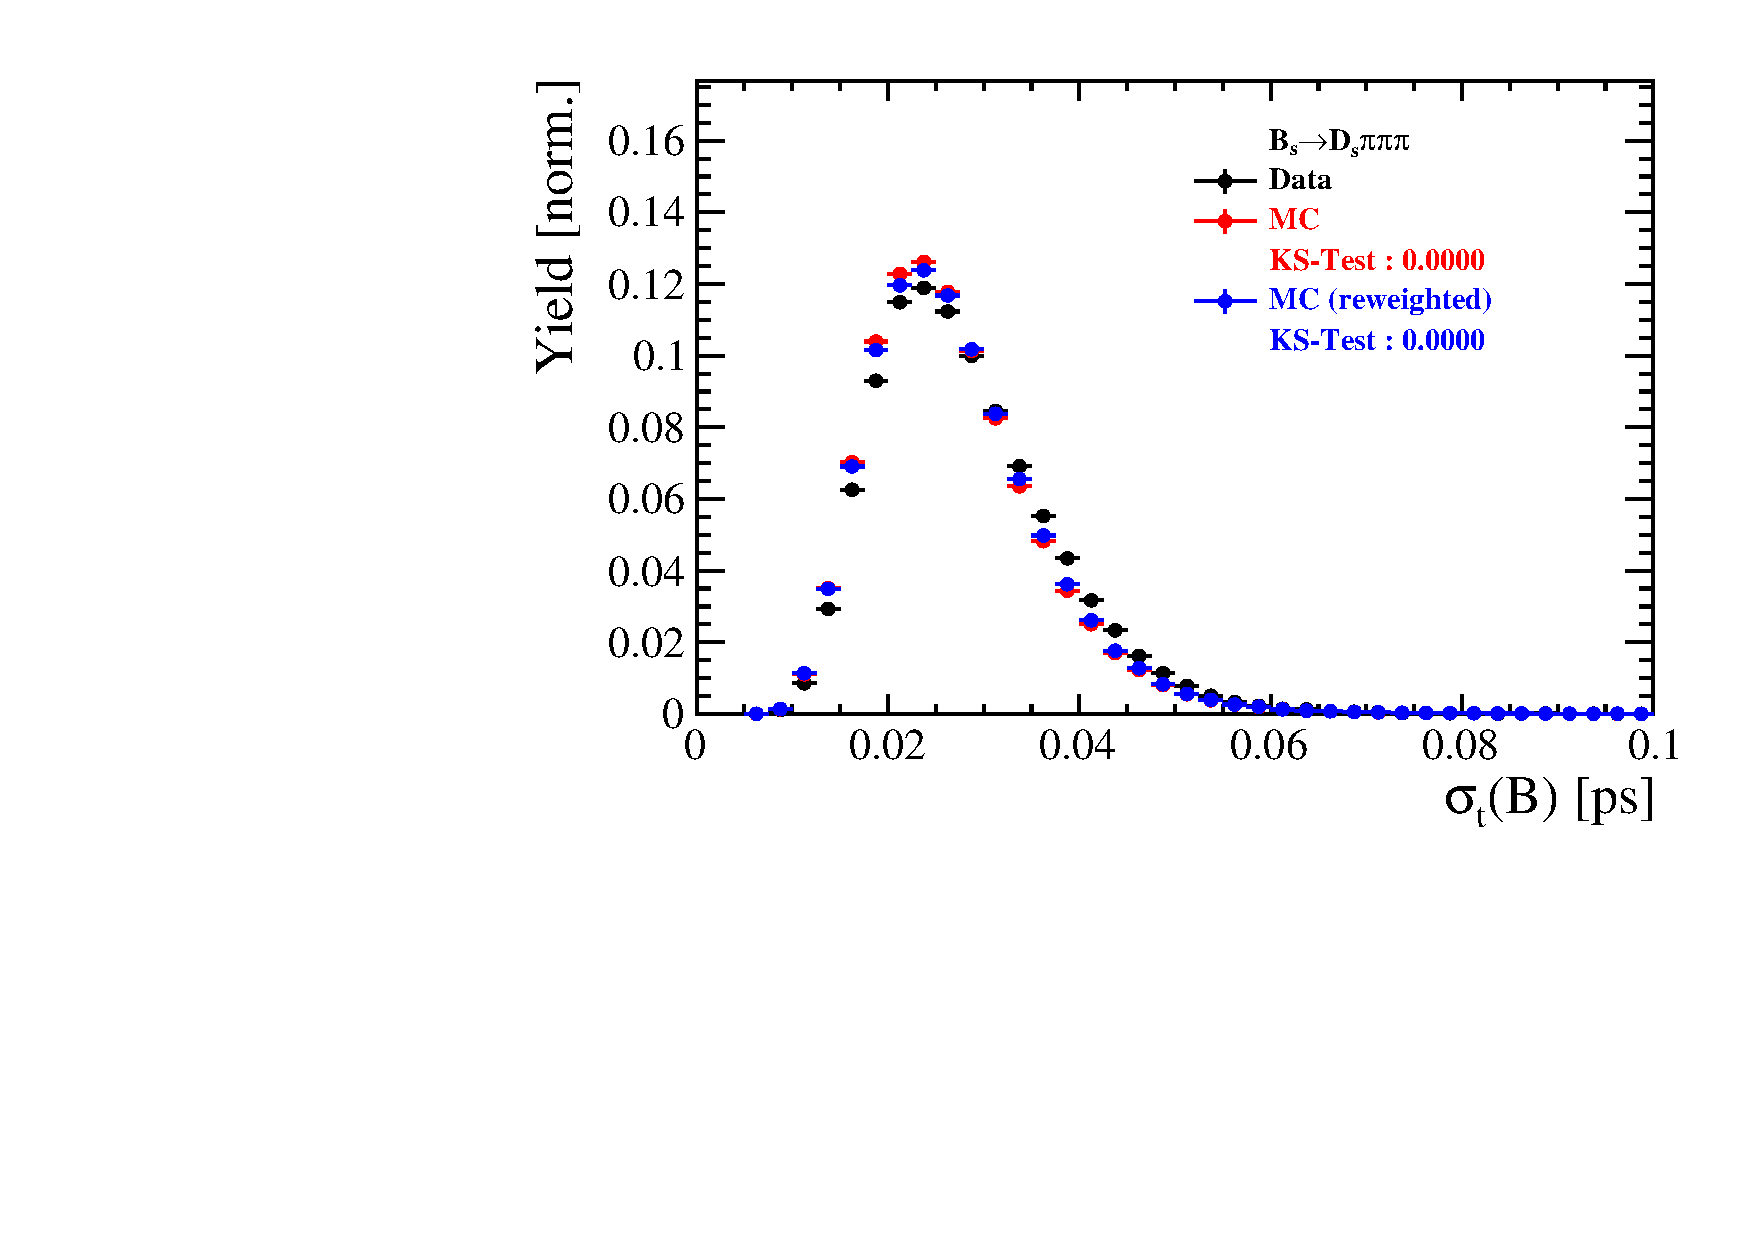
\includegraphics[height=!,width=0.3\textwidth]{figs/dataVsMC/norm_final/Ds2all_Bs_BsDTF_TAUERR.pdf}
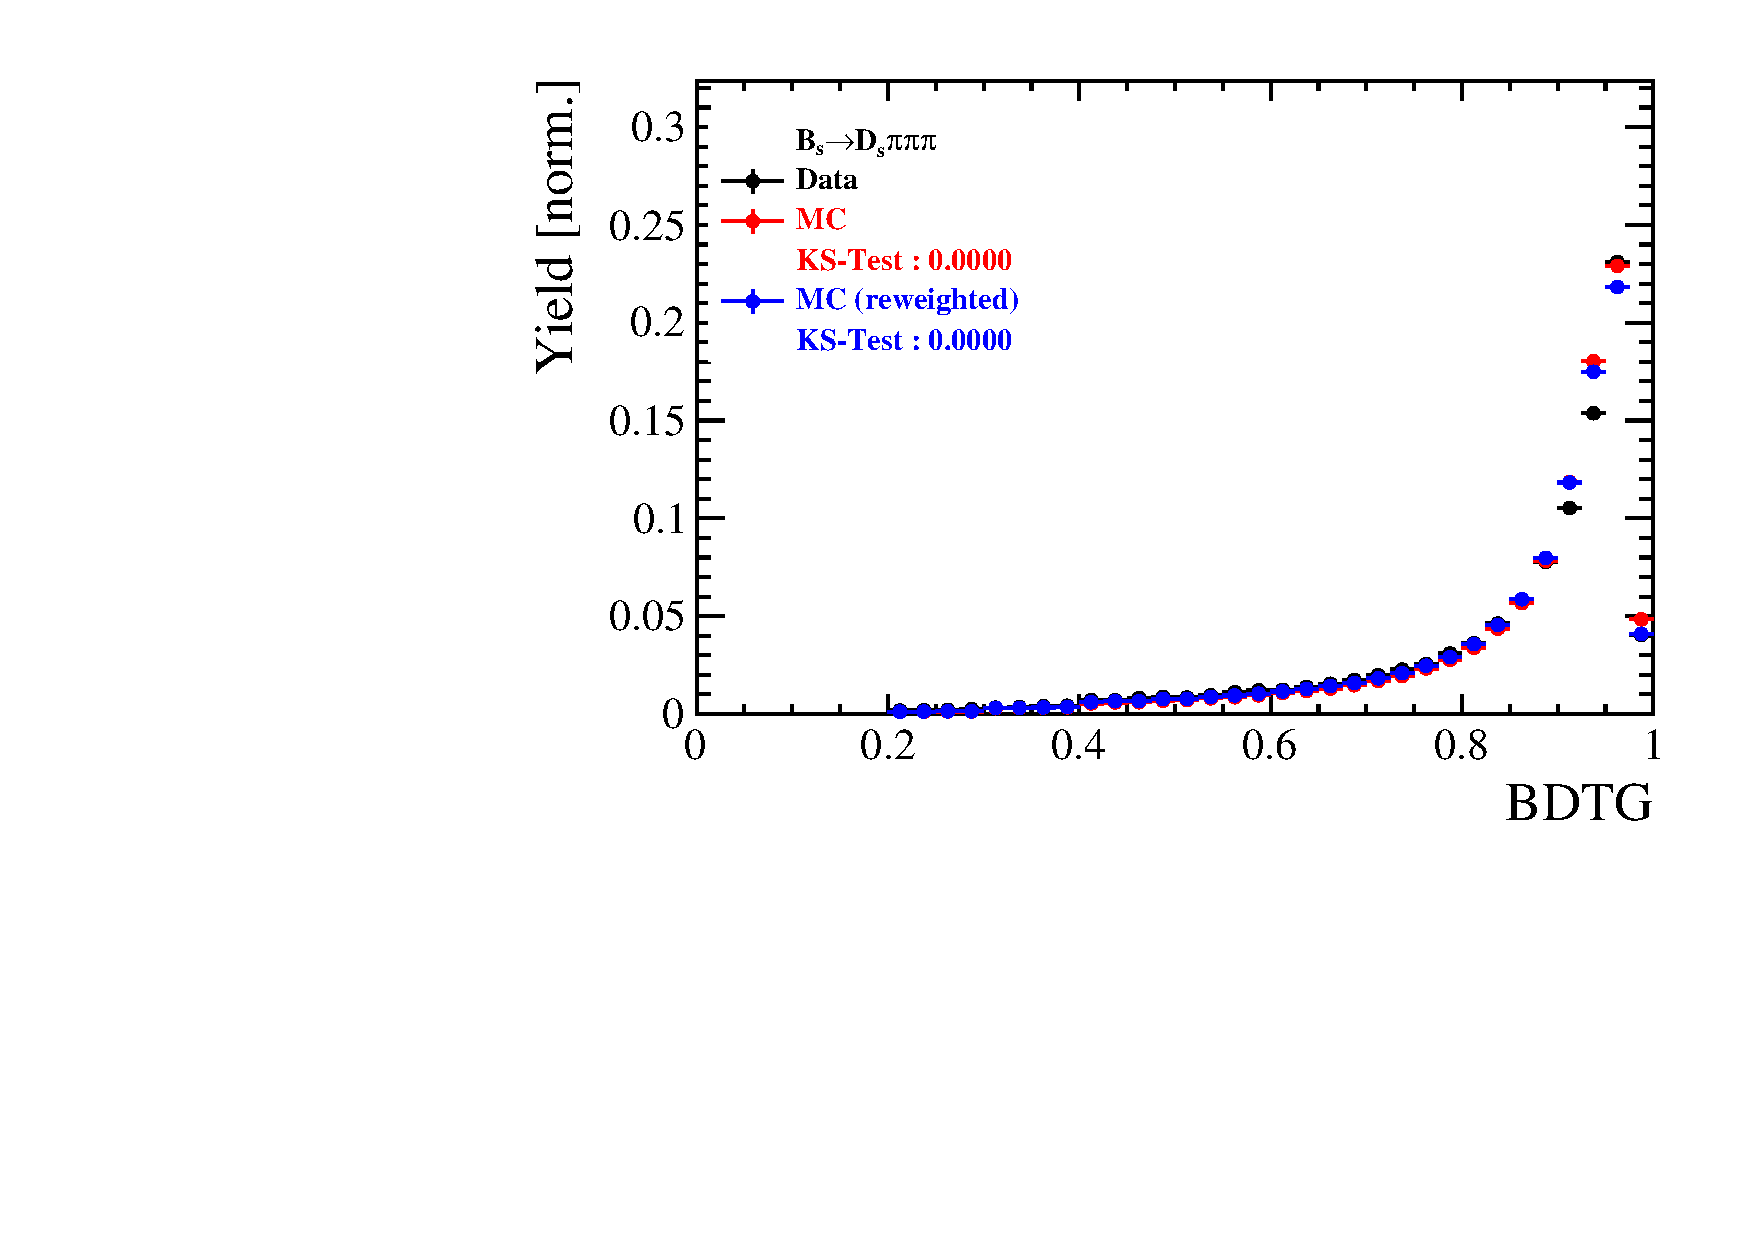
\includegraphics[height=!,width=0.3\textwidth]{figs/dataVsMC/norm_final/Ds2all_BDTG_response.pdf}


\caption{\footnotesize Comparison between data and MC of selected variables for $B_s\to D_s\pi\pi\pi$ decays.}
\label{fig:}
%\end{figure}

%\begin{figure}[h]
%\centering
%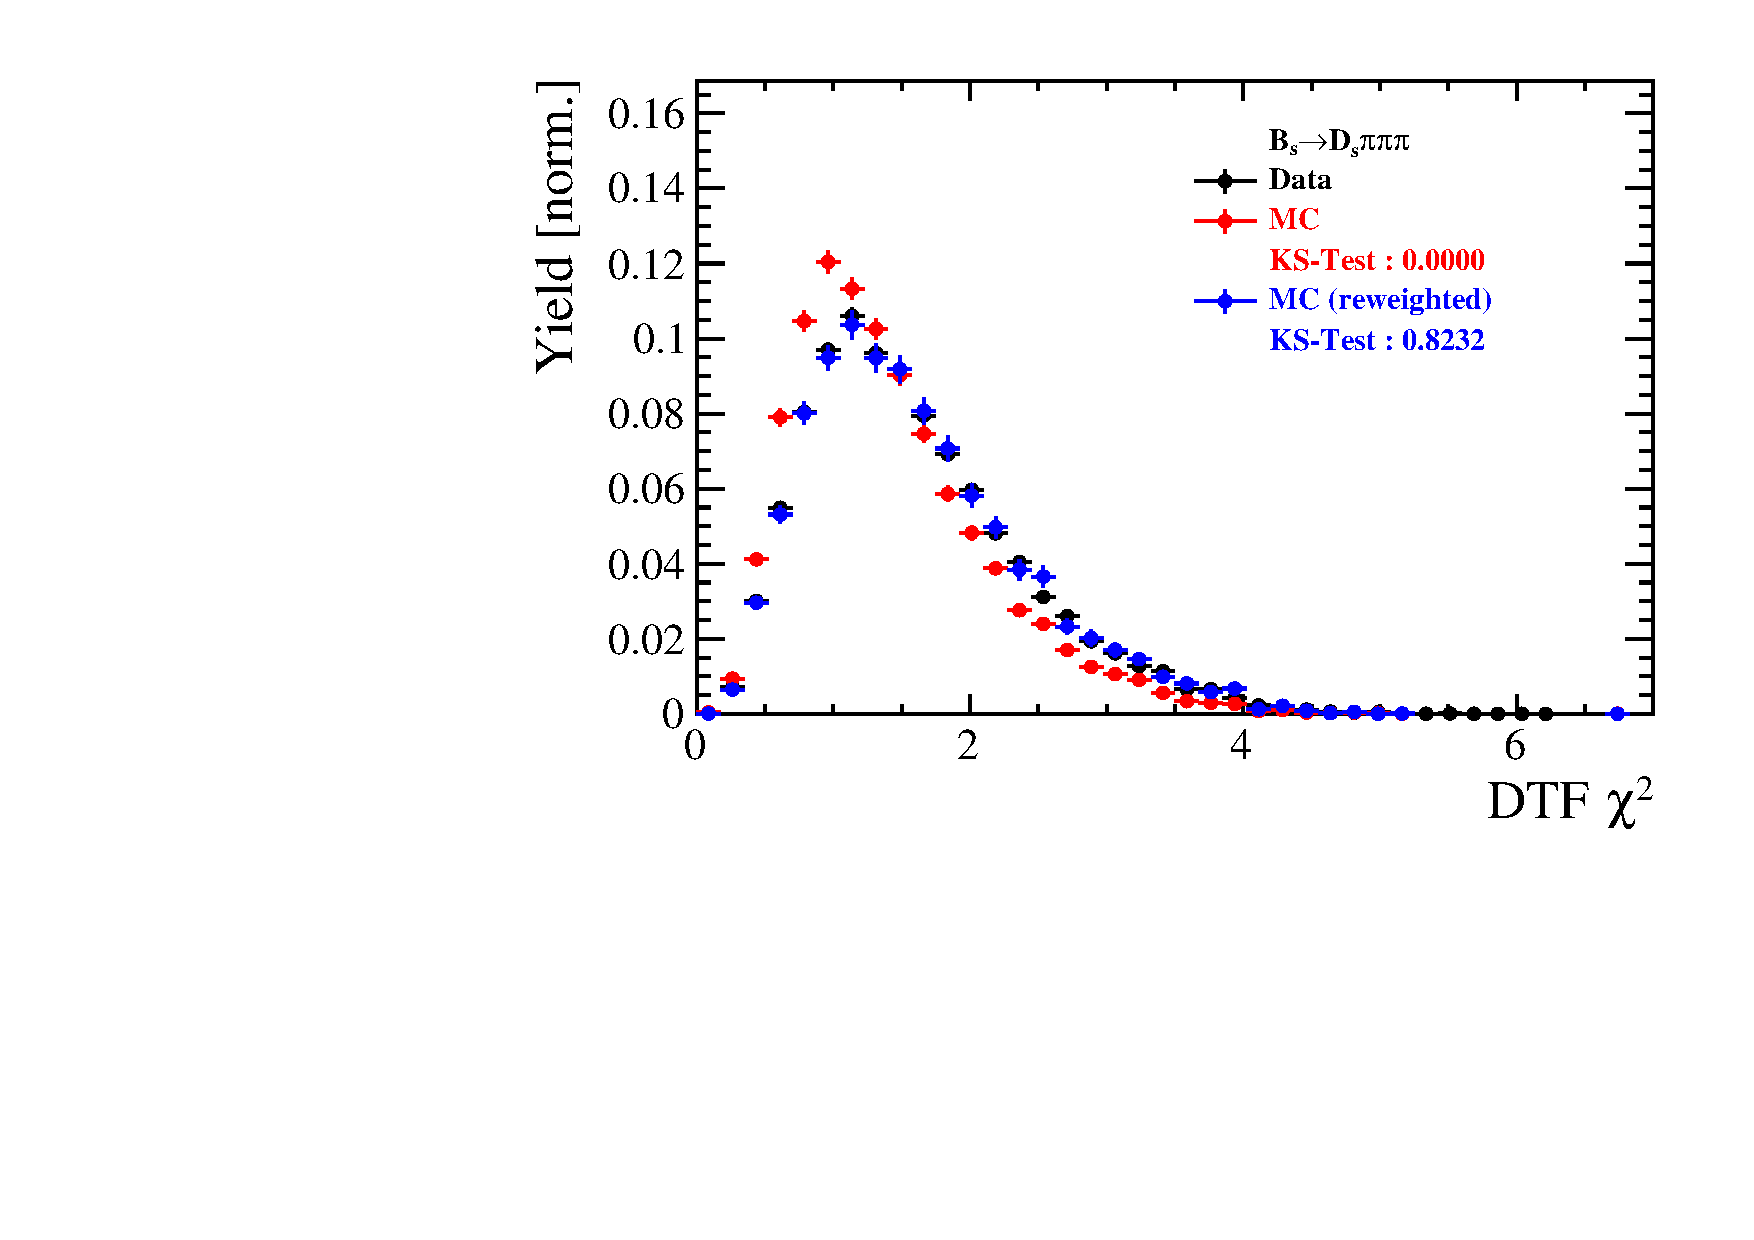
\includegraphics[height=!,width=0.4\textwidth]{figs/dataVsMC/norm_final/combined/Ds2KKpi_1_DTF_CHI2NDOF.pdf}
%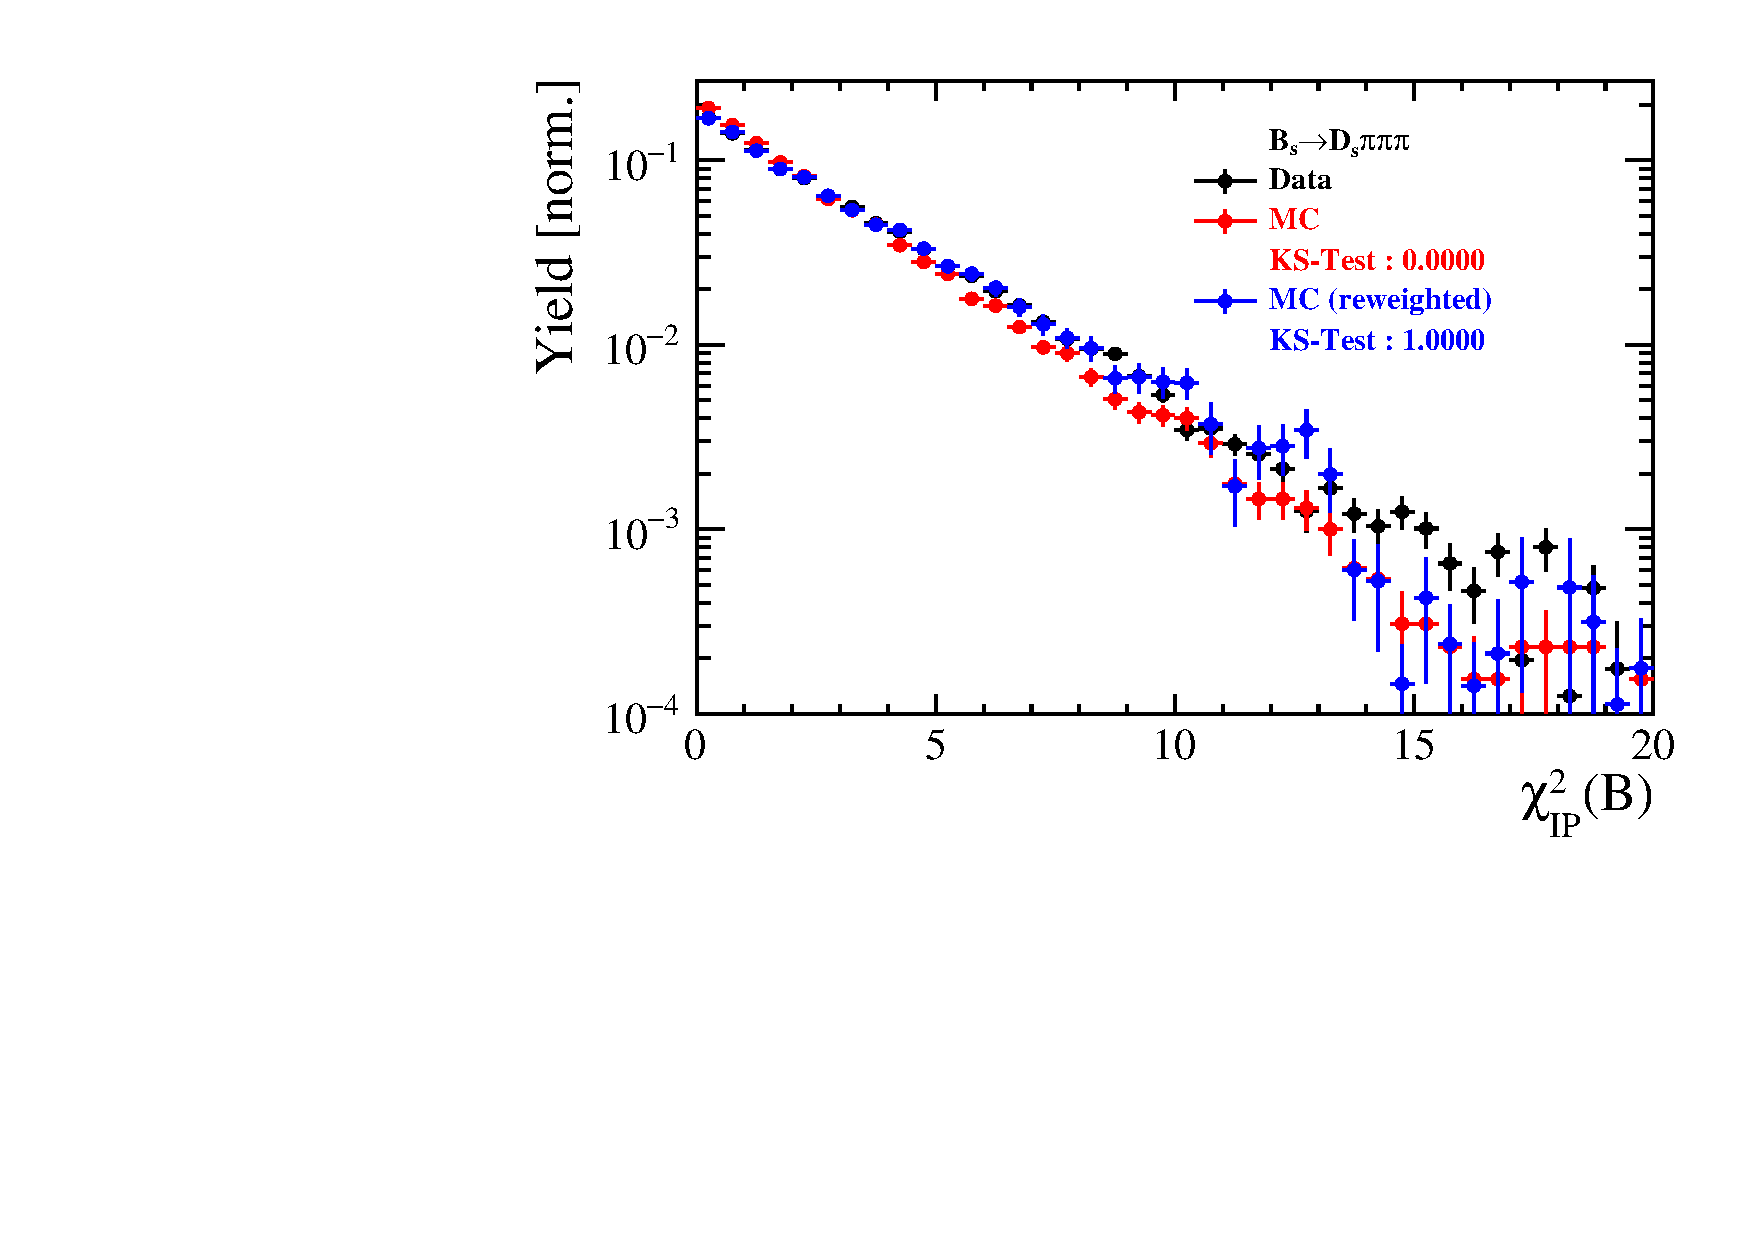
\includegraphics[height=!,width=0.4\textwidth]{figs/dataVsMC/norm_final/combined/Ds2KKpi_1_Bs_IPCHI2_OWNPV.pdf}
%
%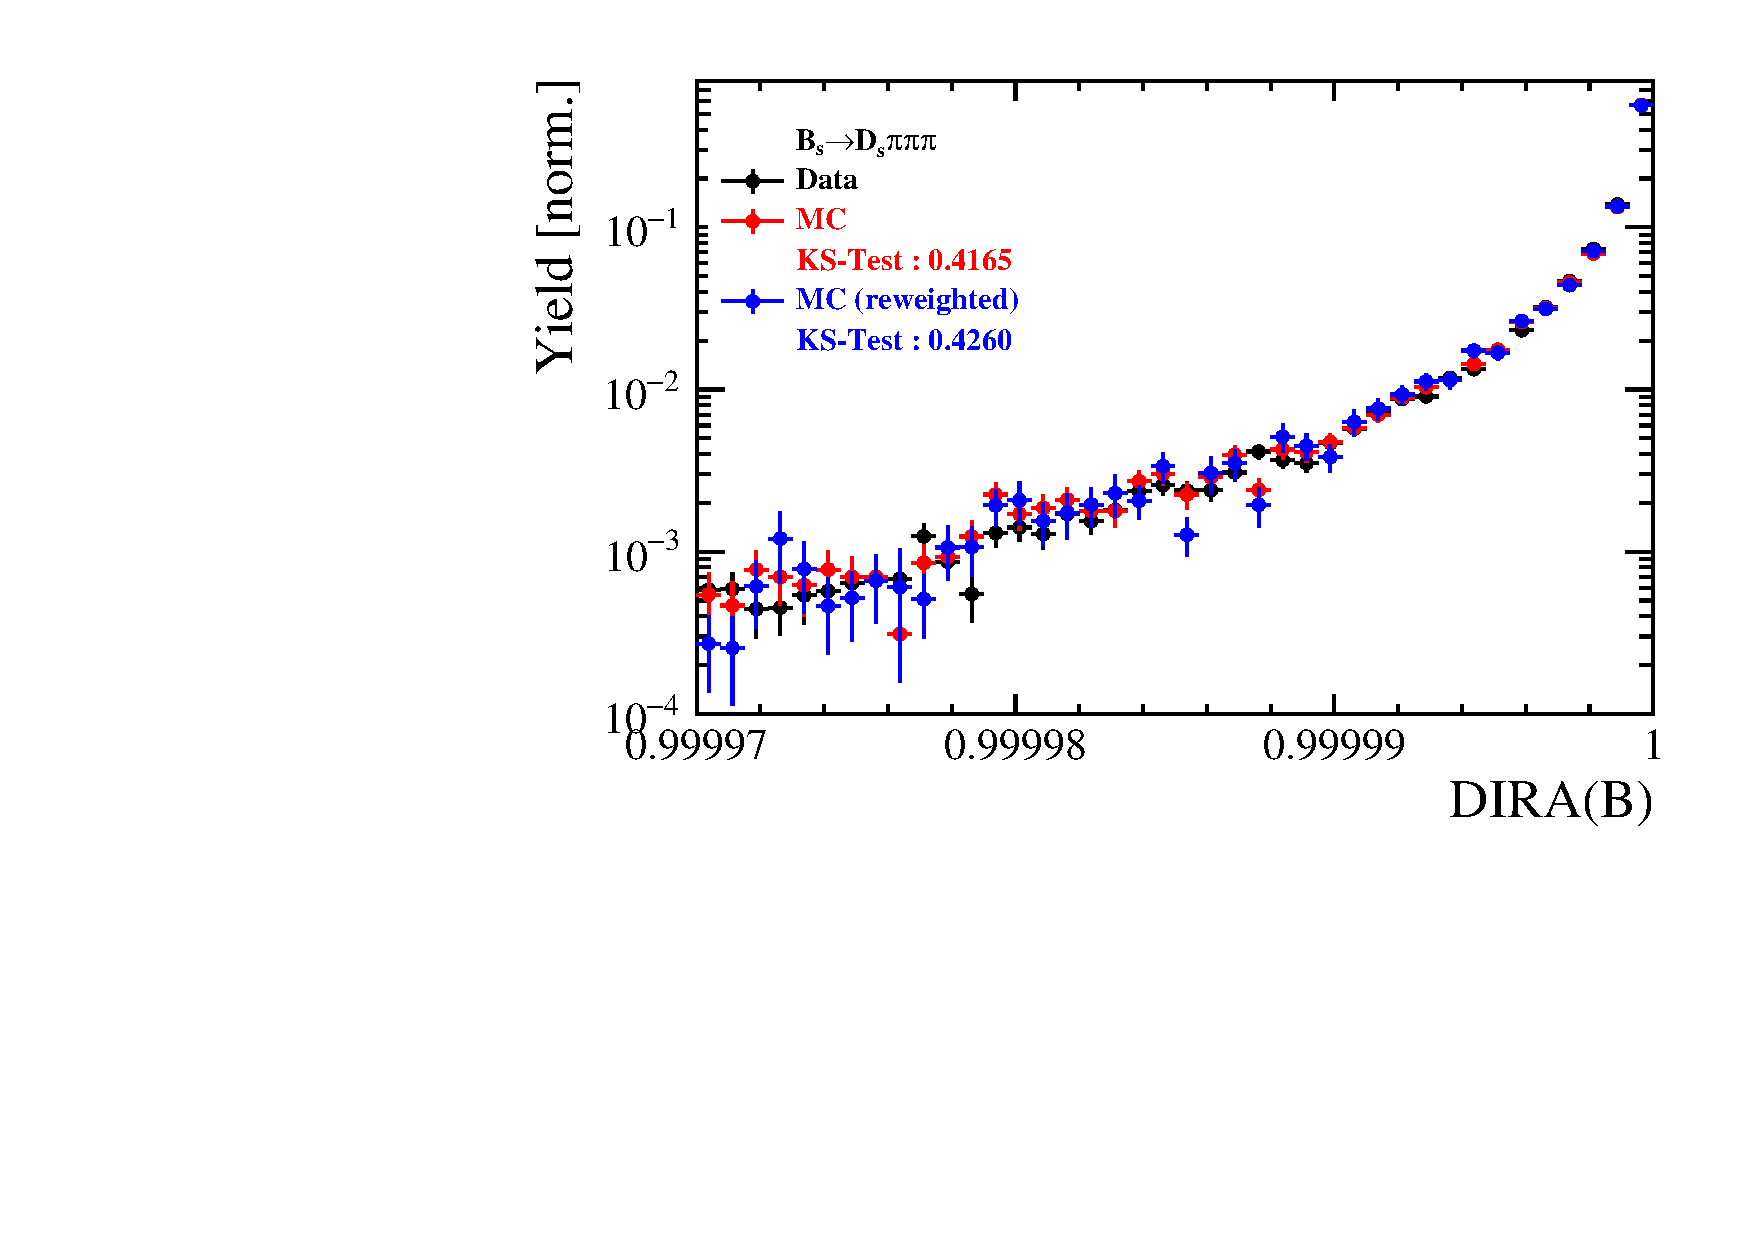
\includegraphics[height=!,width=0.4\textwidth]{figs/dataVsMC/norm_final/combined/Ds2KKpi_1_Bs_DIRA_OWNPV.pdf}
%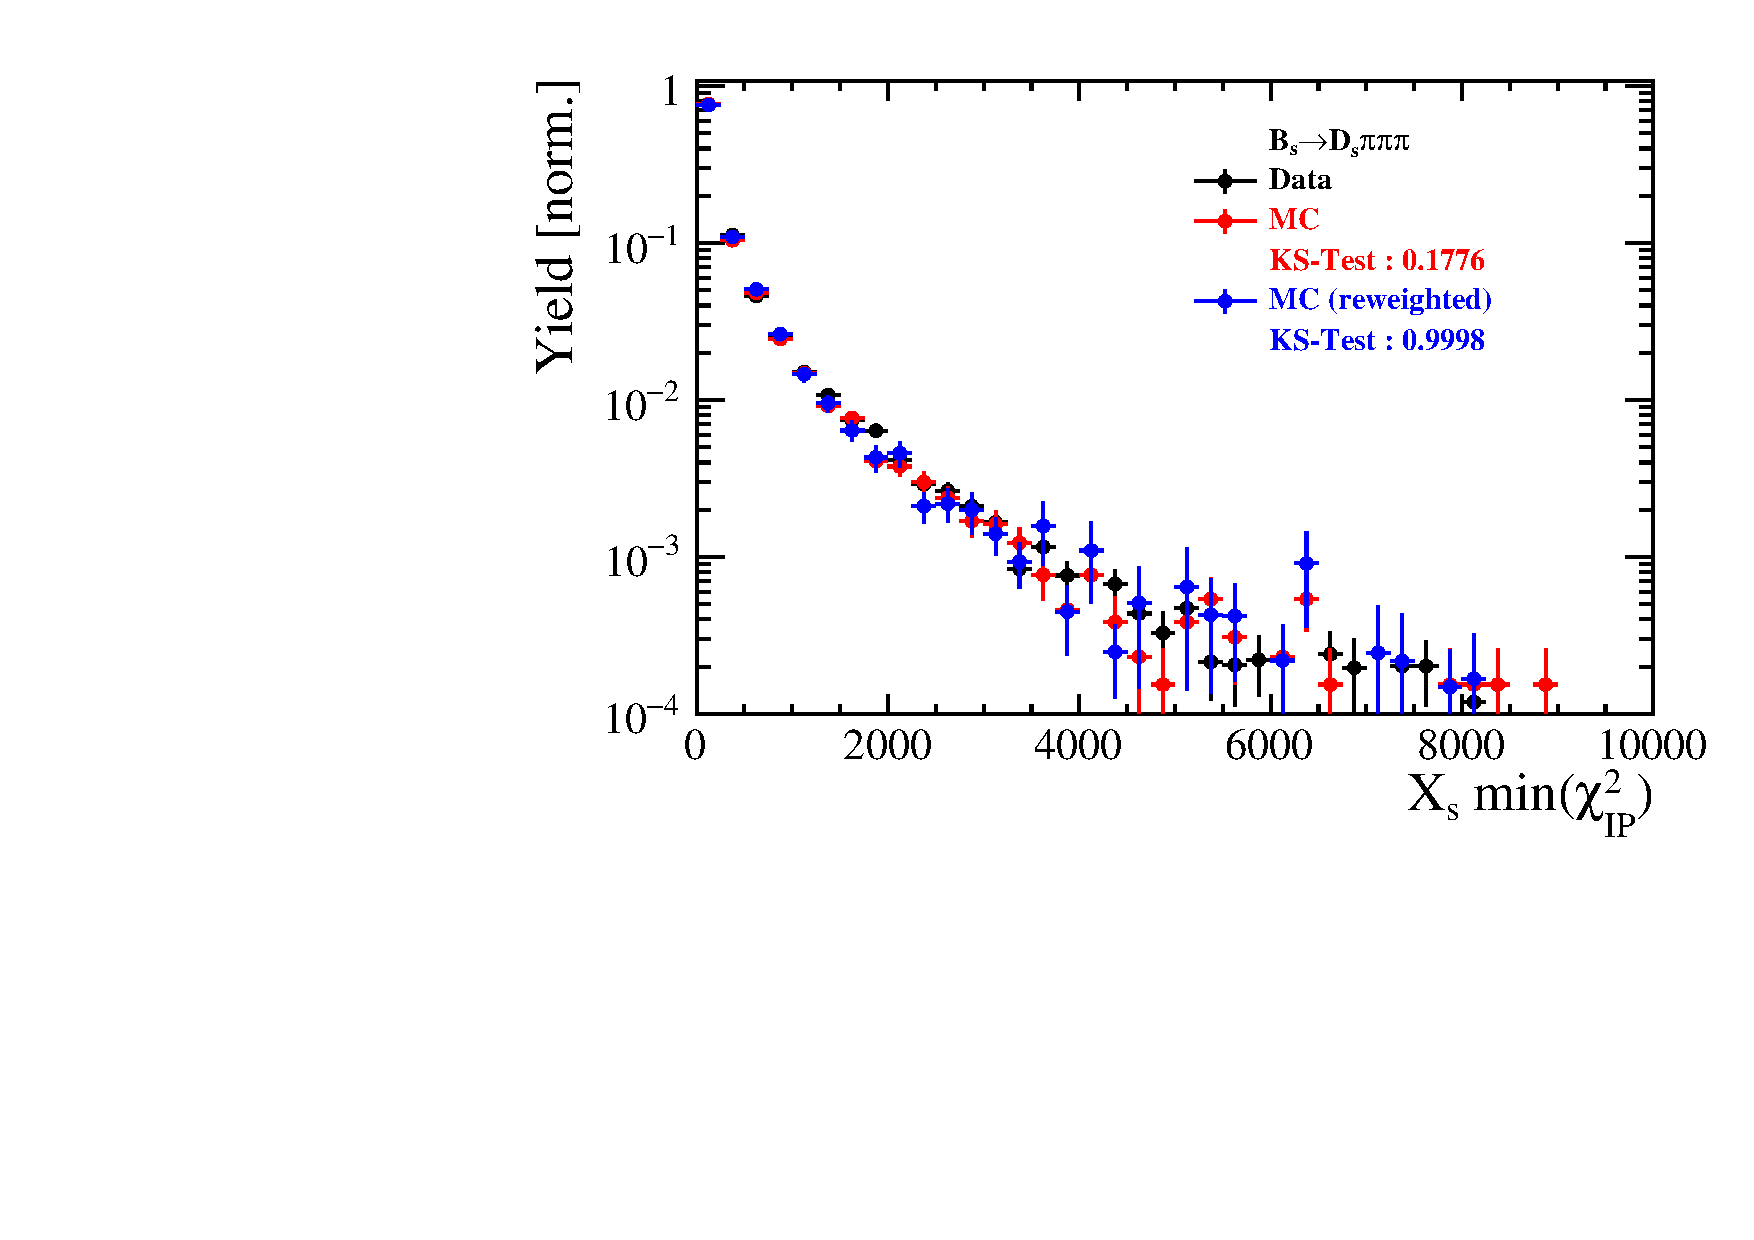
\includegraphics[height=!,width=0.4\textwidth]{figs/dataVsMC/norm_final/combined/Ds2KKpi_1_XsDaughters_min_IPCHI2.pdf}
%
%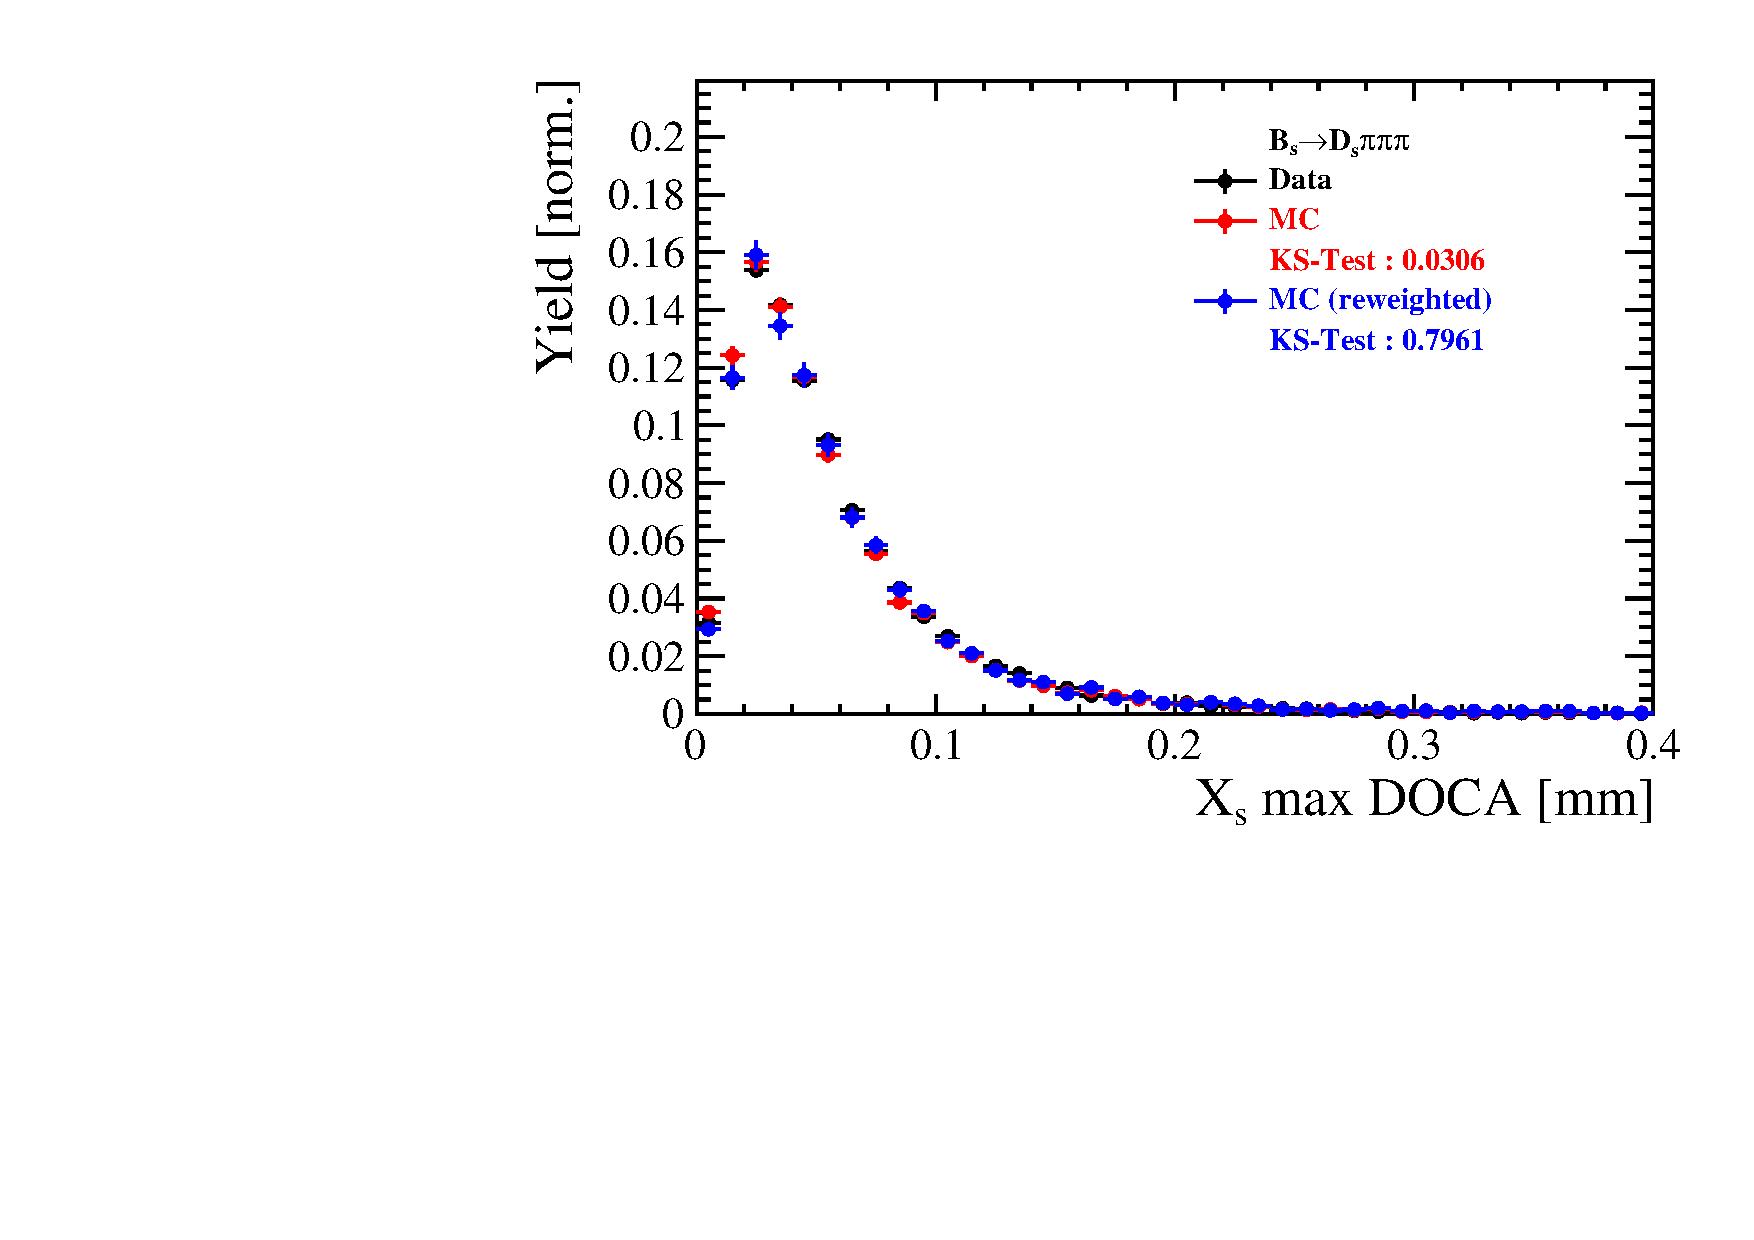
\includegraphics[height=!,width=0.4\textwidth]{figs/dataVsMC/norm_final/combined/Ds2KKpi_1_Xs_max_DOCA.pdf}
%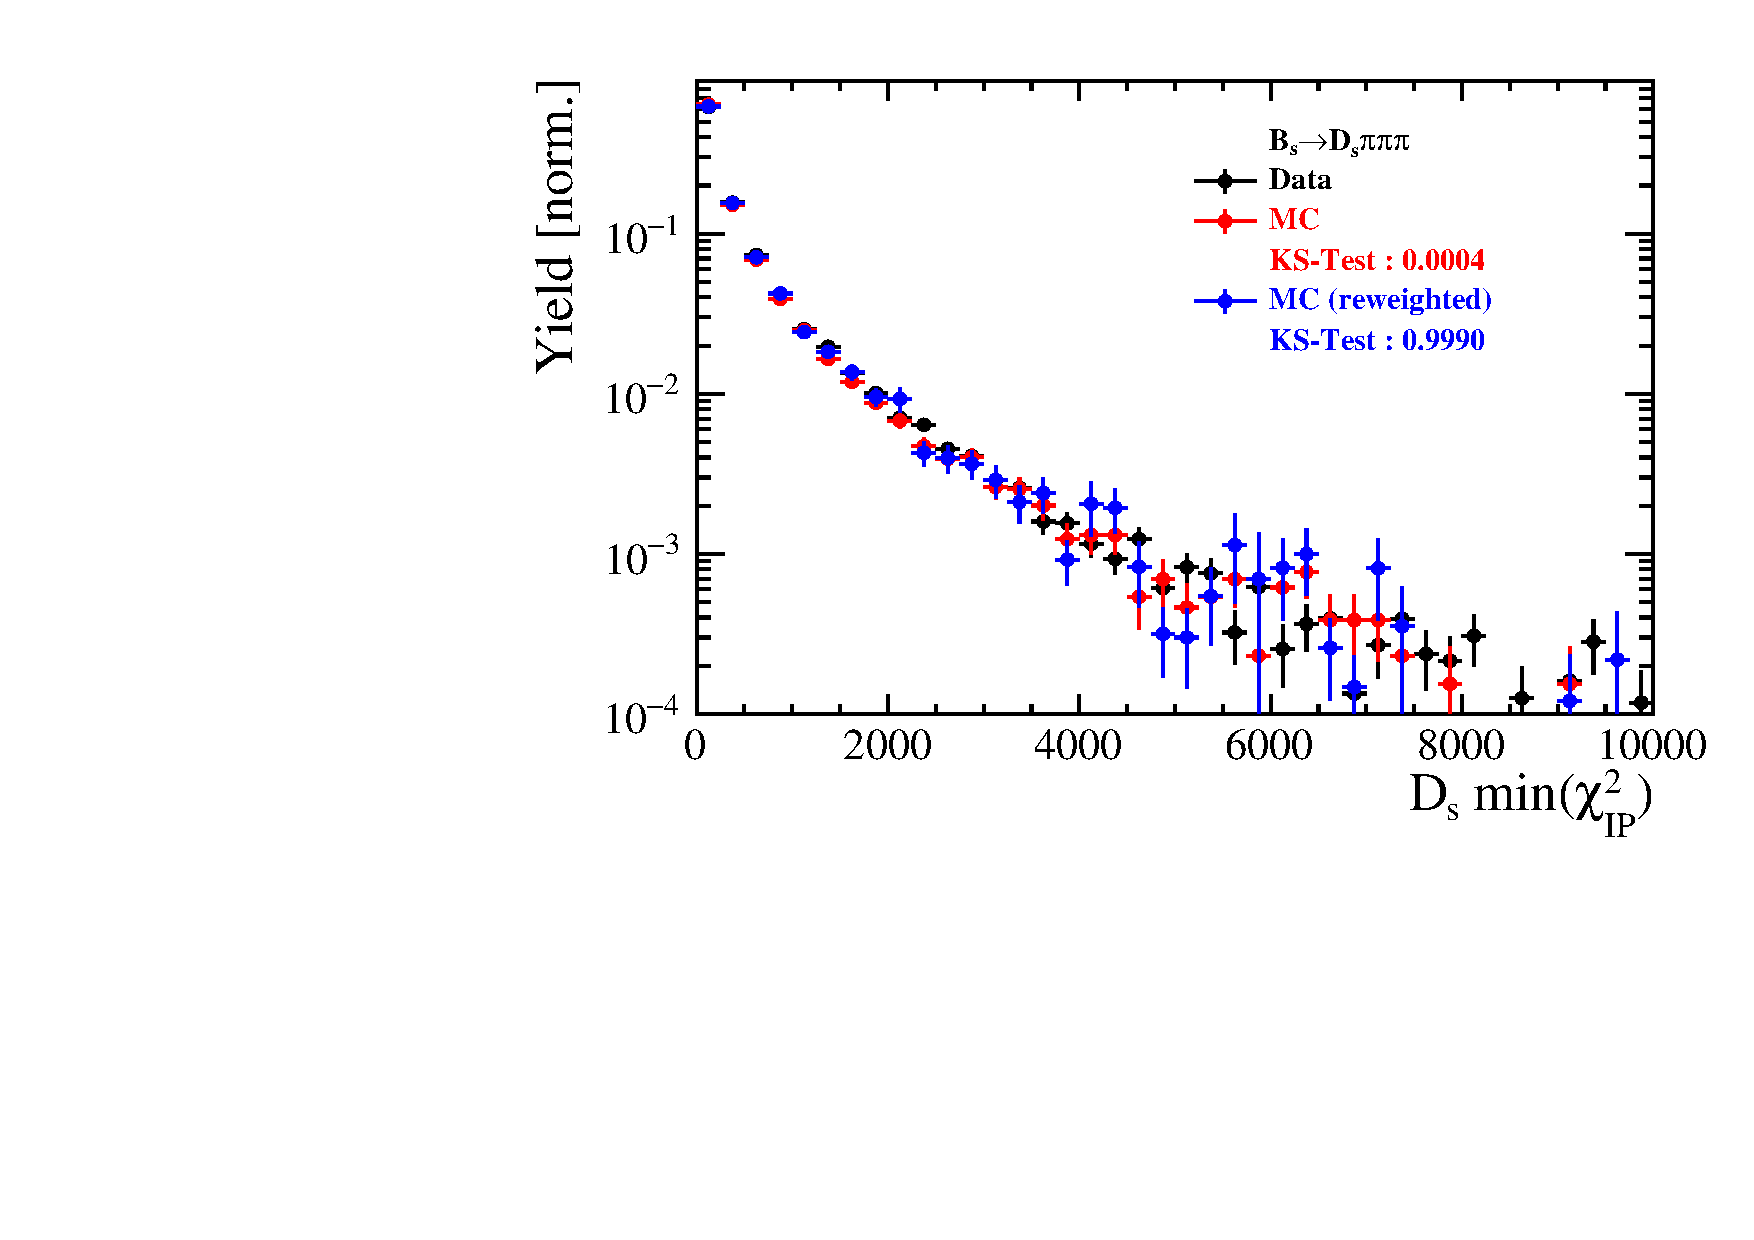
\includegraphics[height=!,width=0.4\textwidth]{figs/dataVsMC/norm_final/combined/Ds2KKpi_1_DsDaughters_min_IPCHI2.pdf}
%
%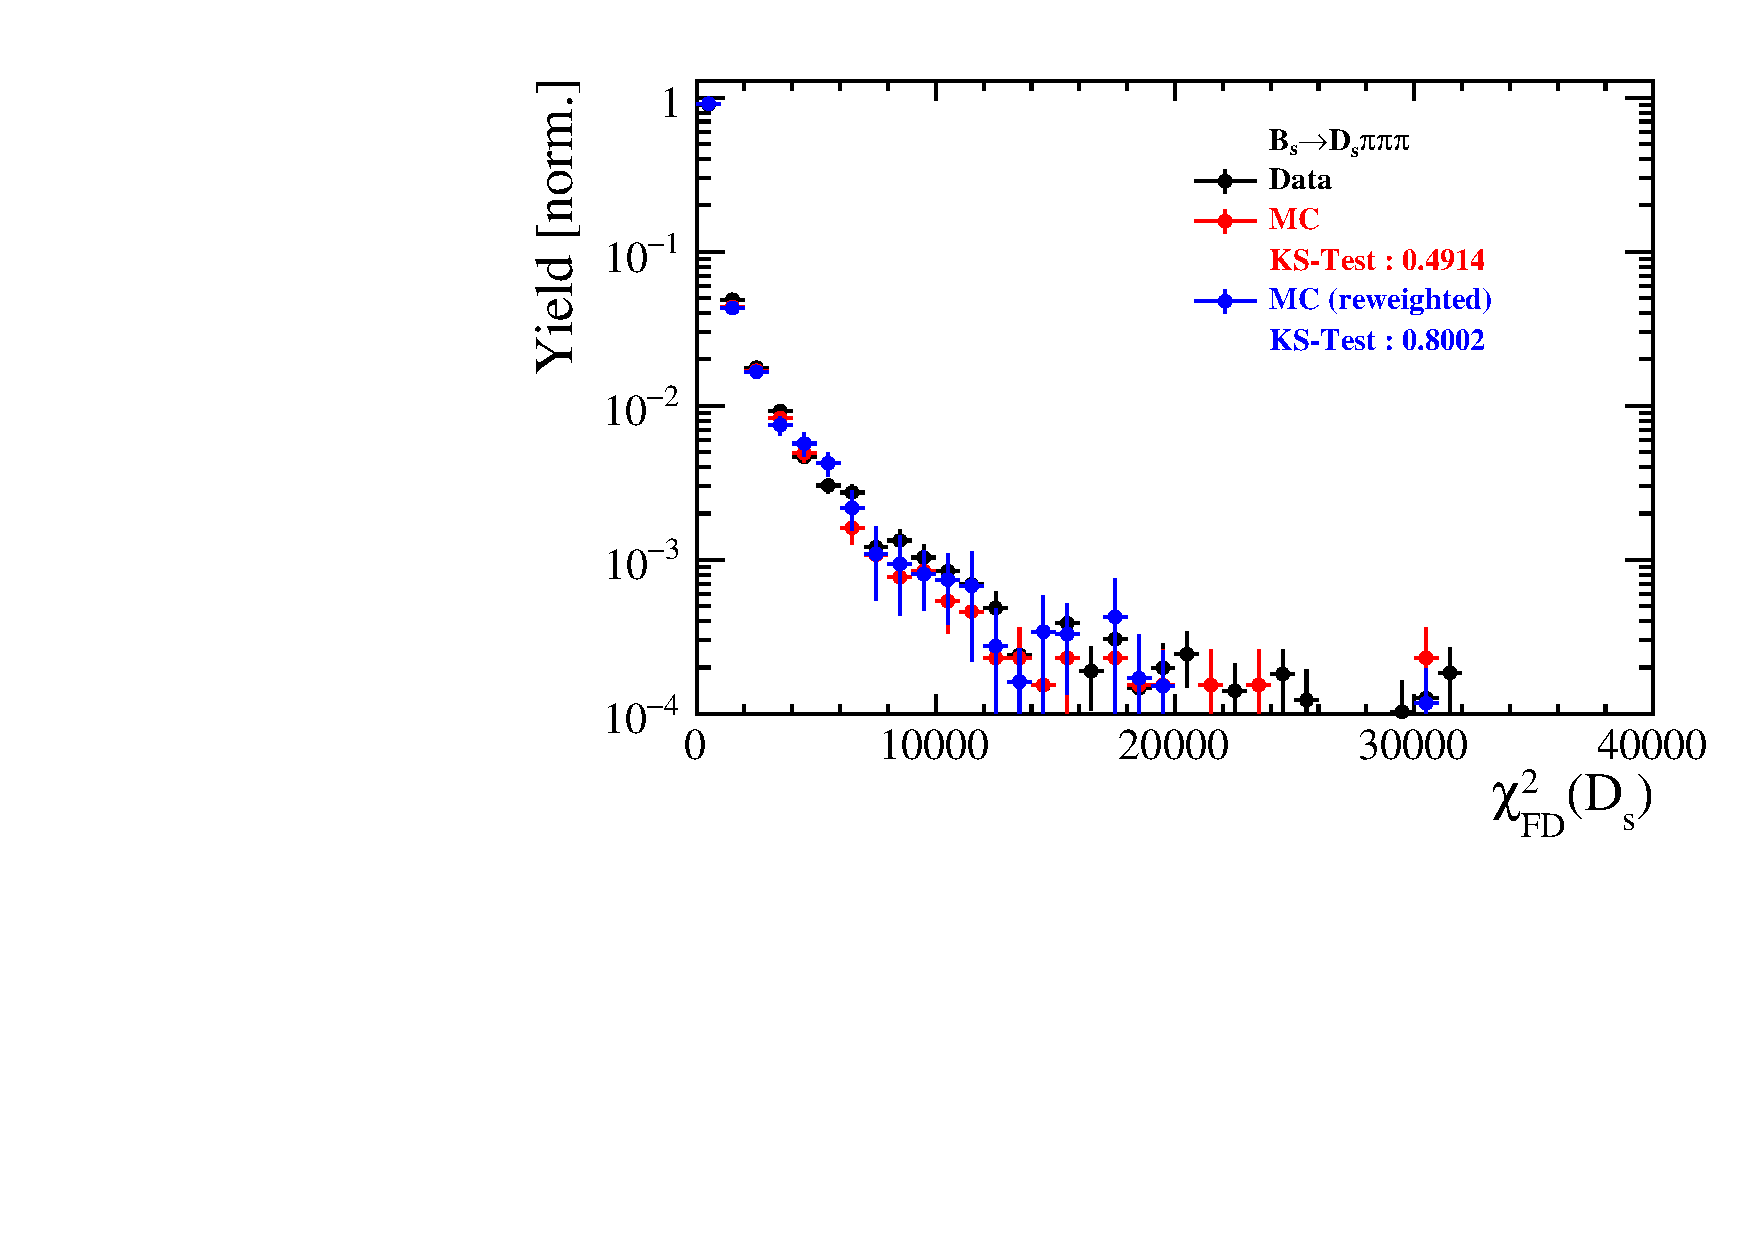
\includegraphics[height=!,width=0.4\textwidth]{figs/dataVsMC/norm_final/combined/Ds2KKpi_1_Ds_FDCHI2_ORIVX.pdf}
%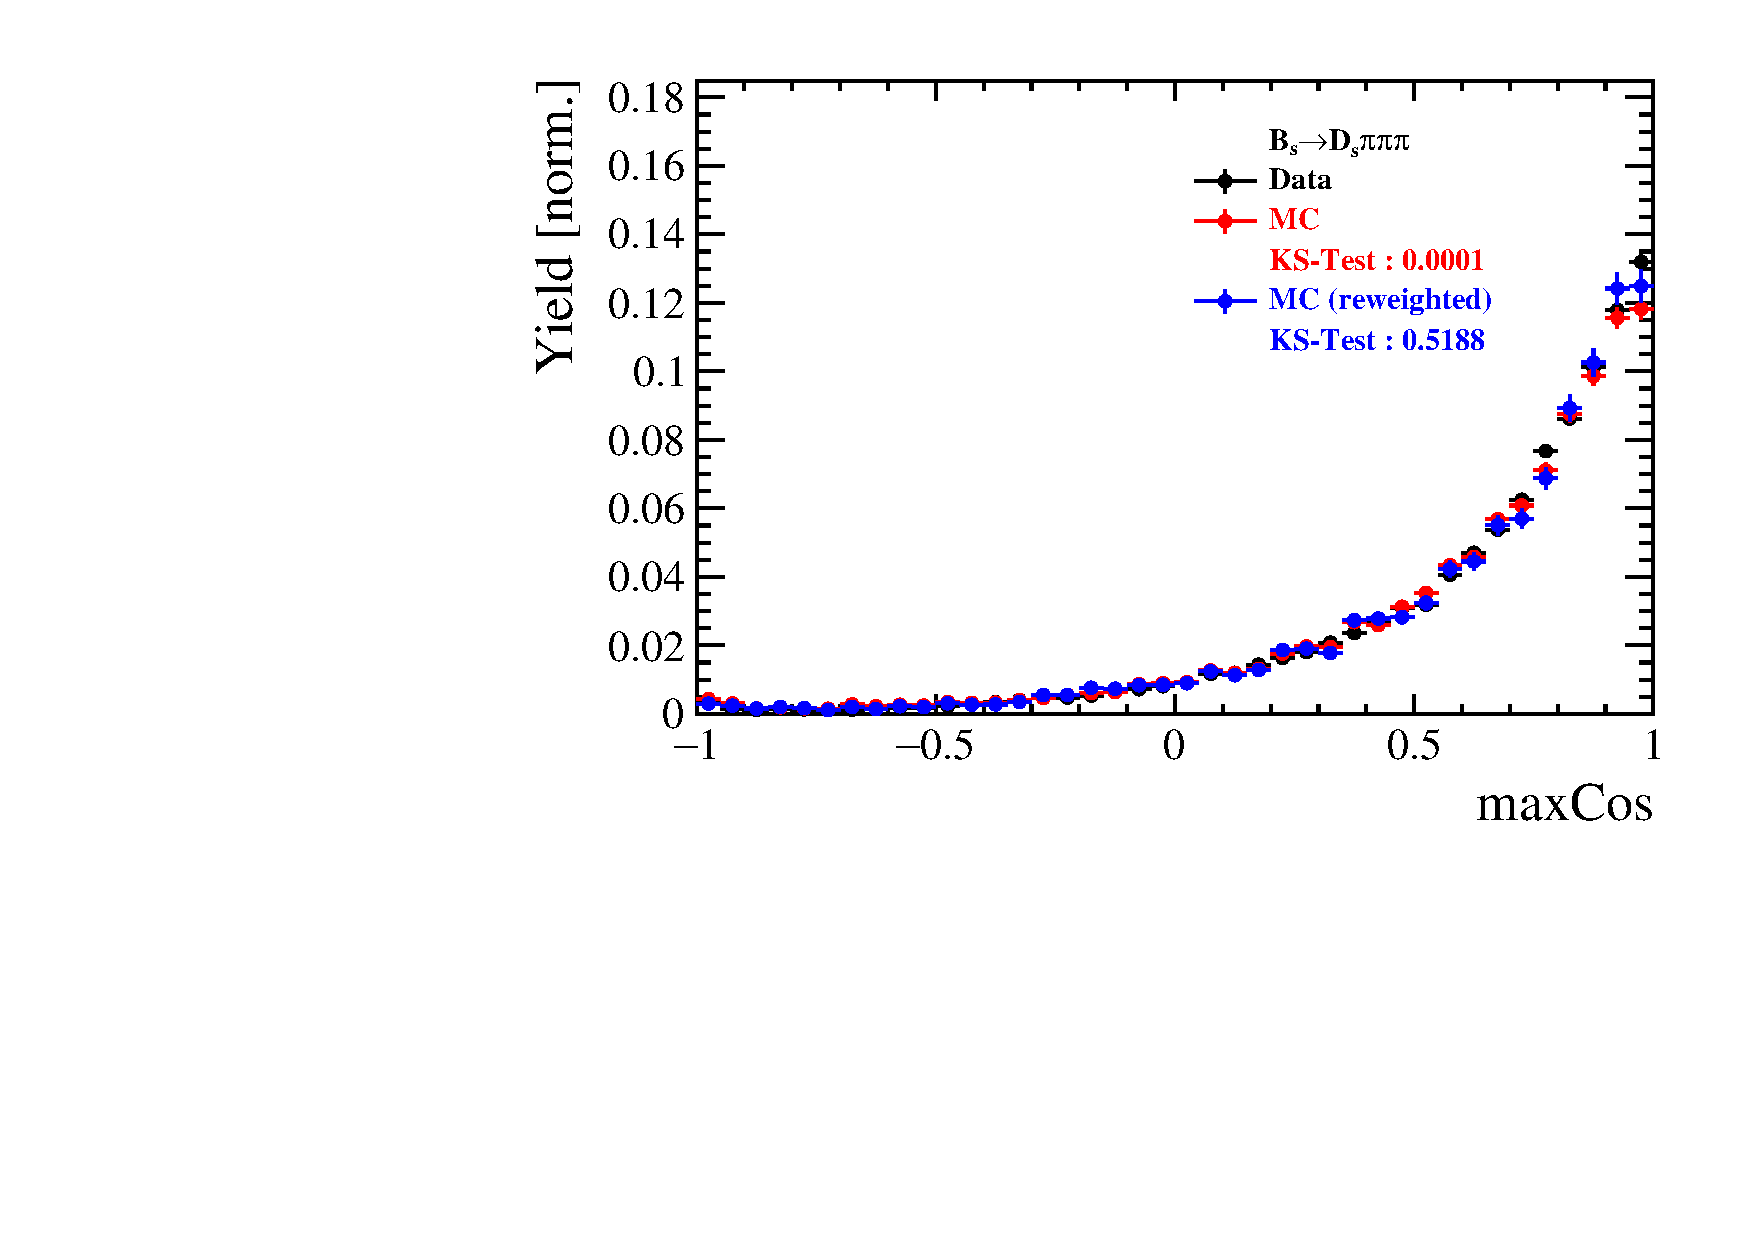
\includegraphics[height=!,width=0.4\textwidth]{figs/dataVsMC/norm_final/combined/Ds2KKpi_1_maxCos.pdf}
%
%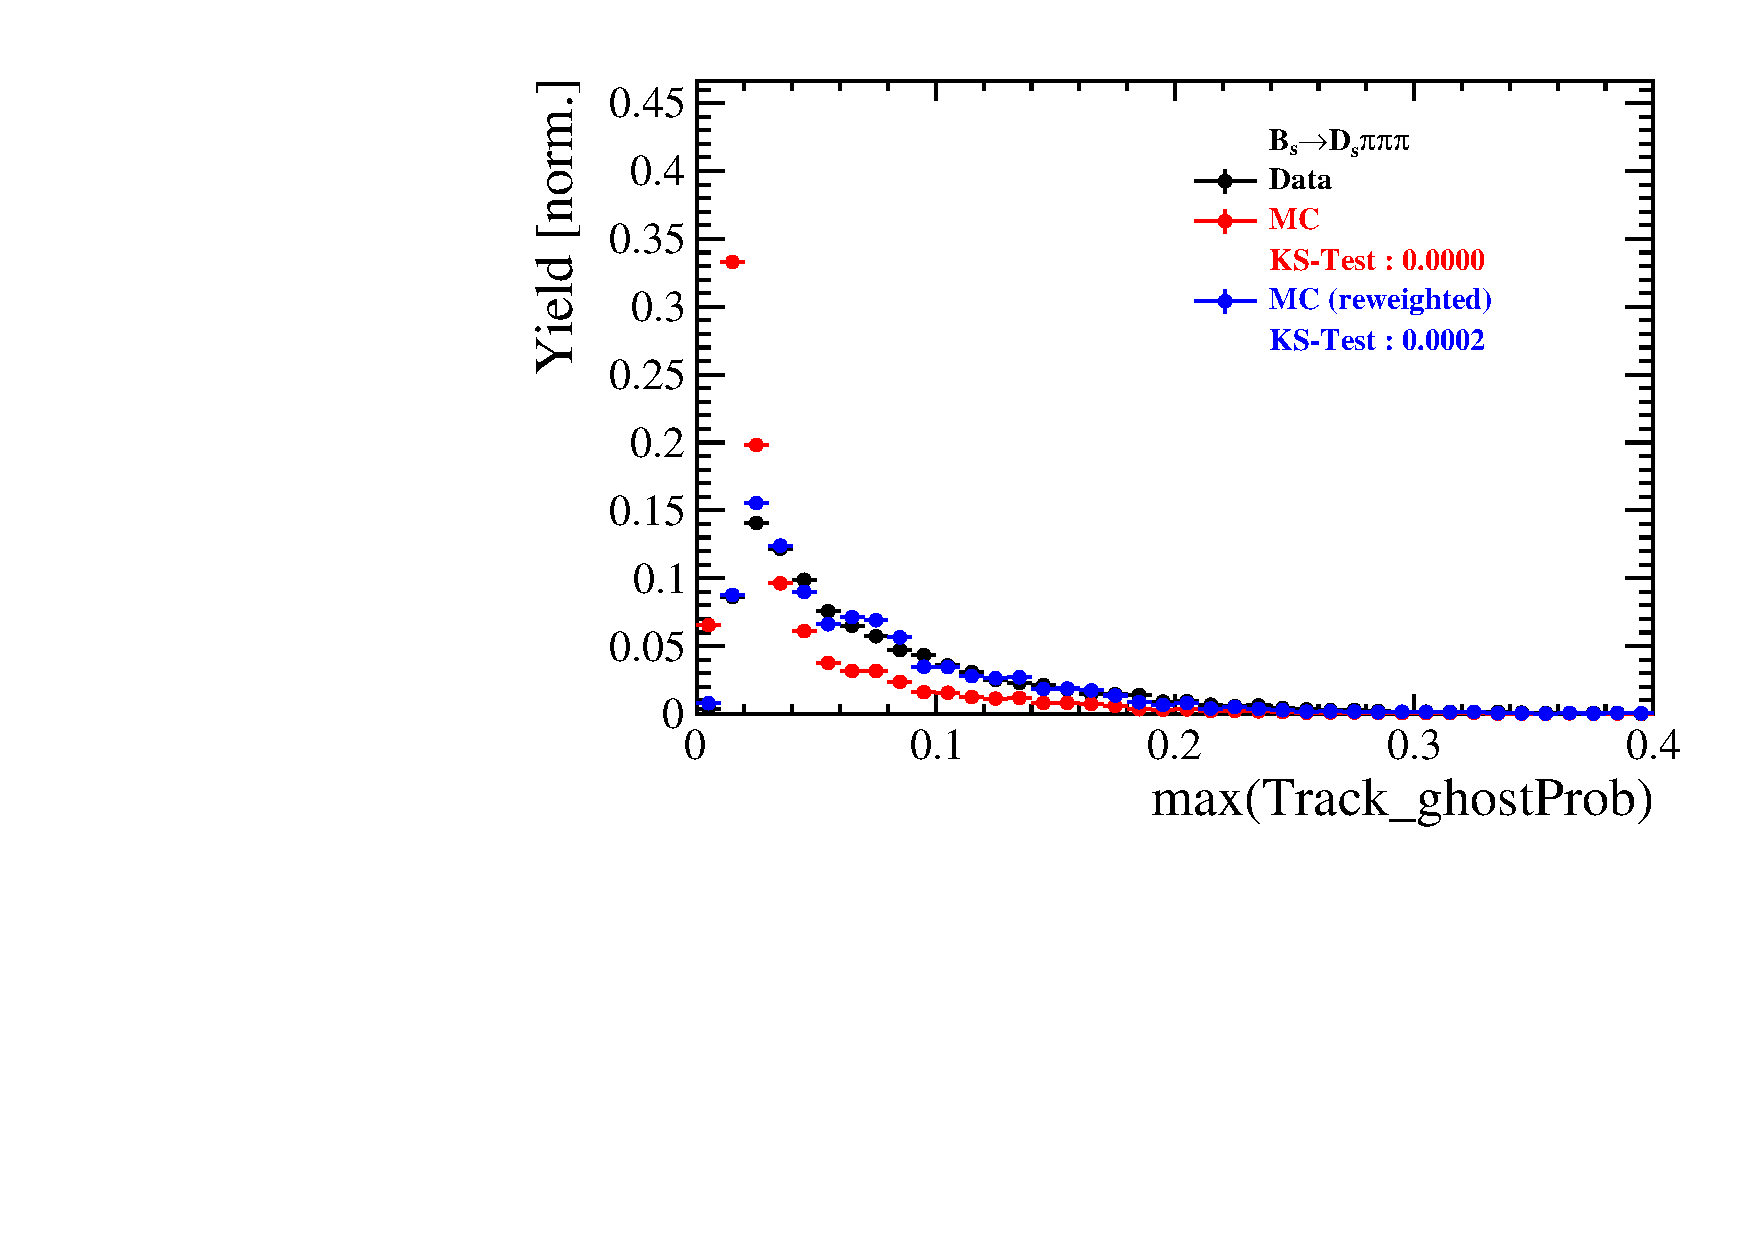
\includegraphics[height=!,width=0.4\textwidth]{figs/dataVsMC/norm_final/combined/Ds2KKpi_1_max_ghostProb.pdf}
%%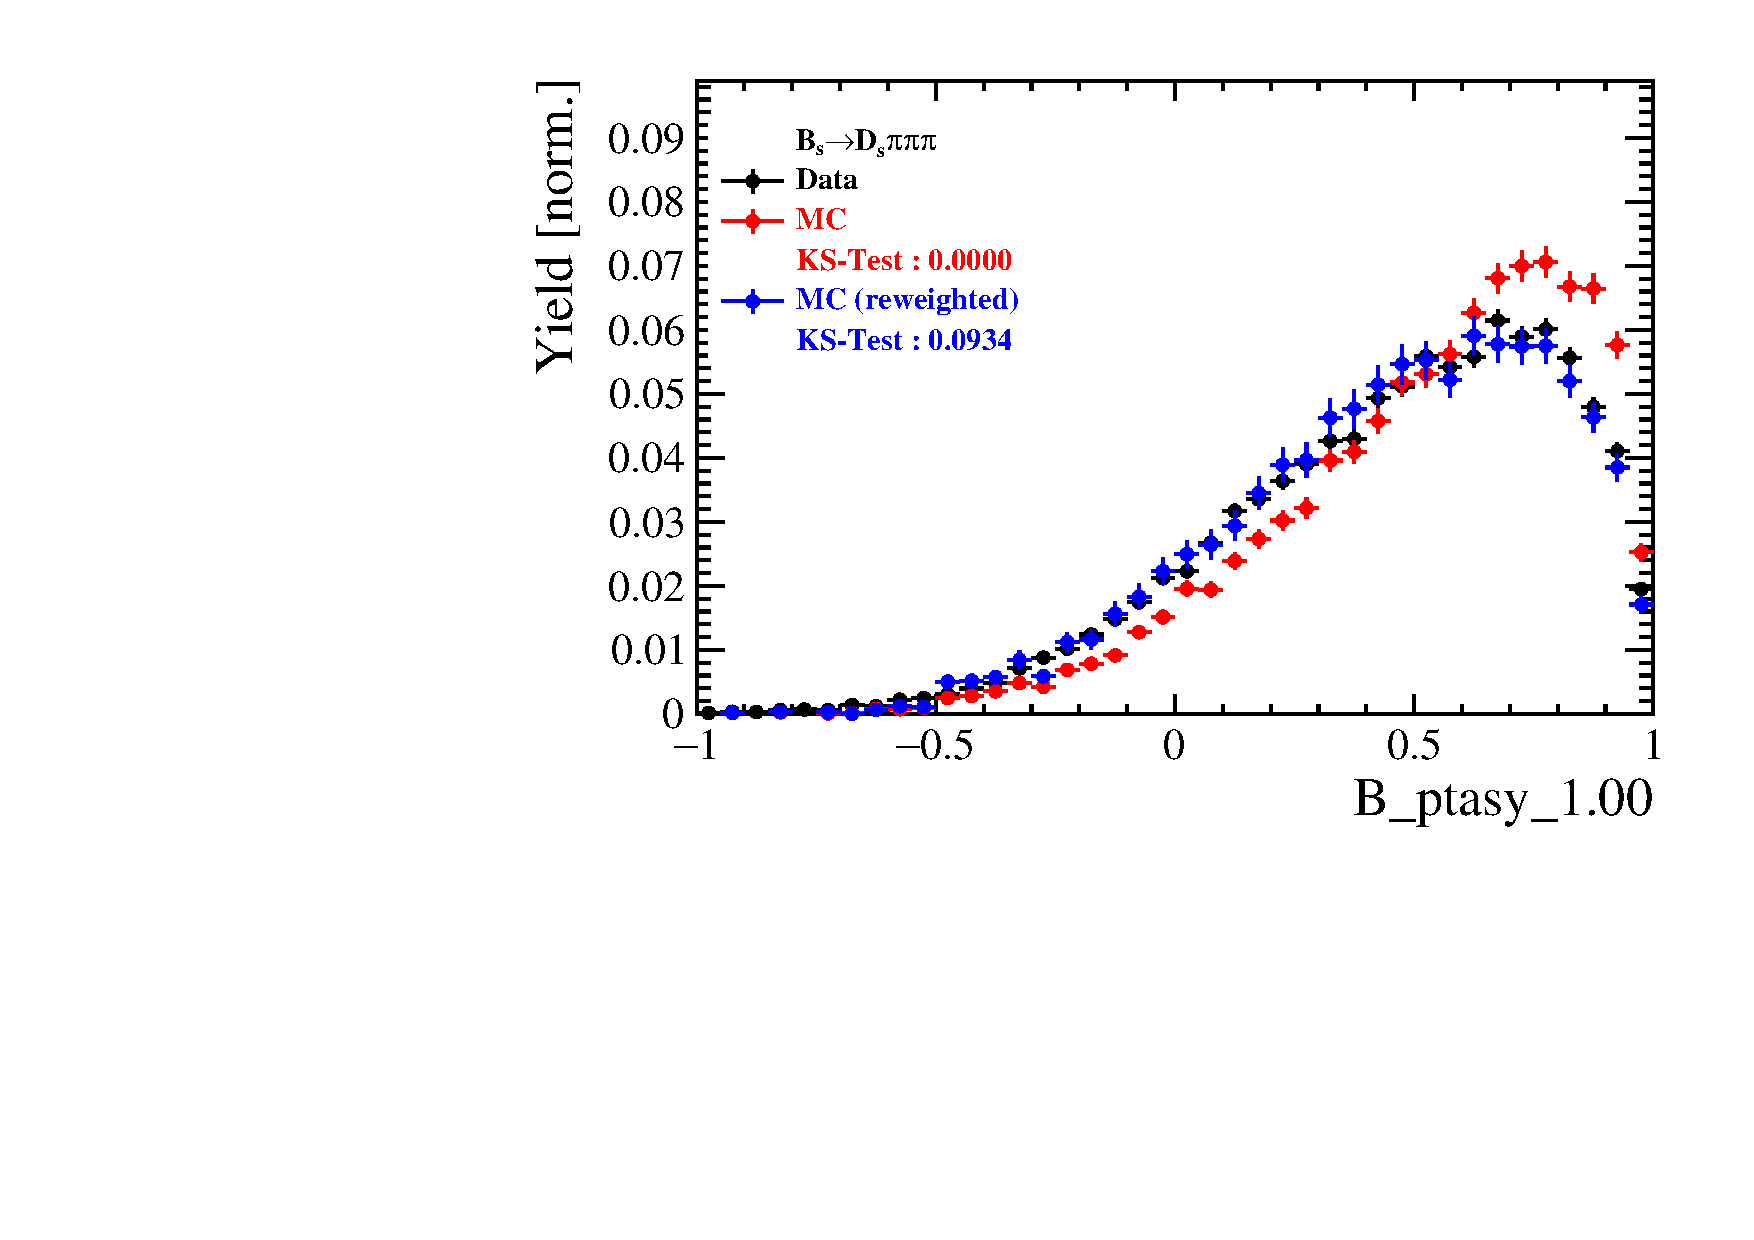
\includegraphics[height=!,width=0.5\textwidth]{figs/dataVsMC/norm_final/combined/Ds2KKpi_1_Bs_ptasy_1.00.pdf}
%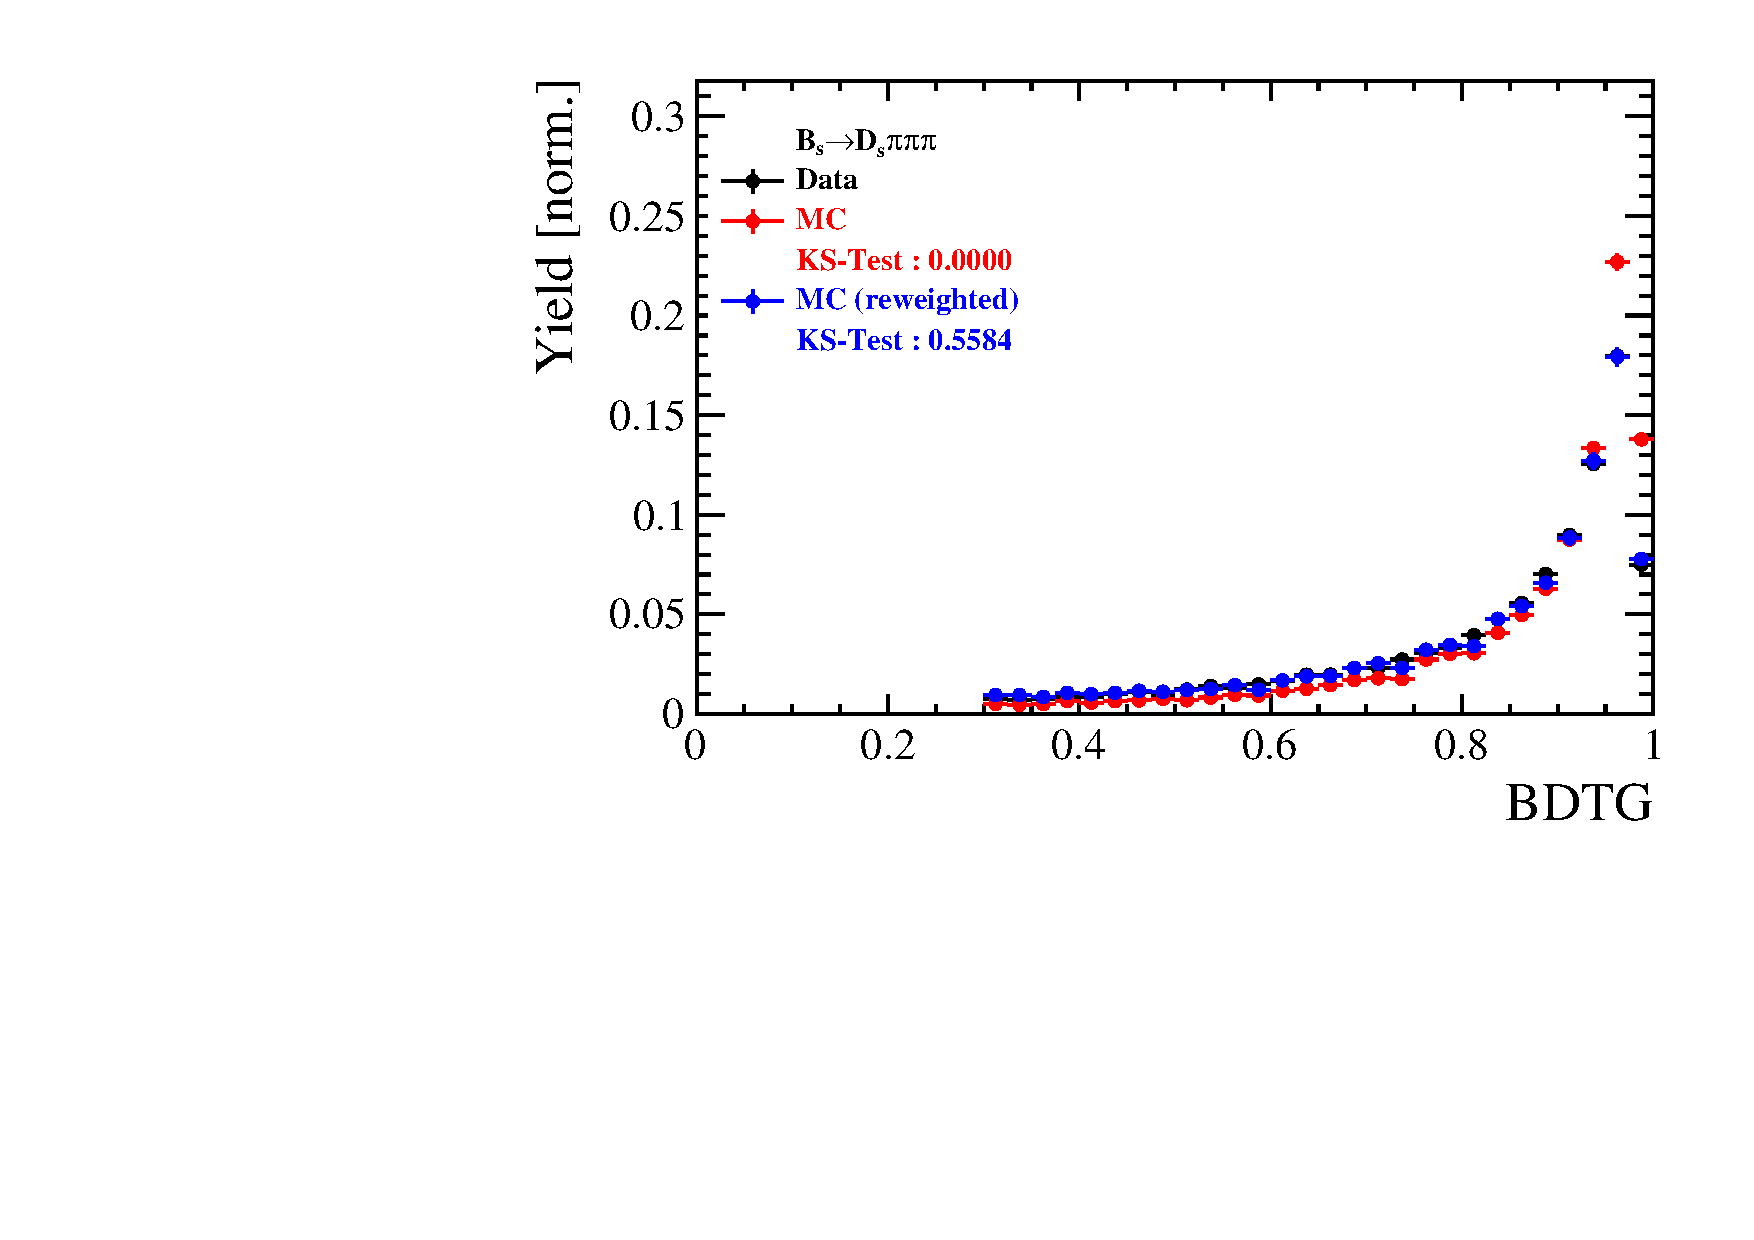
\includegraphics[height=!,width=0.4\textwidth]{figs/dataVsMC/norm_final/combined/Ds2KKpi_1_BDTG_response.pdf}
%
%\caption{Comparison of BDTG input variables and classifier response for $B_s\to D_s\pi\pi\pi$ decays.}
%\label{fig:}
%\end{figure}



%\begin{figure}[h]
\centering
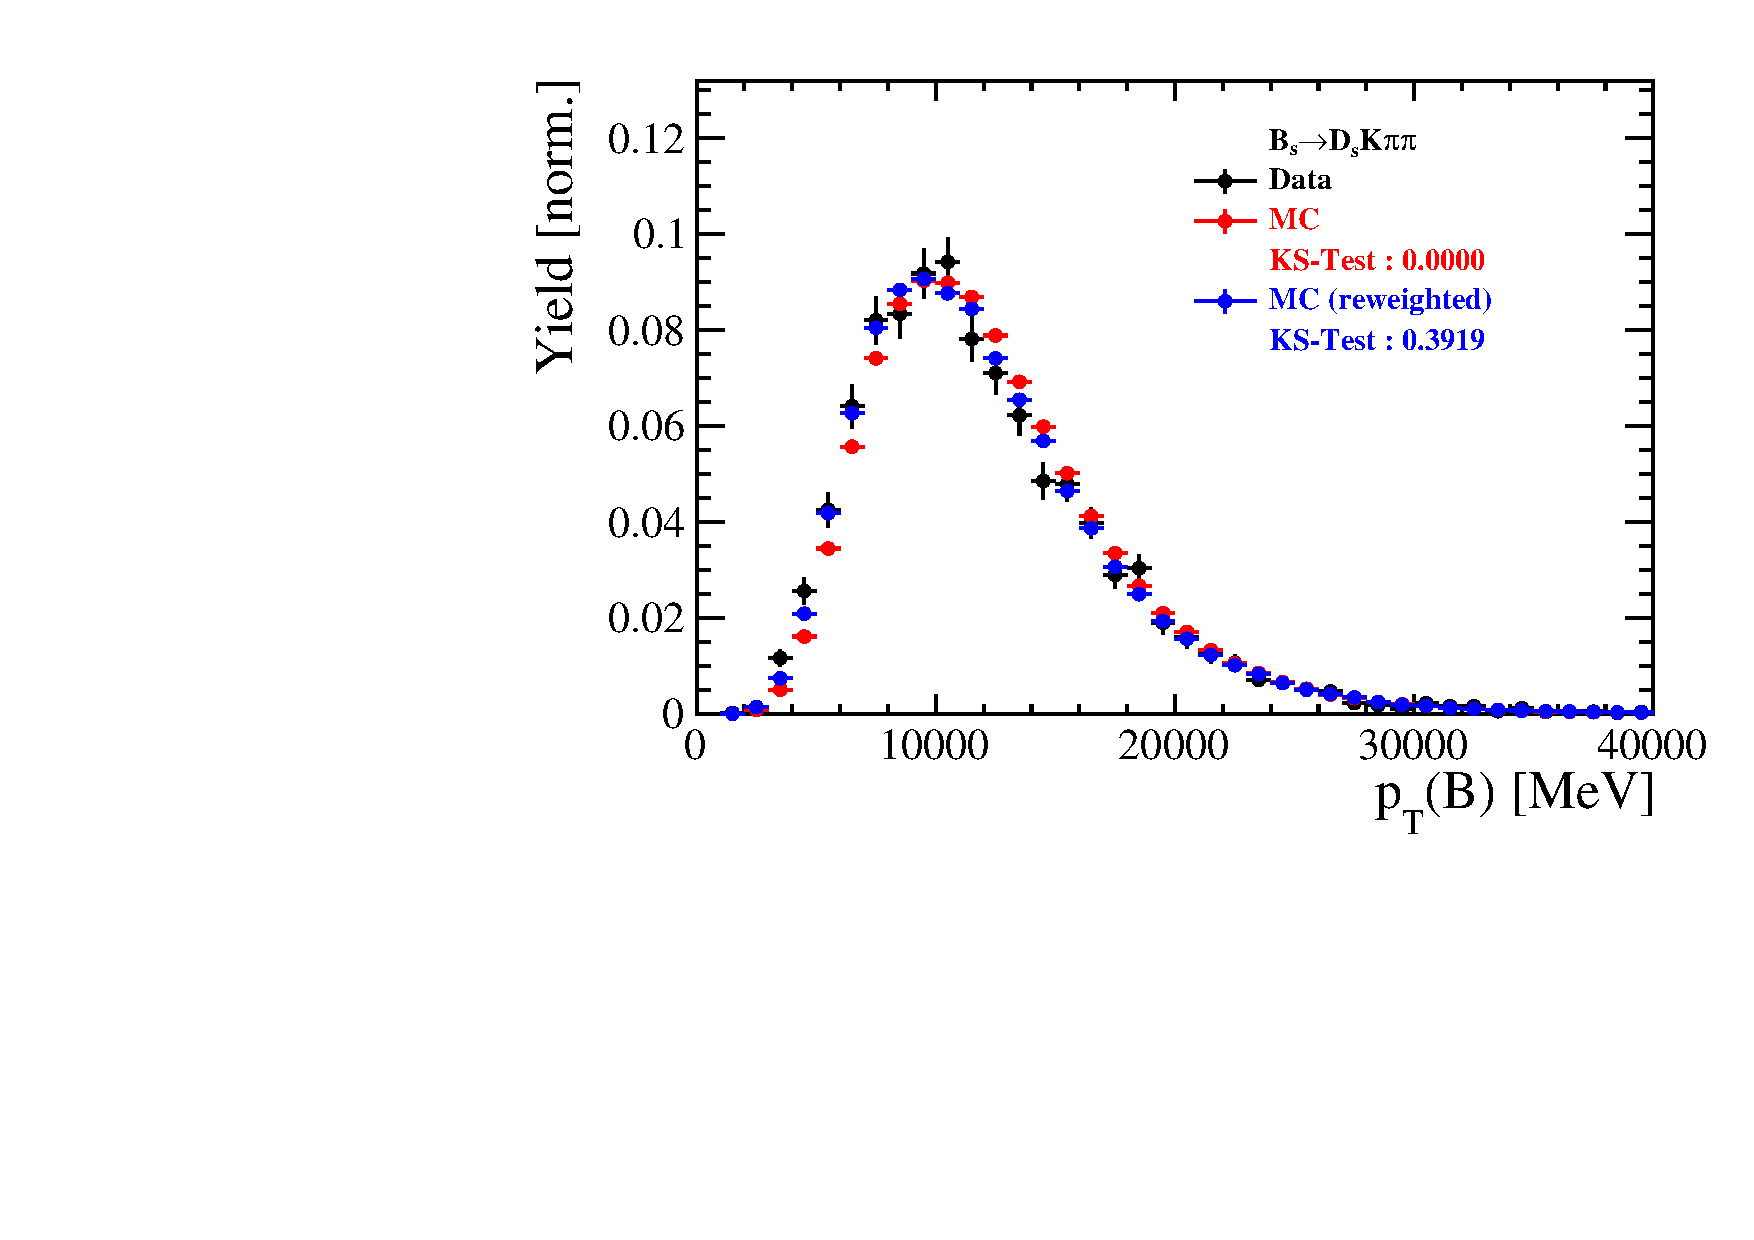
\includegraphics[height=!,width=0.3\textwidth]{figs/dataVsMC/signal_final/combined/Ds2all_Bs_PT.pdf}
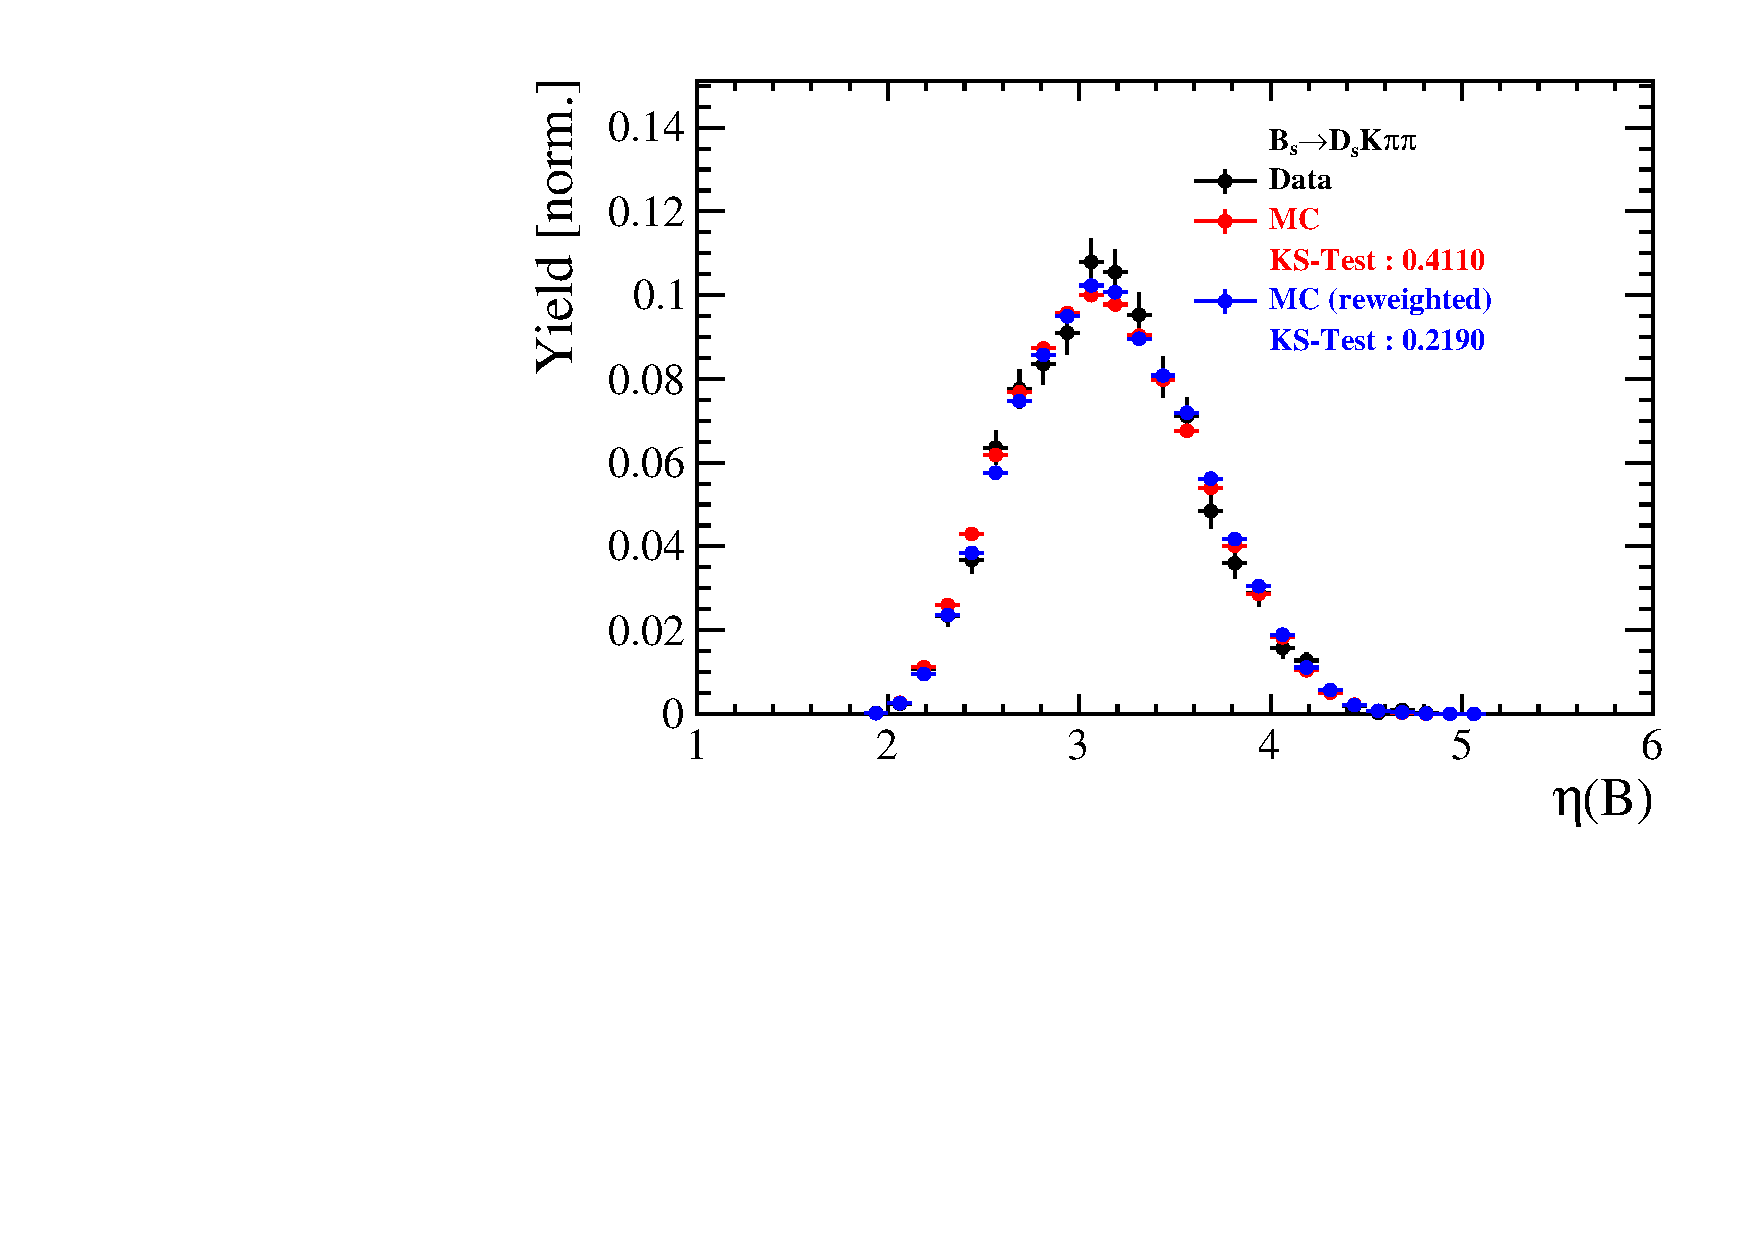
\includegraphics[height=!,width=0.3\textwidth]{figs/dataVsMC/signal_final/combined/Ds2all_Bs_ETA.pdf}
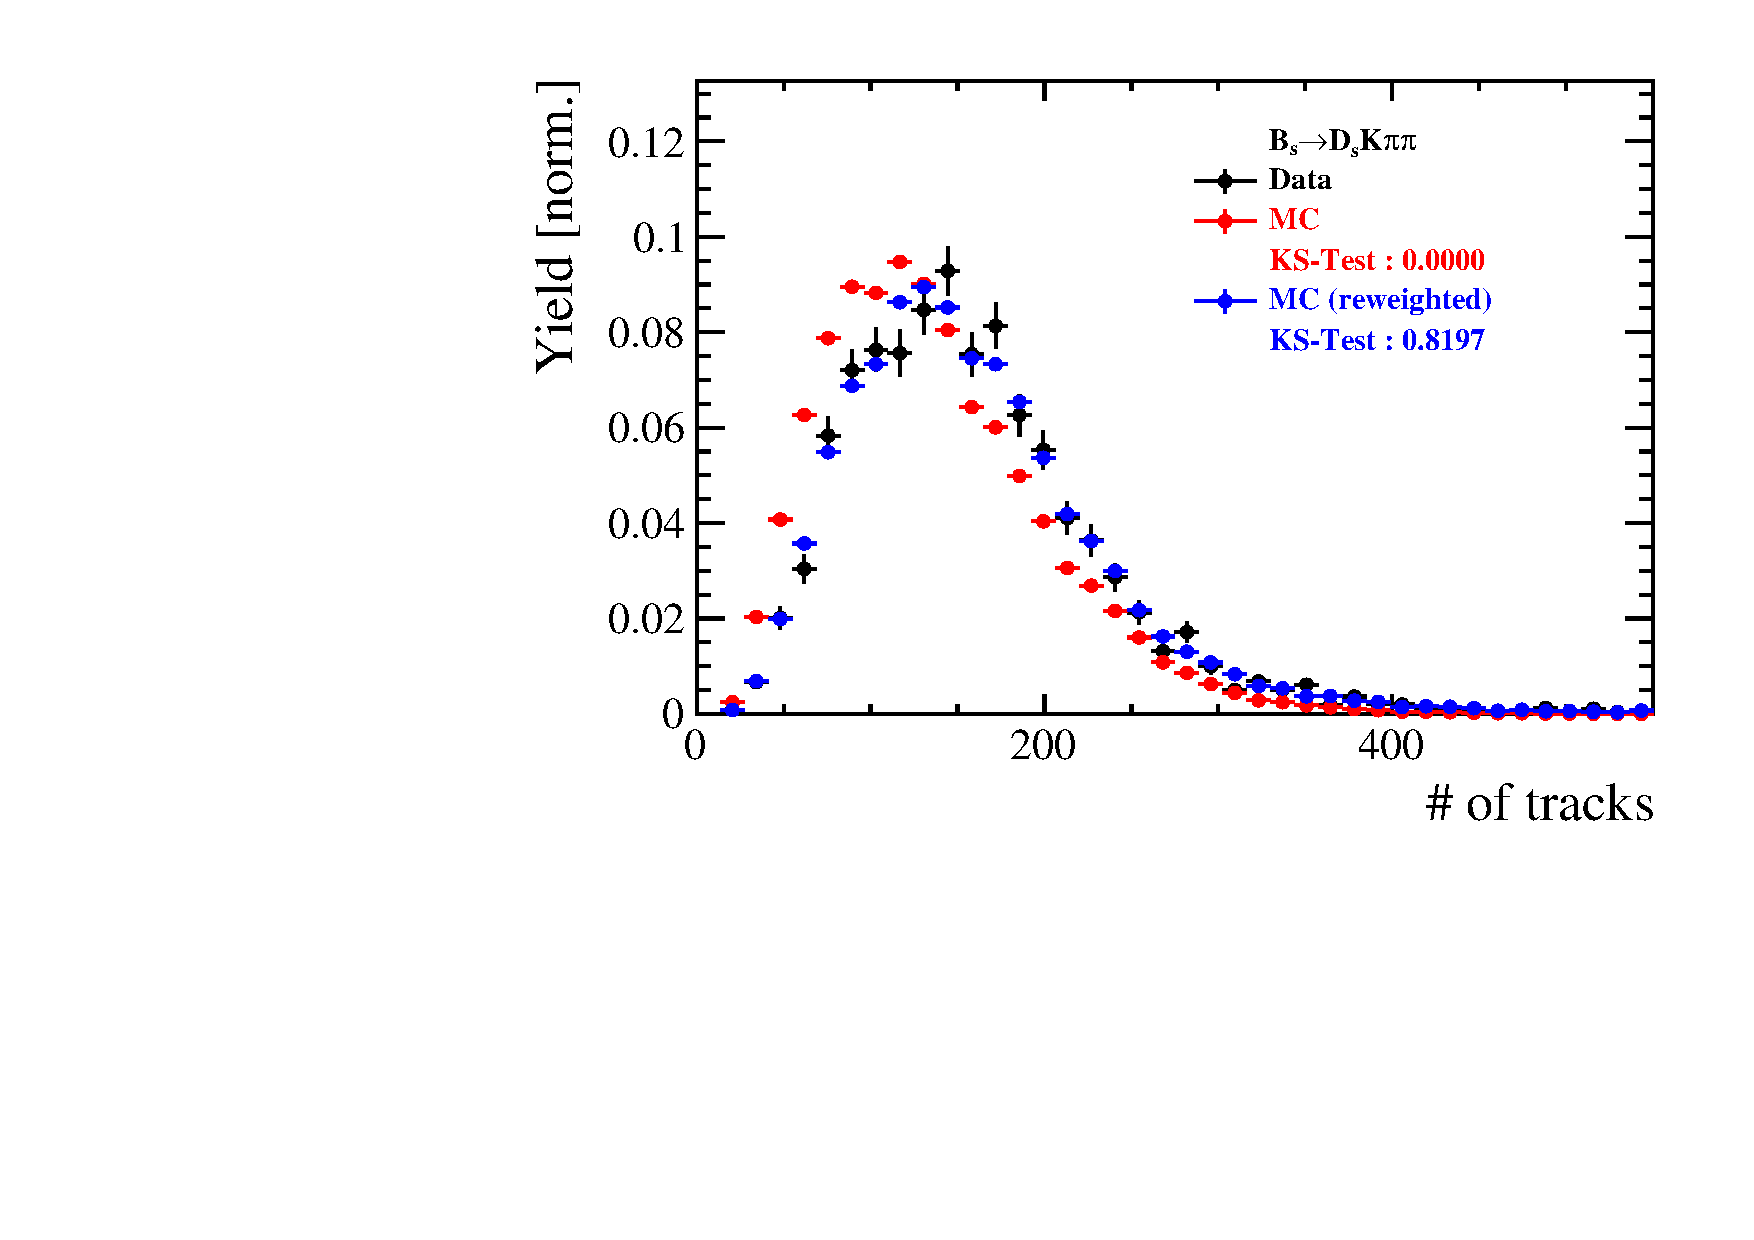
\includegraphics[height=!,width=0.3\textwidth]{figs/dataVsMC/signal_final/combined/Ds2all_NTracks.pdf}

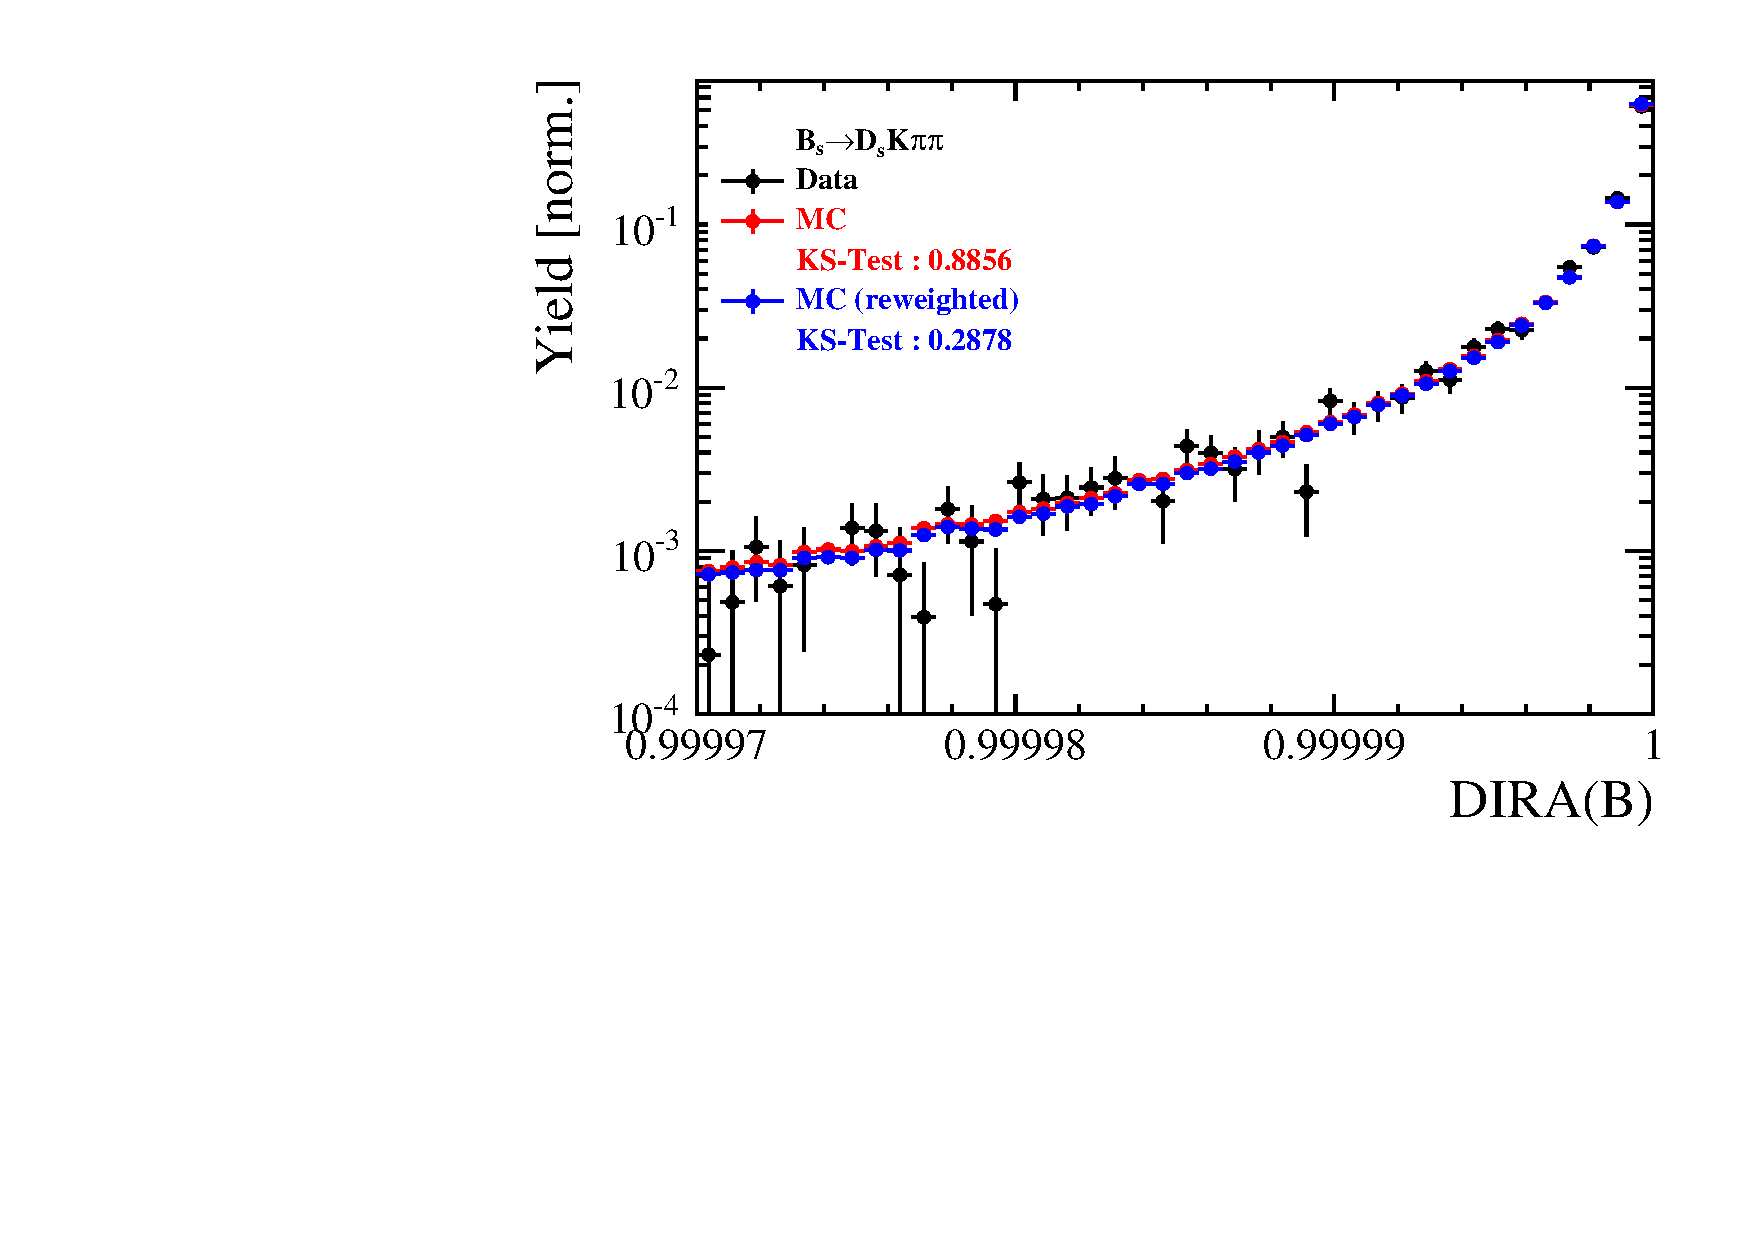
\includegraphics[height=!,width=0.3\textwidth]{figs/dataVsMC/signal_final/combined/Ds2all_Bs_DIRA_OWNPV.pdf}
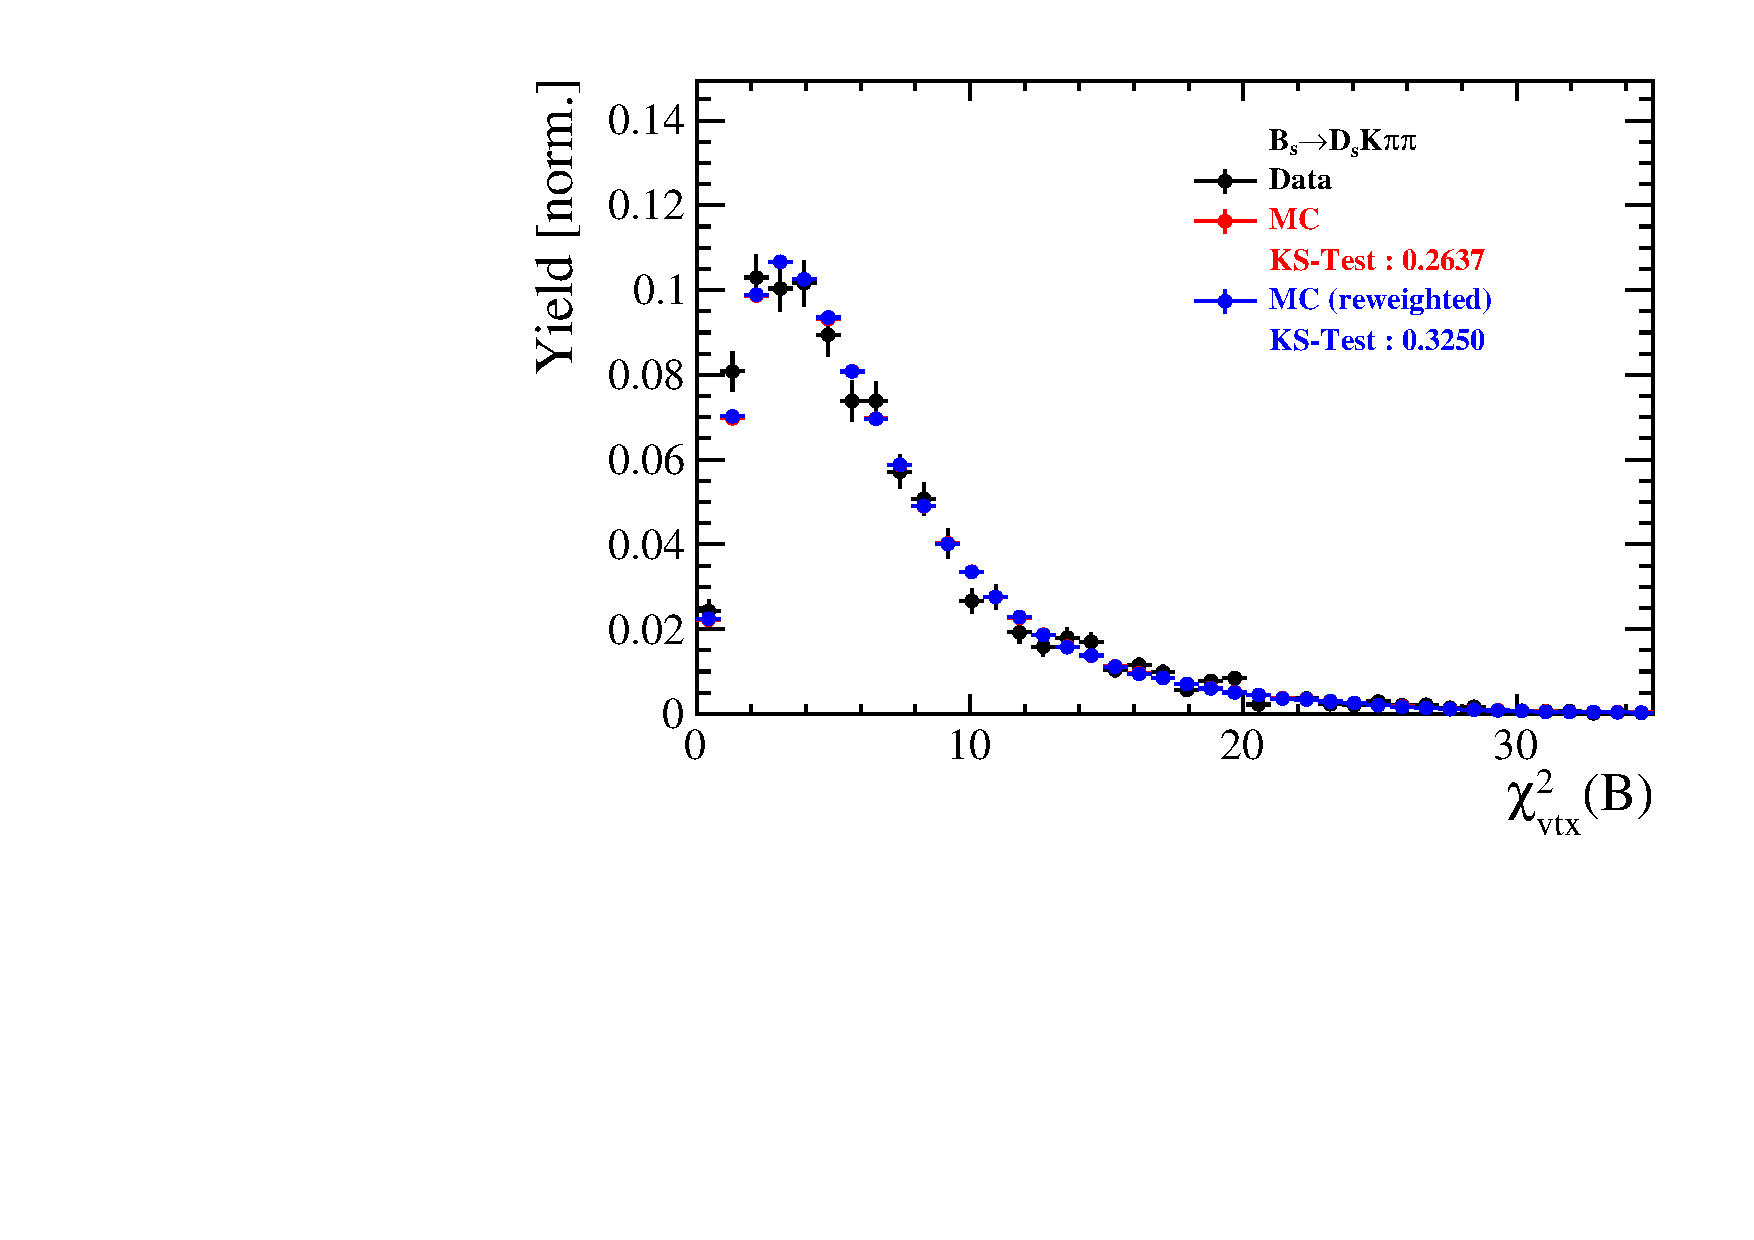
\includegraphics[height=!,width=0.3\textwidth]{figs/dataVsMC/signal_final/combined/Ds2all_Bs_ENDVERTEX_CHI2.pdf}
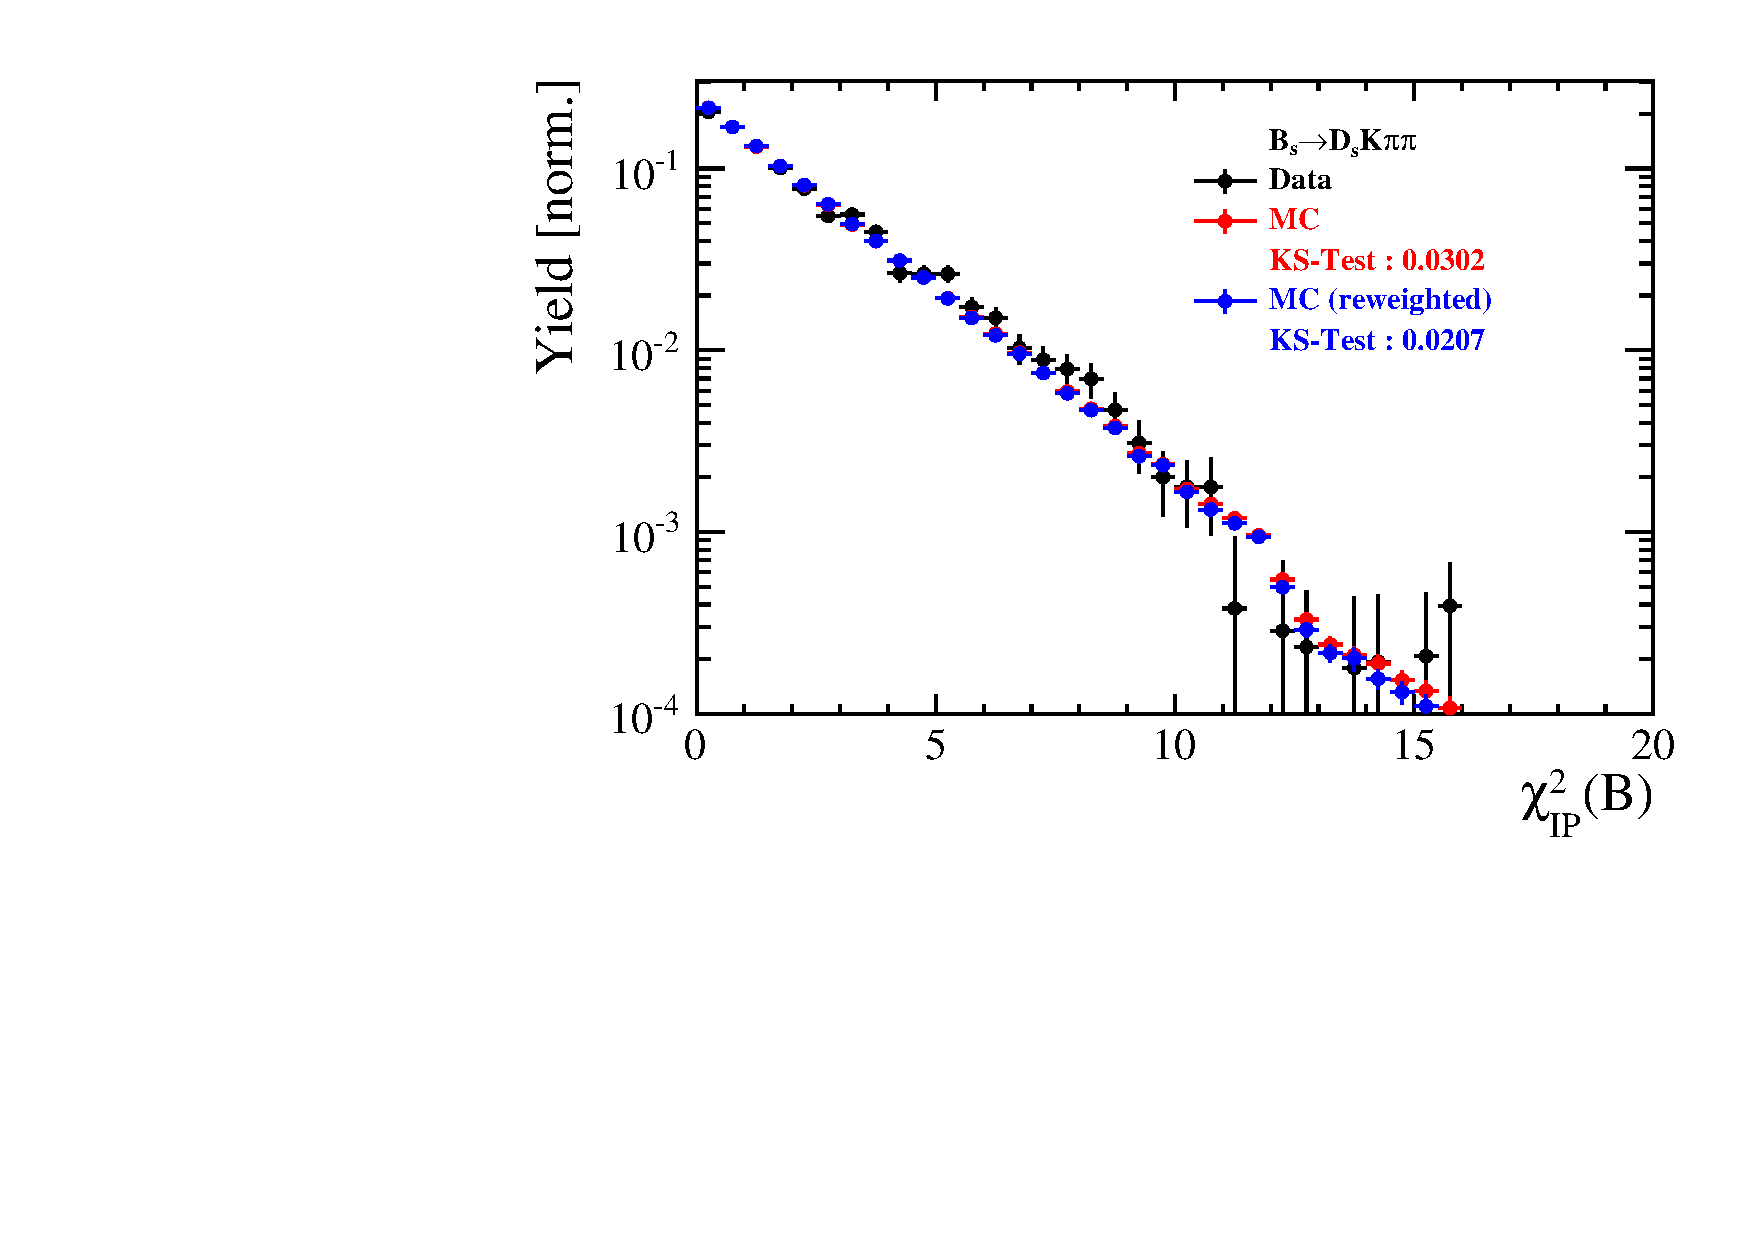
\includegraphics[height=!,width=0.3\textwidth]{figs/dataVsMC/signal_final/combined/Ds2all_Bs_IPCHI2_OWNPV.pdf}

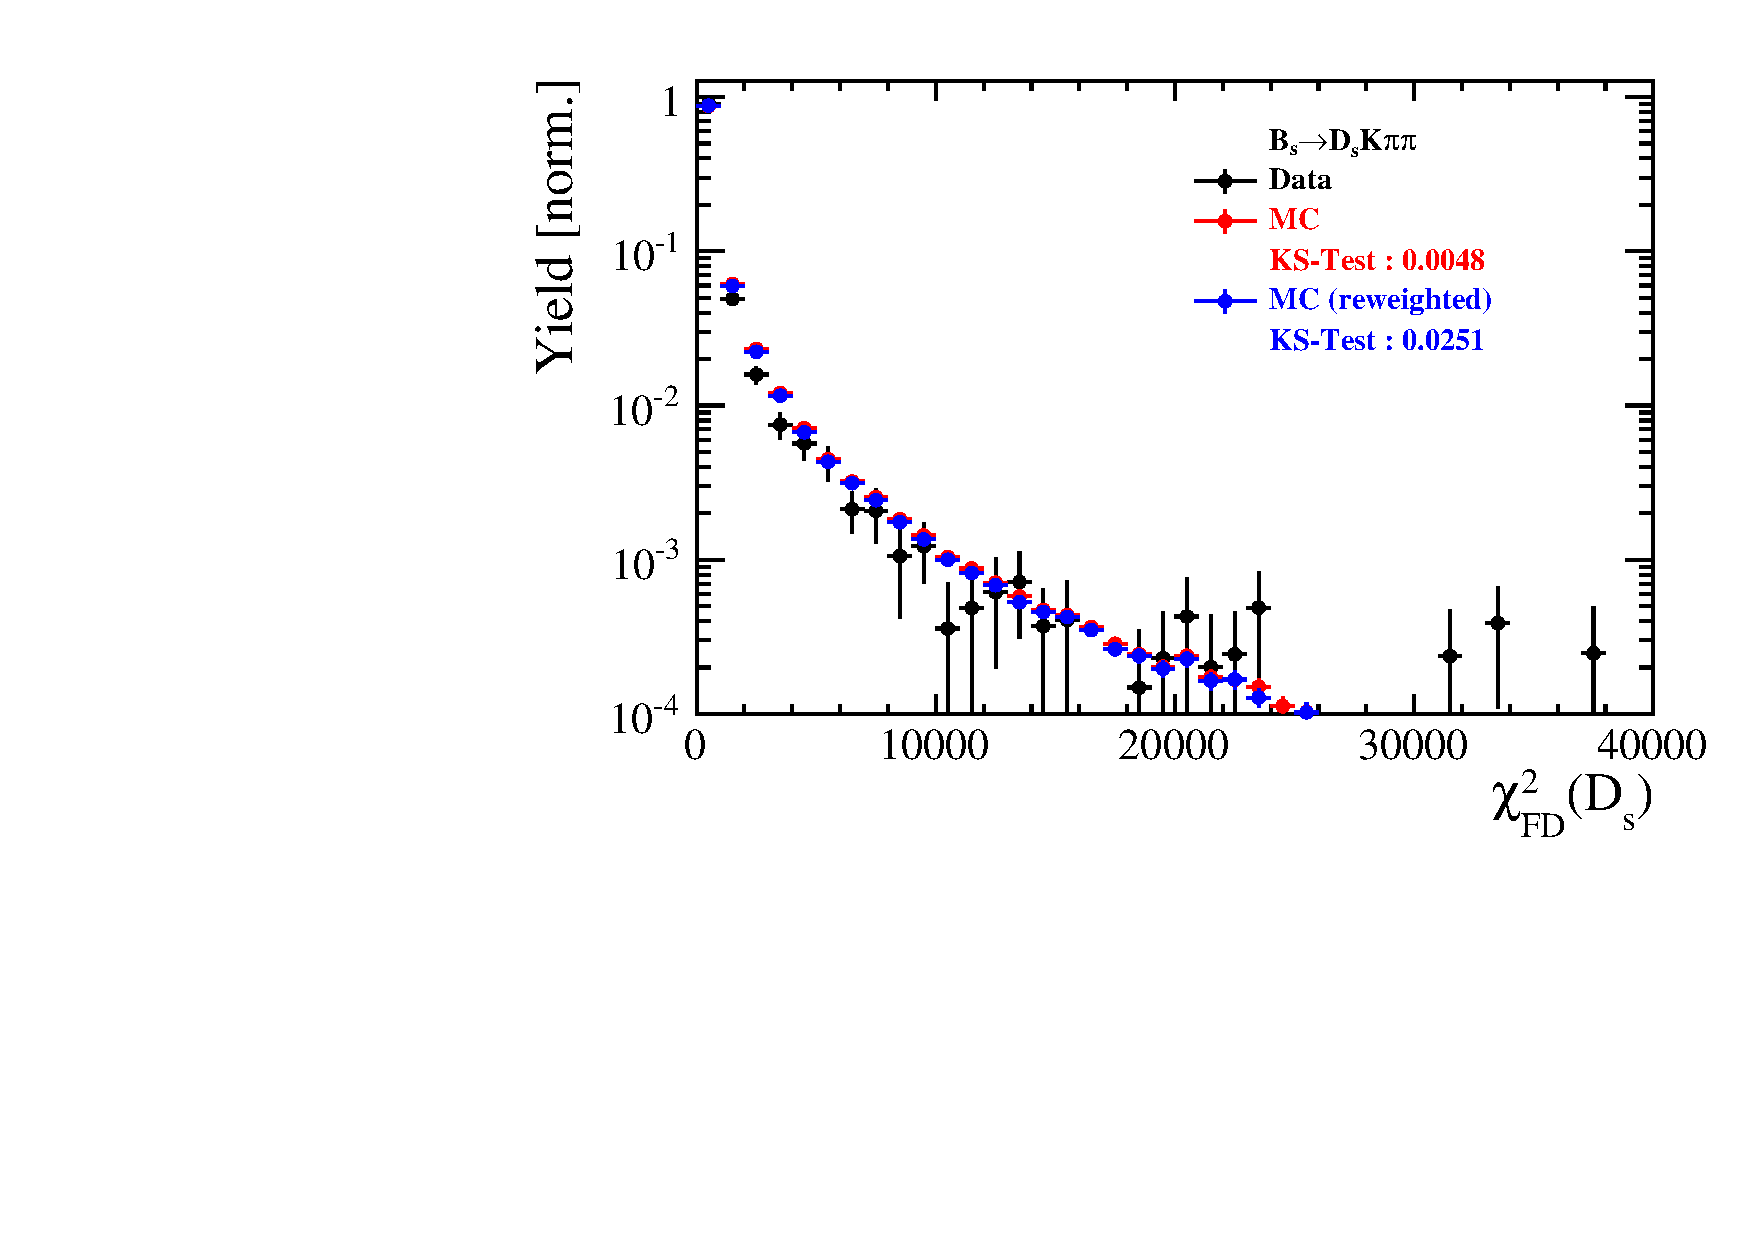
\includegraphics[height=!,width=0.3\textwidth]{figs/dataVsMC/signal_final/combined/Ds2all_Ds_FDCHI2_ORIVX.pdf}
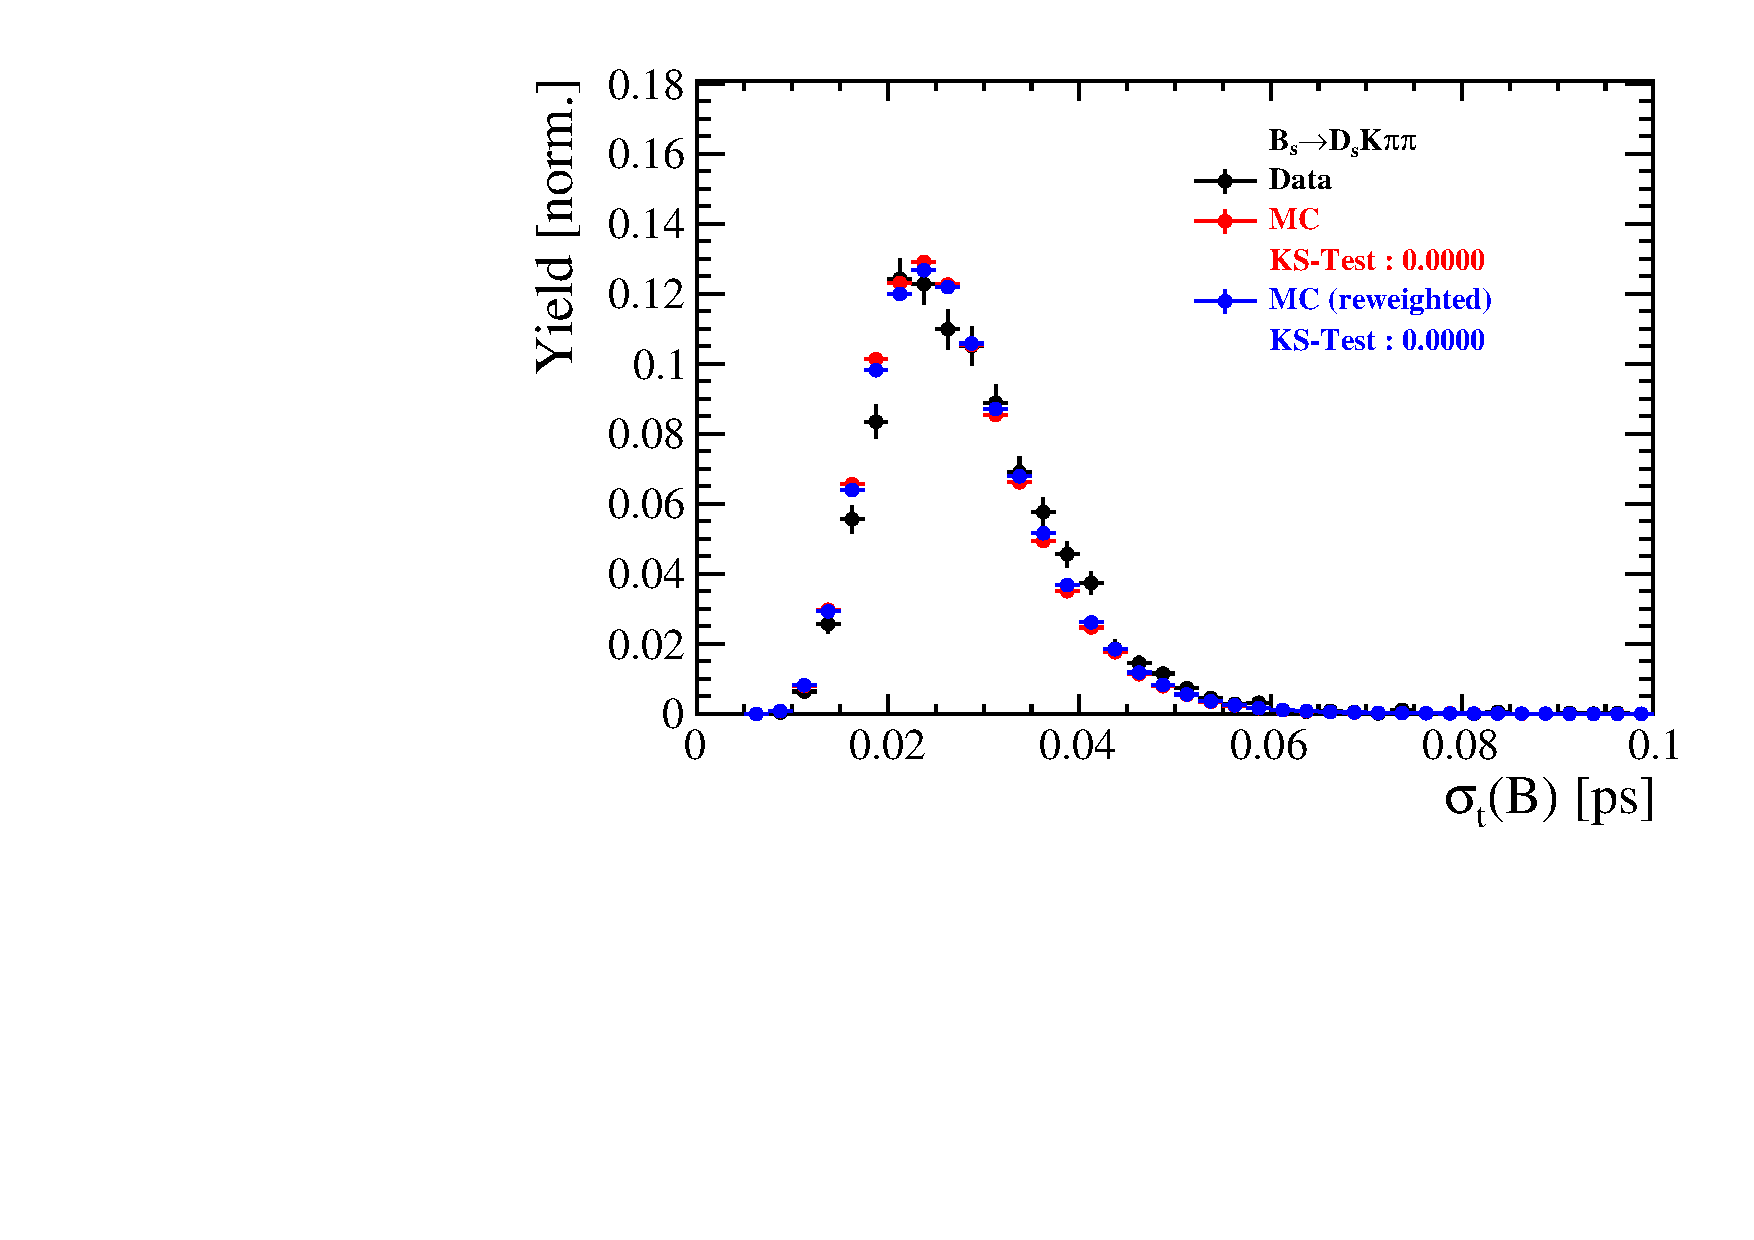
\includegraphics[height=!,width=0.3\textwidth]{figs/dataVsMC/signal_final/combined/Ds2all_Bs_BsDTF_TAUERR.pdf}
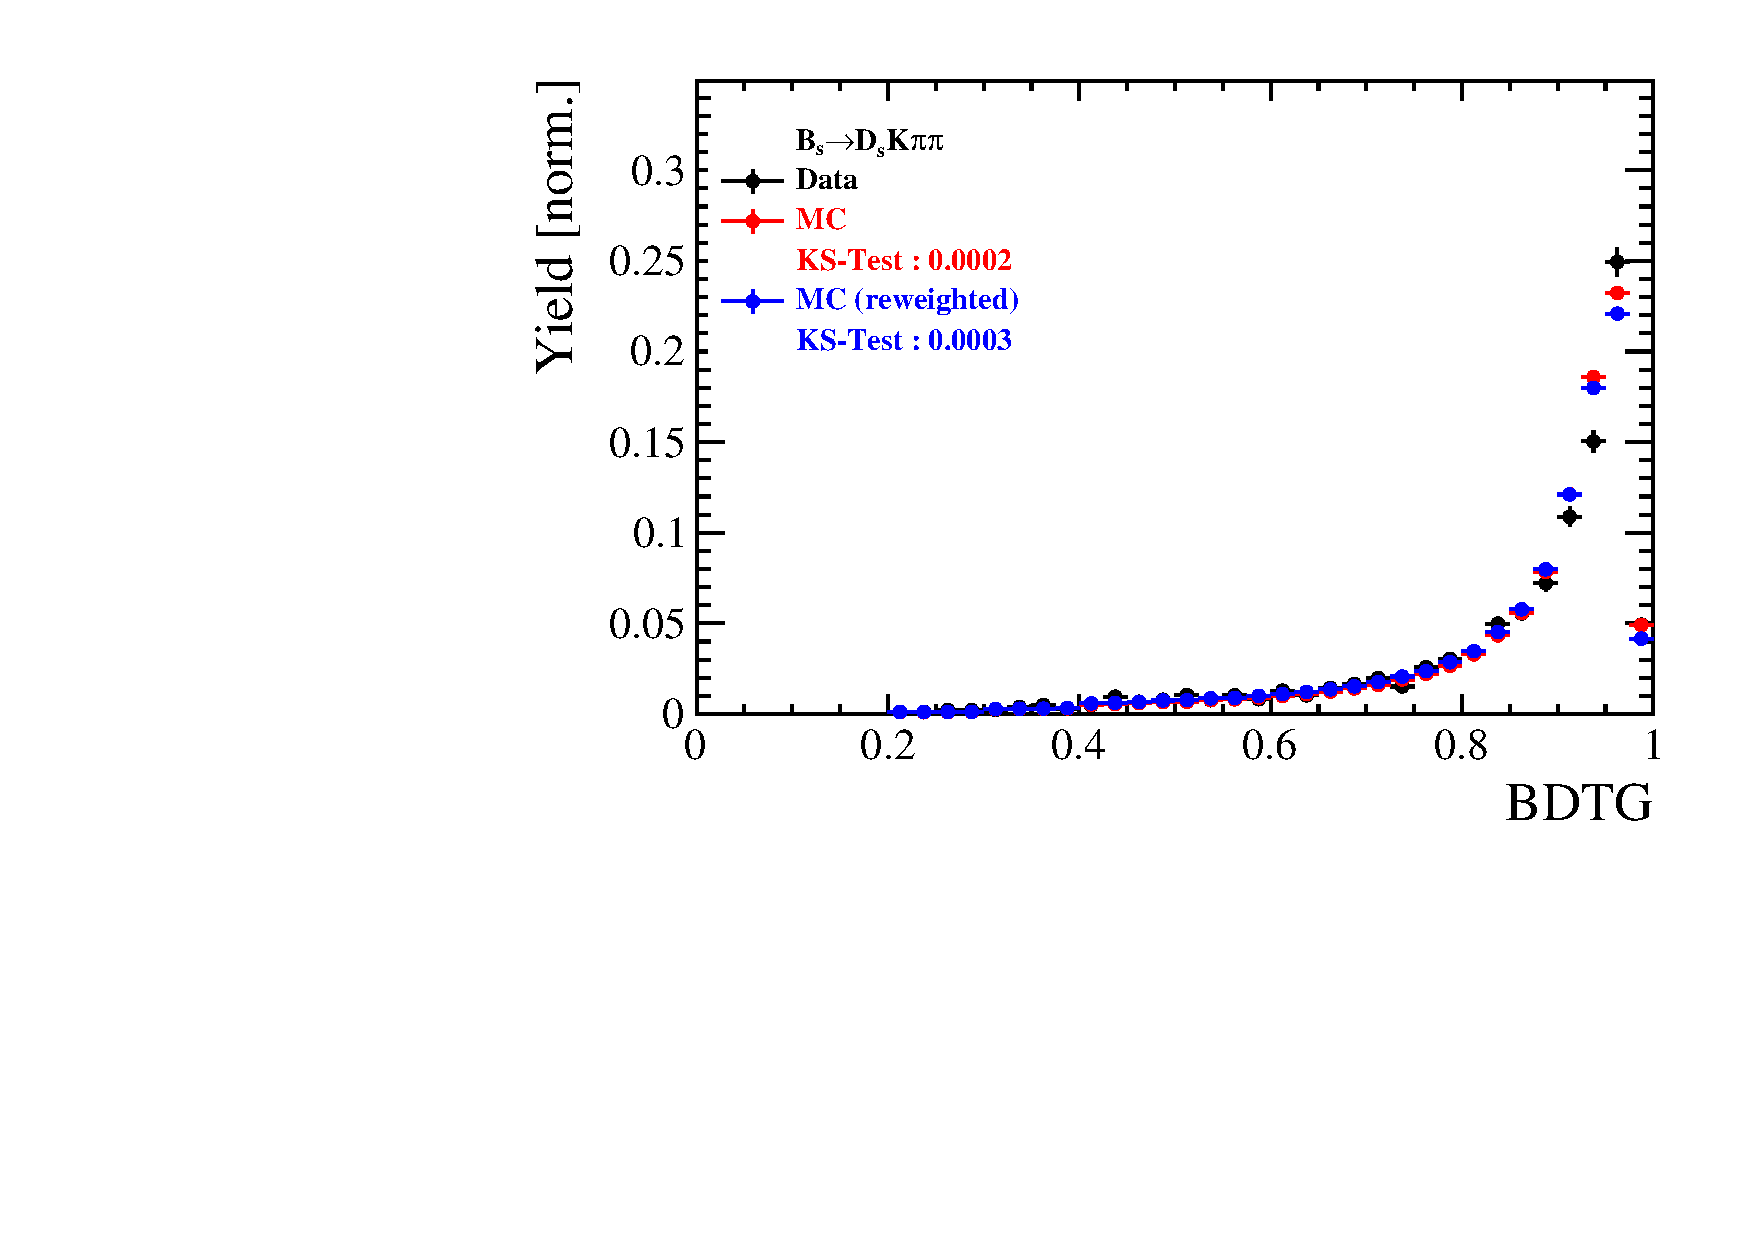
\includegraphics[height=!,width=0.3\textwidth]{figs/dataVsMC/signal_final/combined/Ds2all_BDTG_response.pdf}

%
%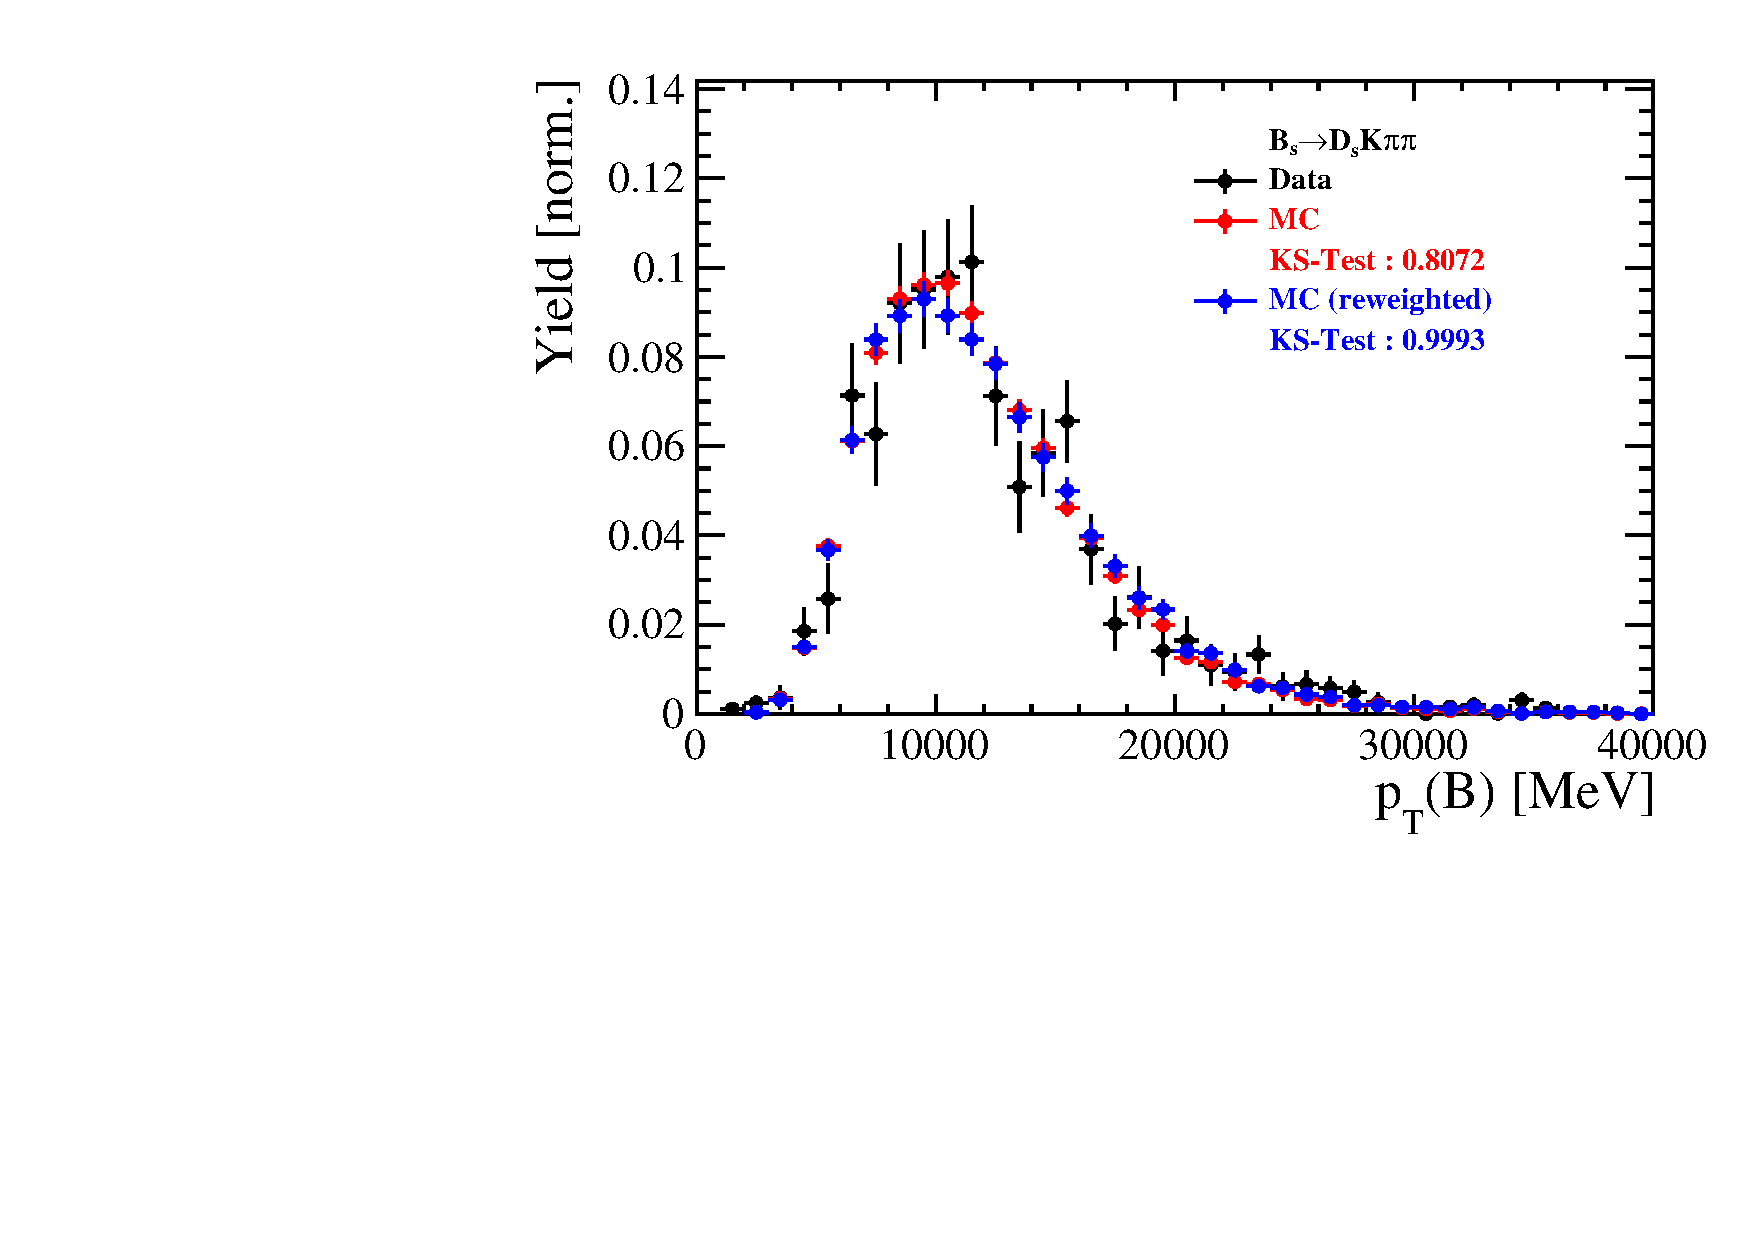
\includegraphics[height=!,width=0.4\textwidth]{figs/dataVsMC/signal_final/combined/Ds2KKpi_1_Bs_PT.pdf}
%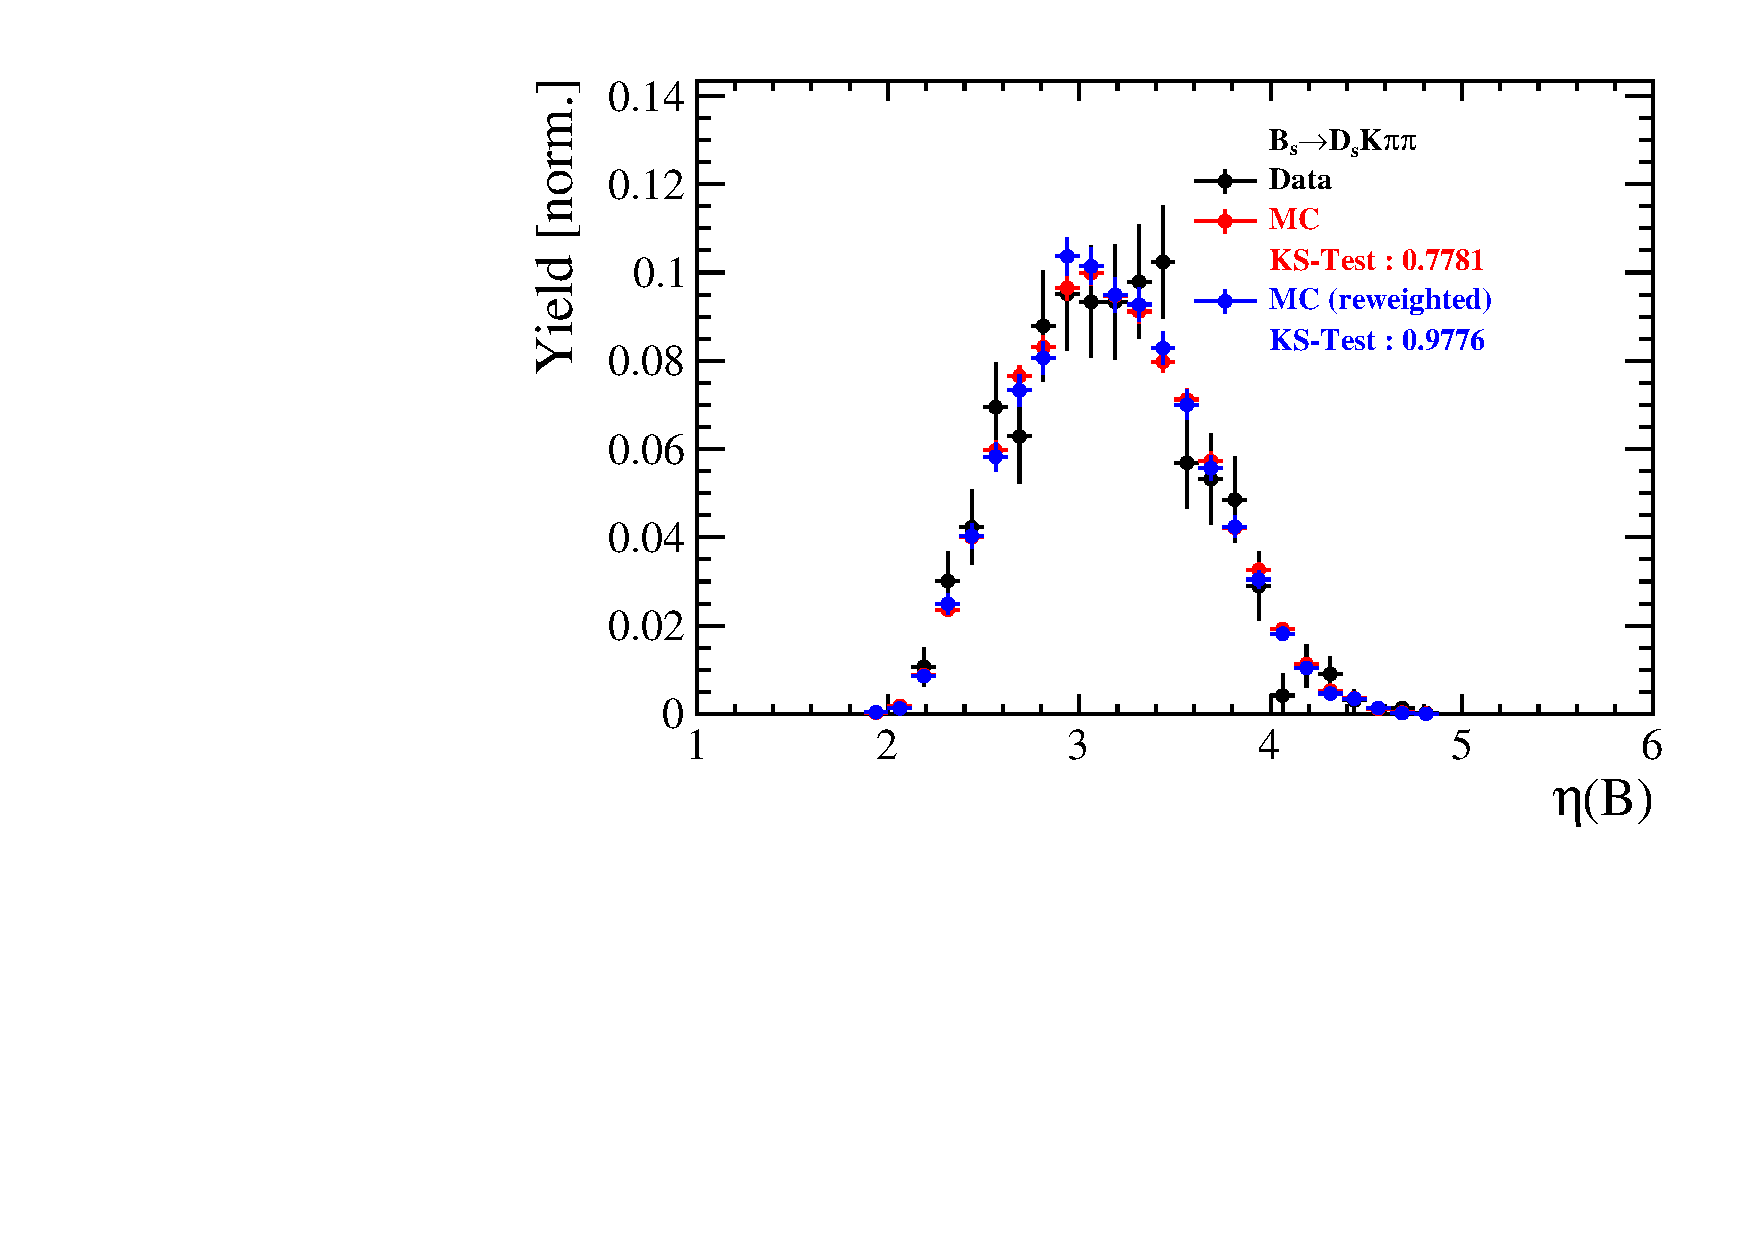
\includegraphics[height=!,width=0.4\textwidth]{figs/dataVsMC/signal_final/combined/Ds2KKpi_1_Bs_ETA.pdf}
%
%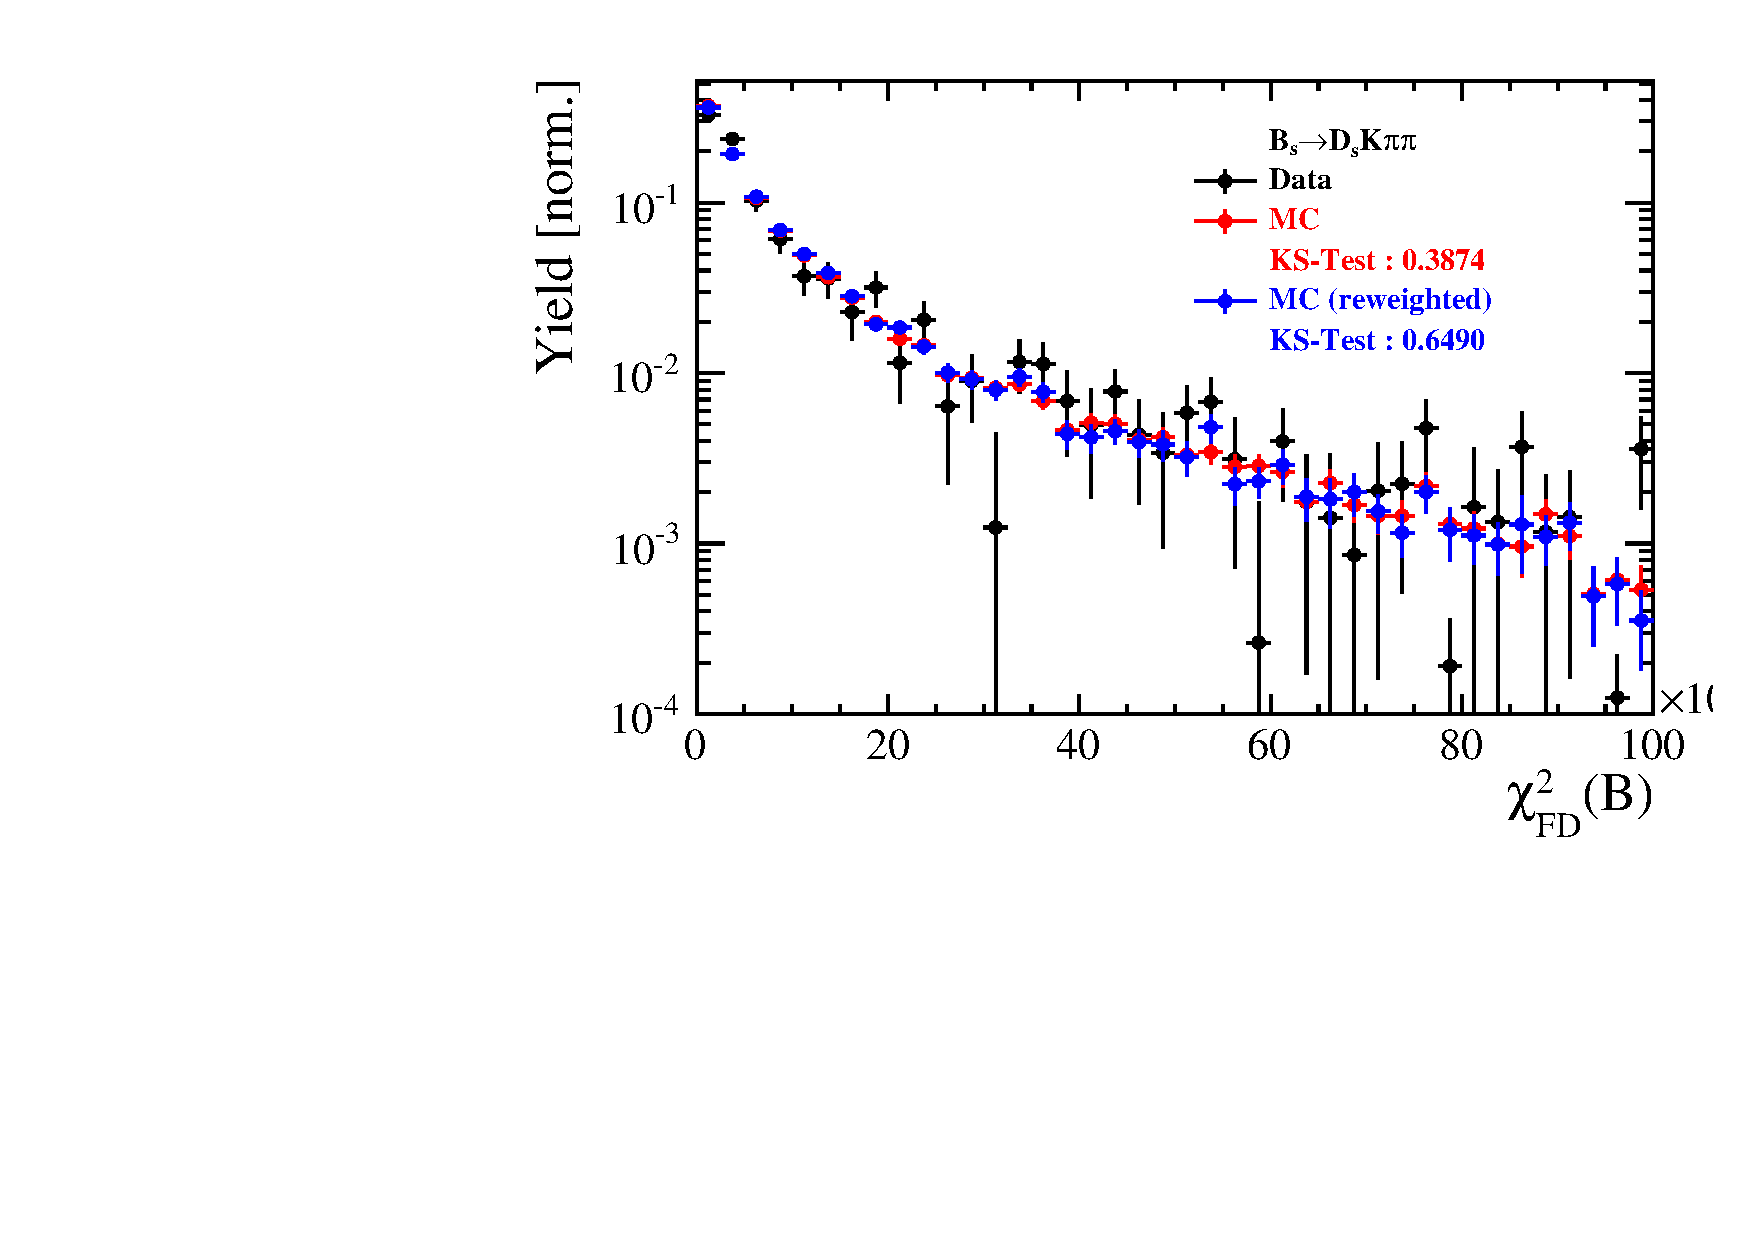
\includegraphics[height=!,width=0.4\textwidth]{figs/dataVsMC/signal_final/combined/Ds2KKpi_1_Bs_FDCHI2_OWNPV.pdf}
%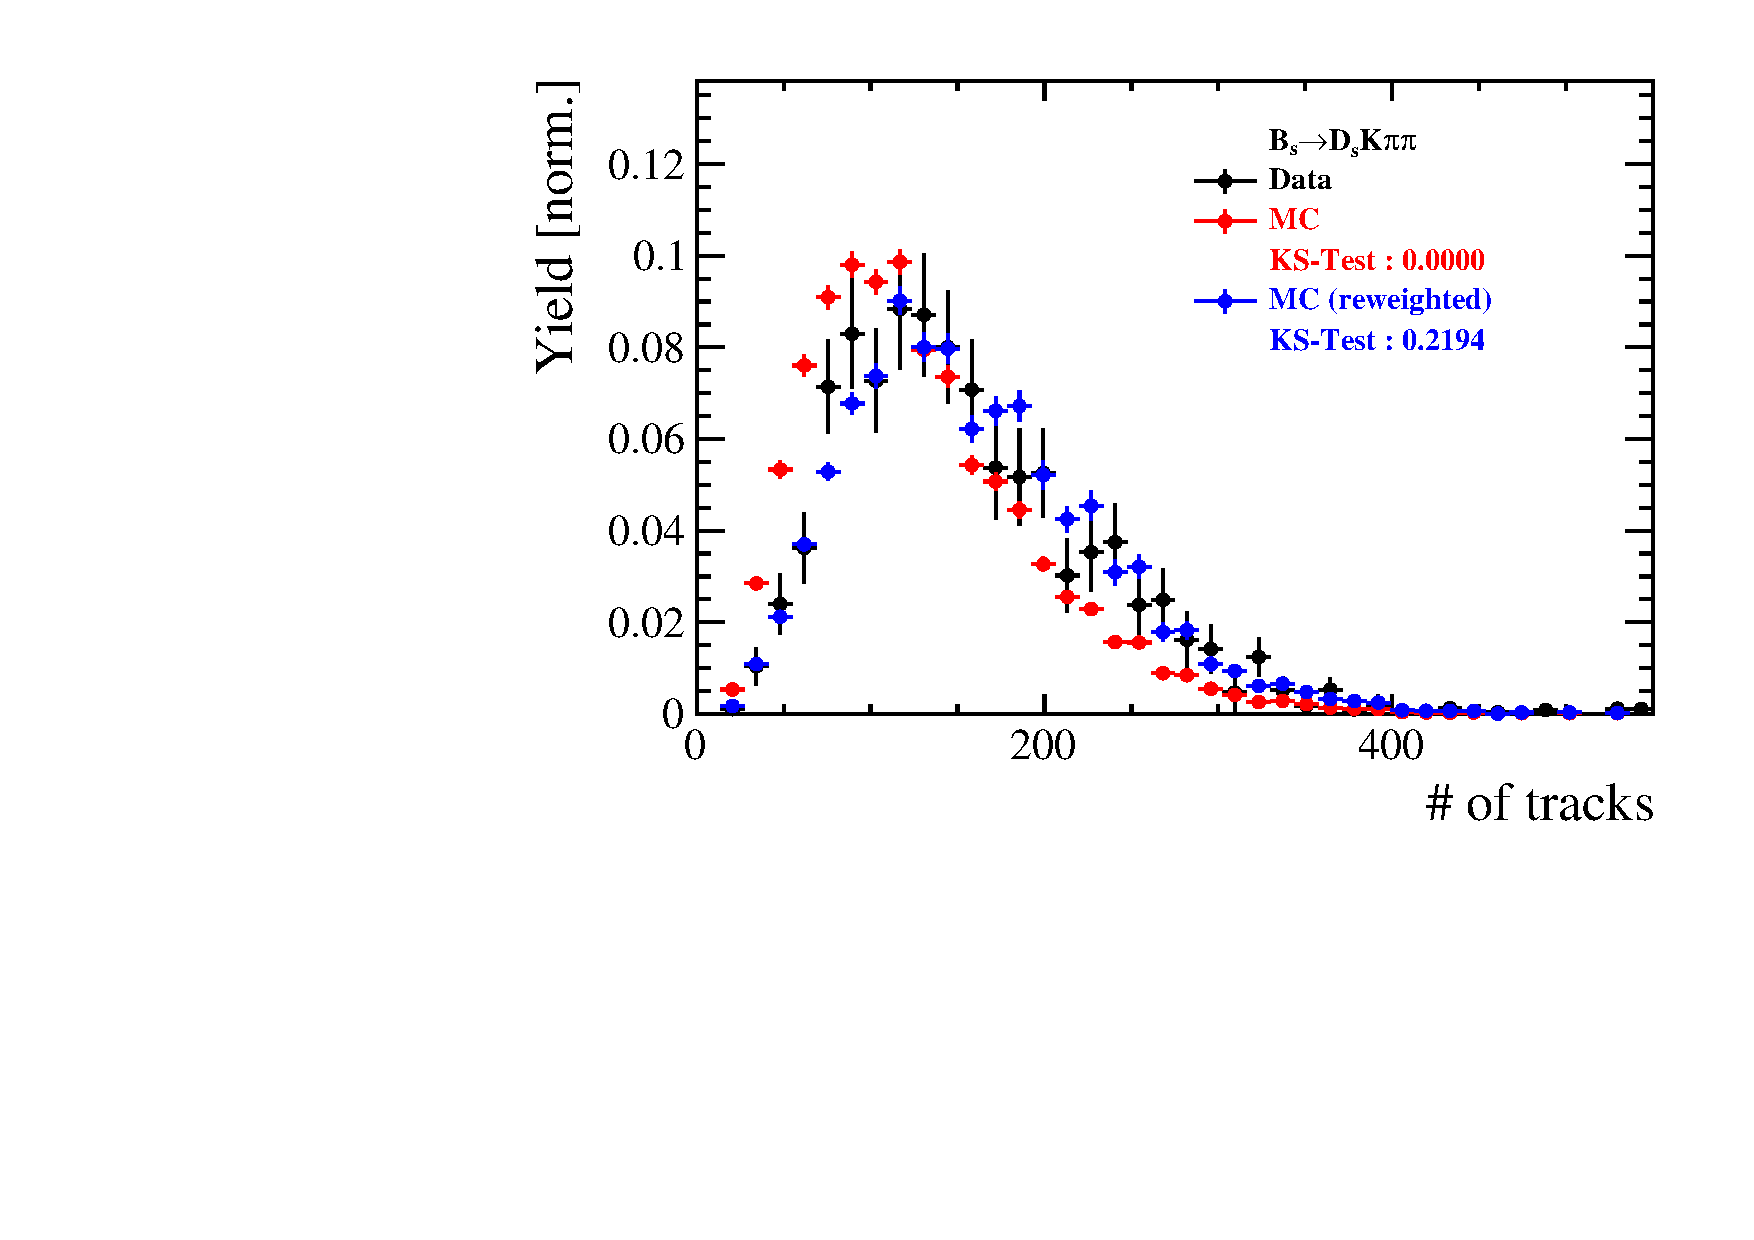
\includegraphics[height=!,width=0.4\textwidth]{figs/dataVsMC/signal_final/combined/Ds2KKpi_1_NTracks.pdf}
%
%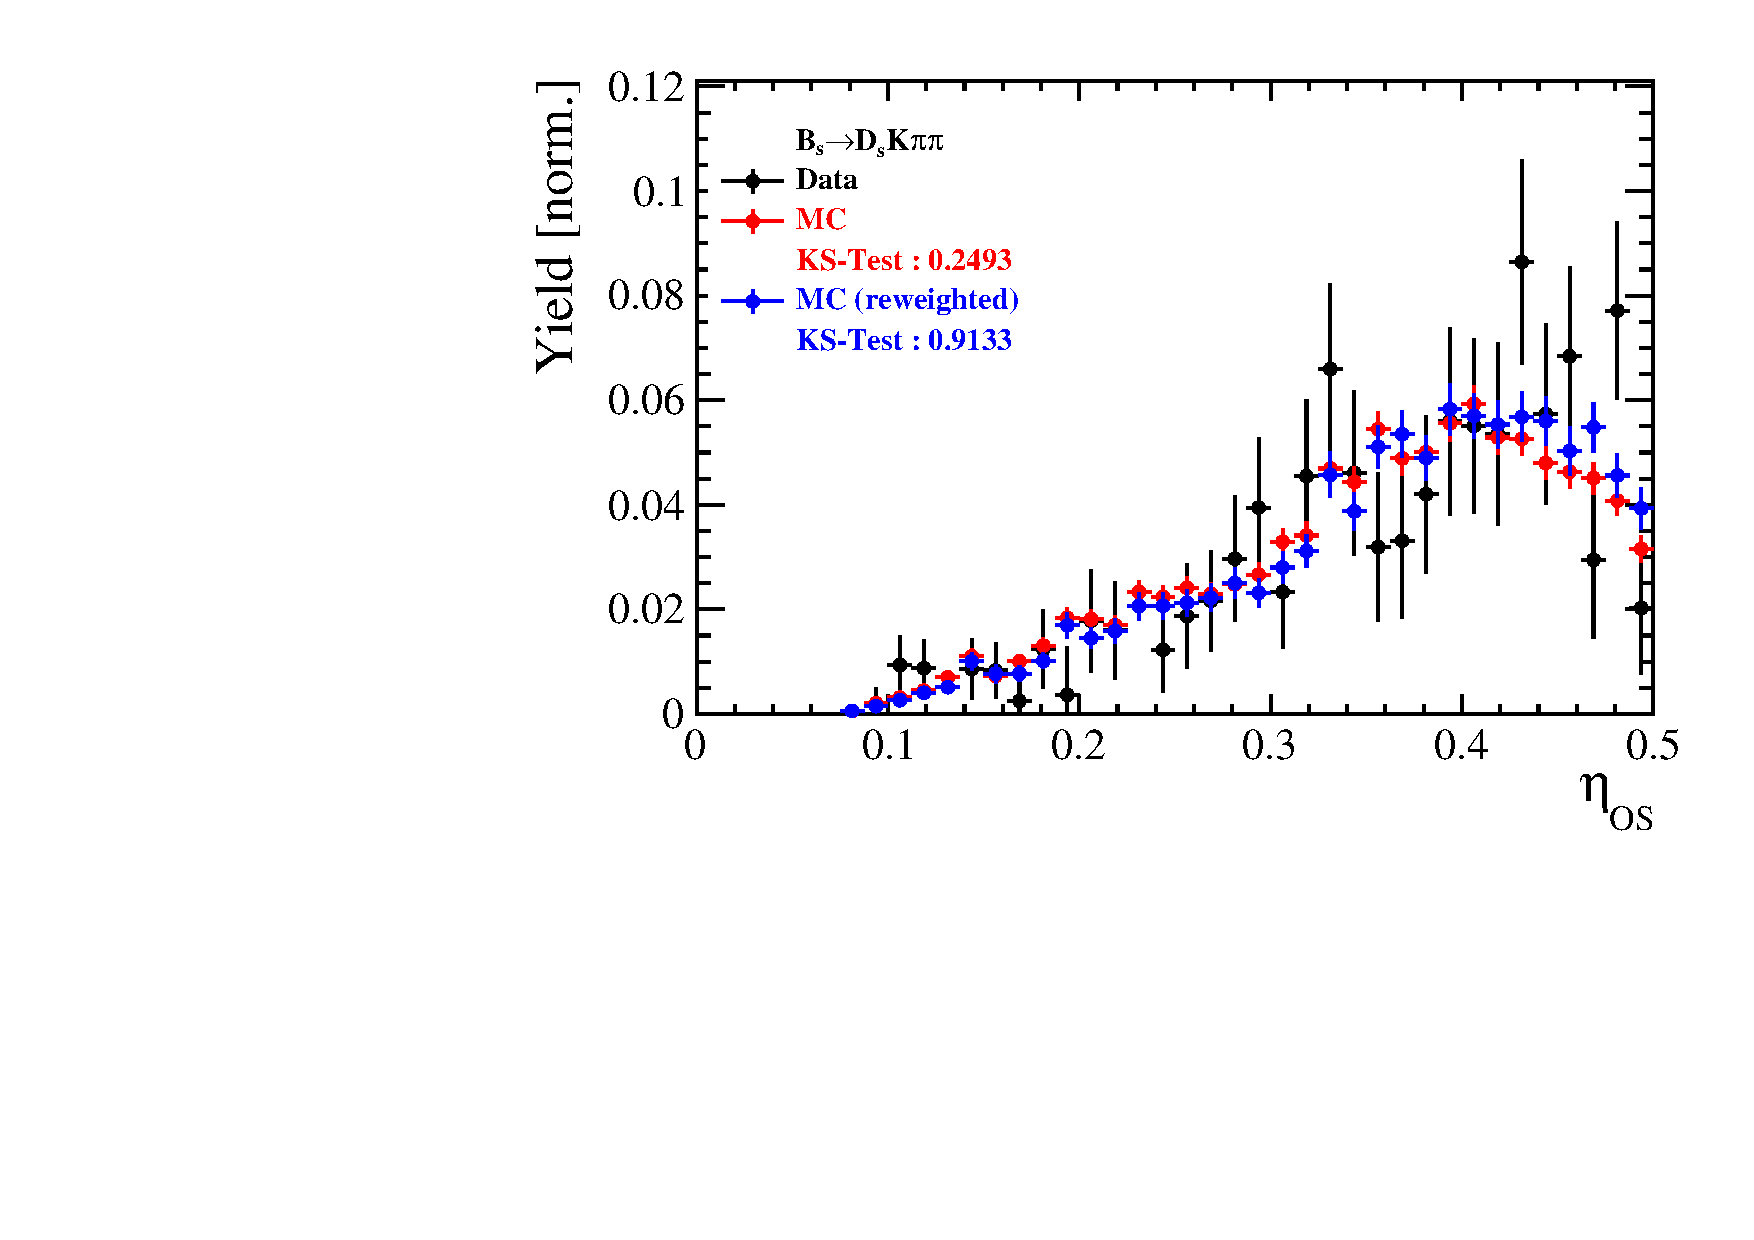
\includegraphics[height=!,width=0.4\textwidth]{figs/dataVsMC/signal_final/combined/Ds2KKpi_1_Bs_TAGOMEGA_OS.pdf}
%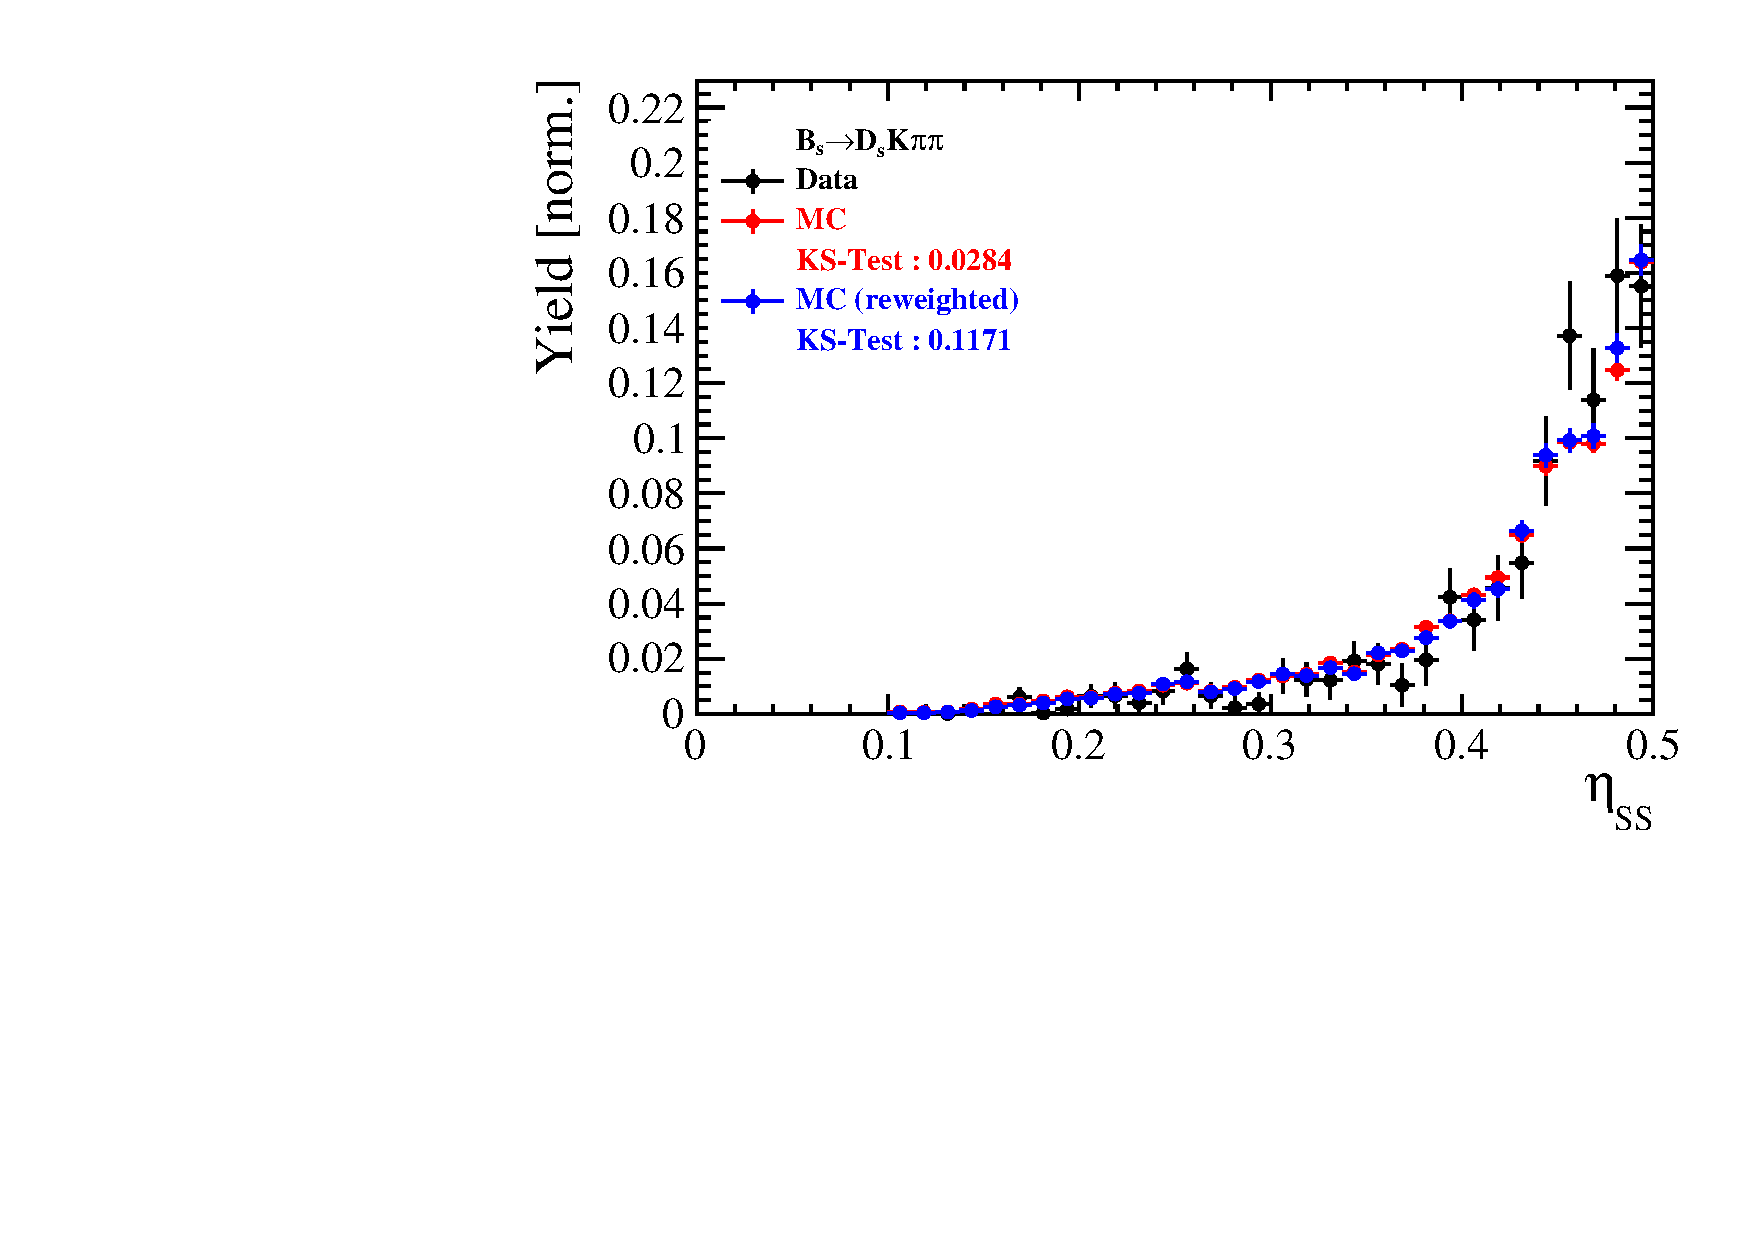
\includegraphics[height=!,width=0.4\textwidth]{figs/dataVsMC/signal_final/combined/Ds2KKpi_1_Bs_SS_nnetKaon_PROB.pdf}
%
%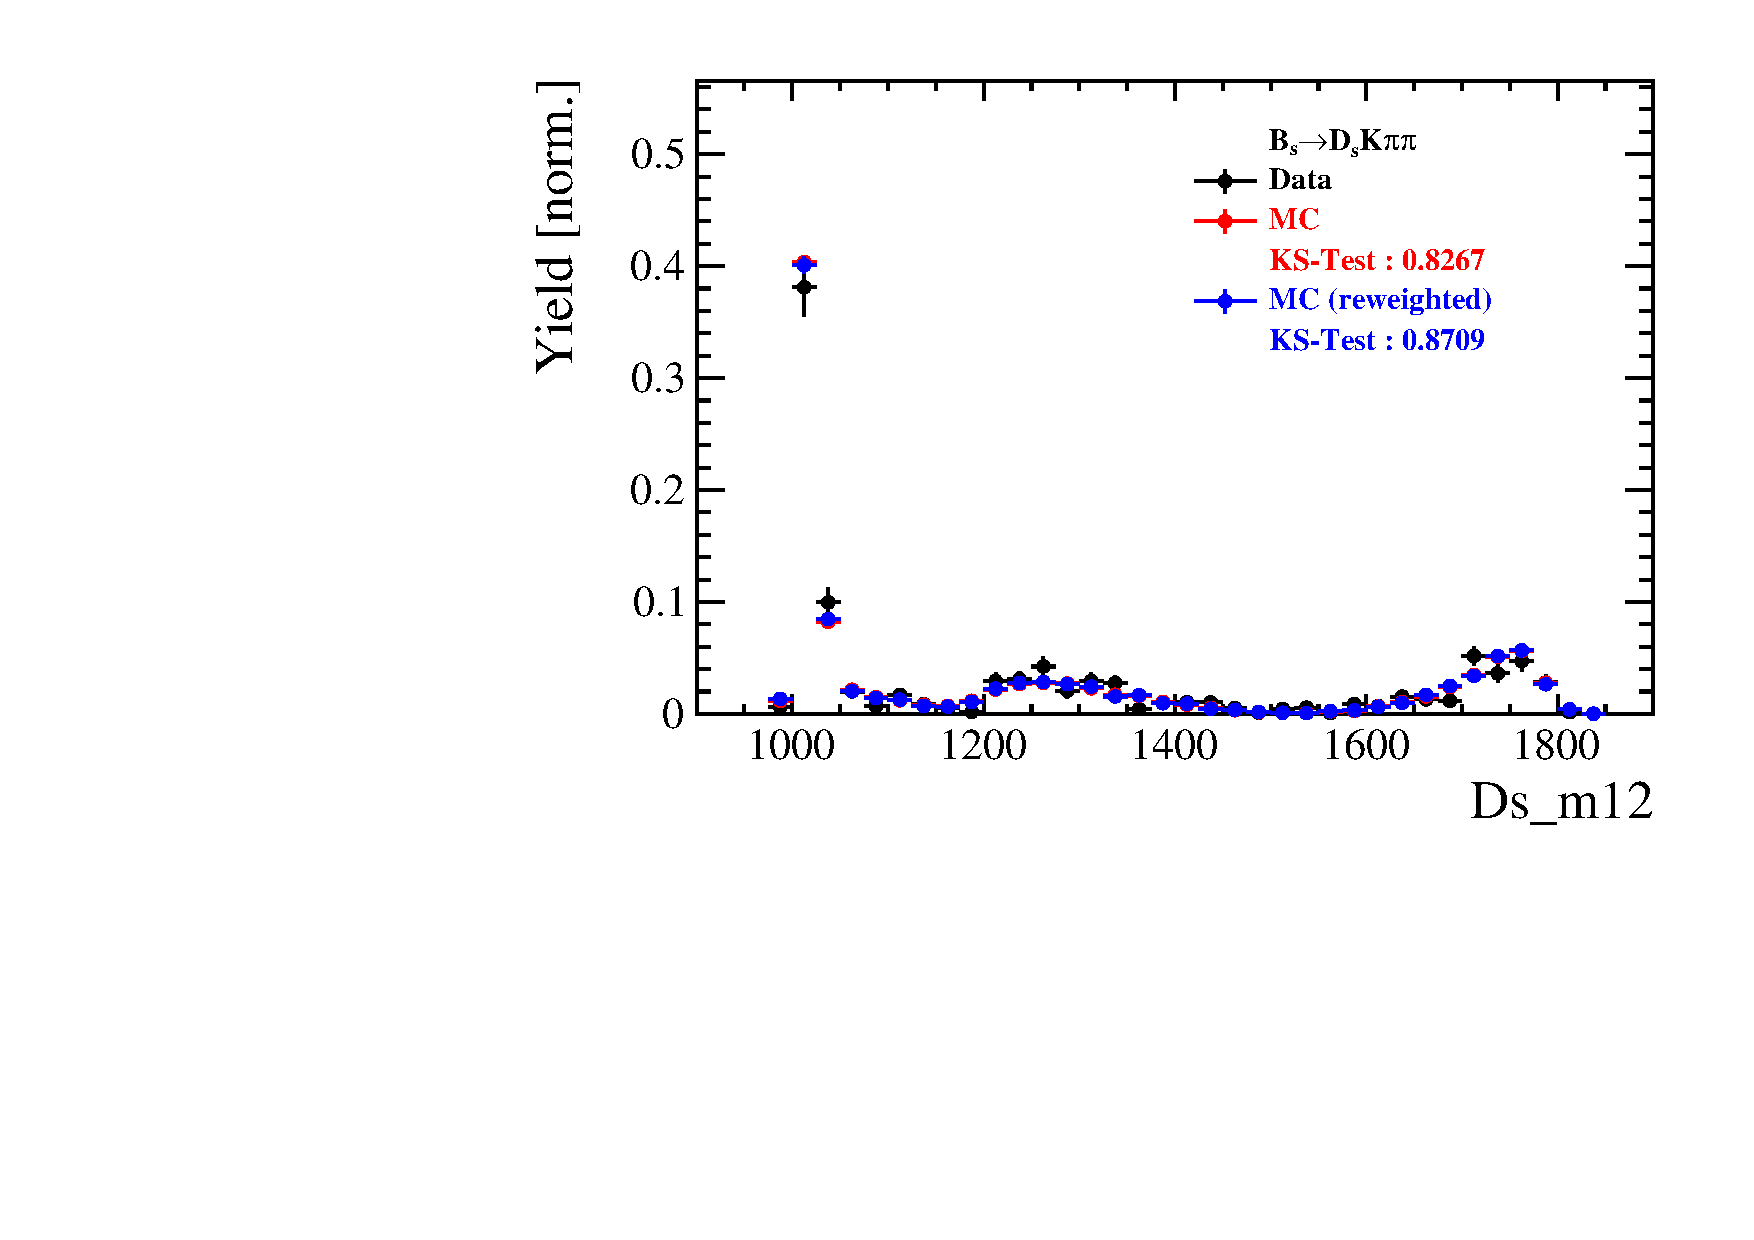
\includegraphics[height=!,width=0.4\textwidth]{figs/dataVsMC/signal_final/combined/Ds2KKpi_1_Ds_m12.pdf}
%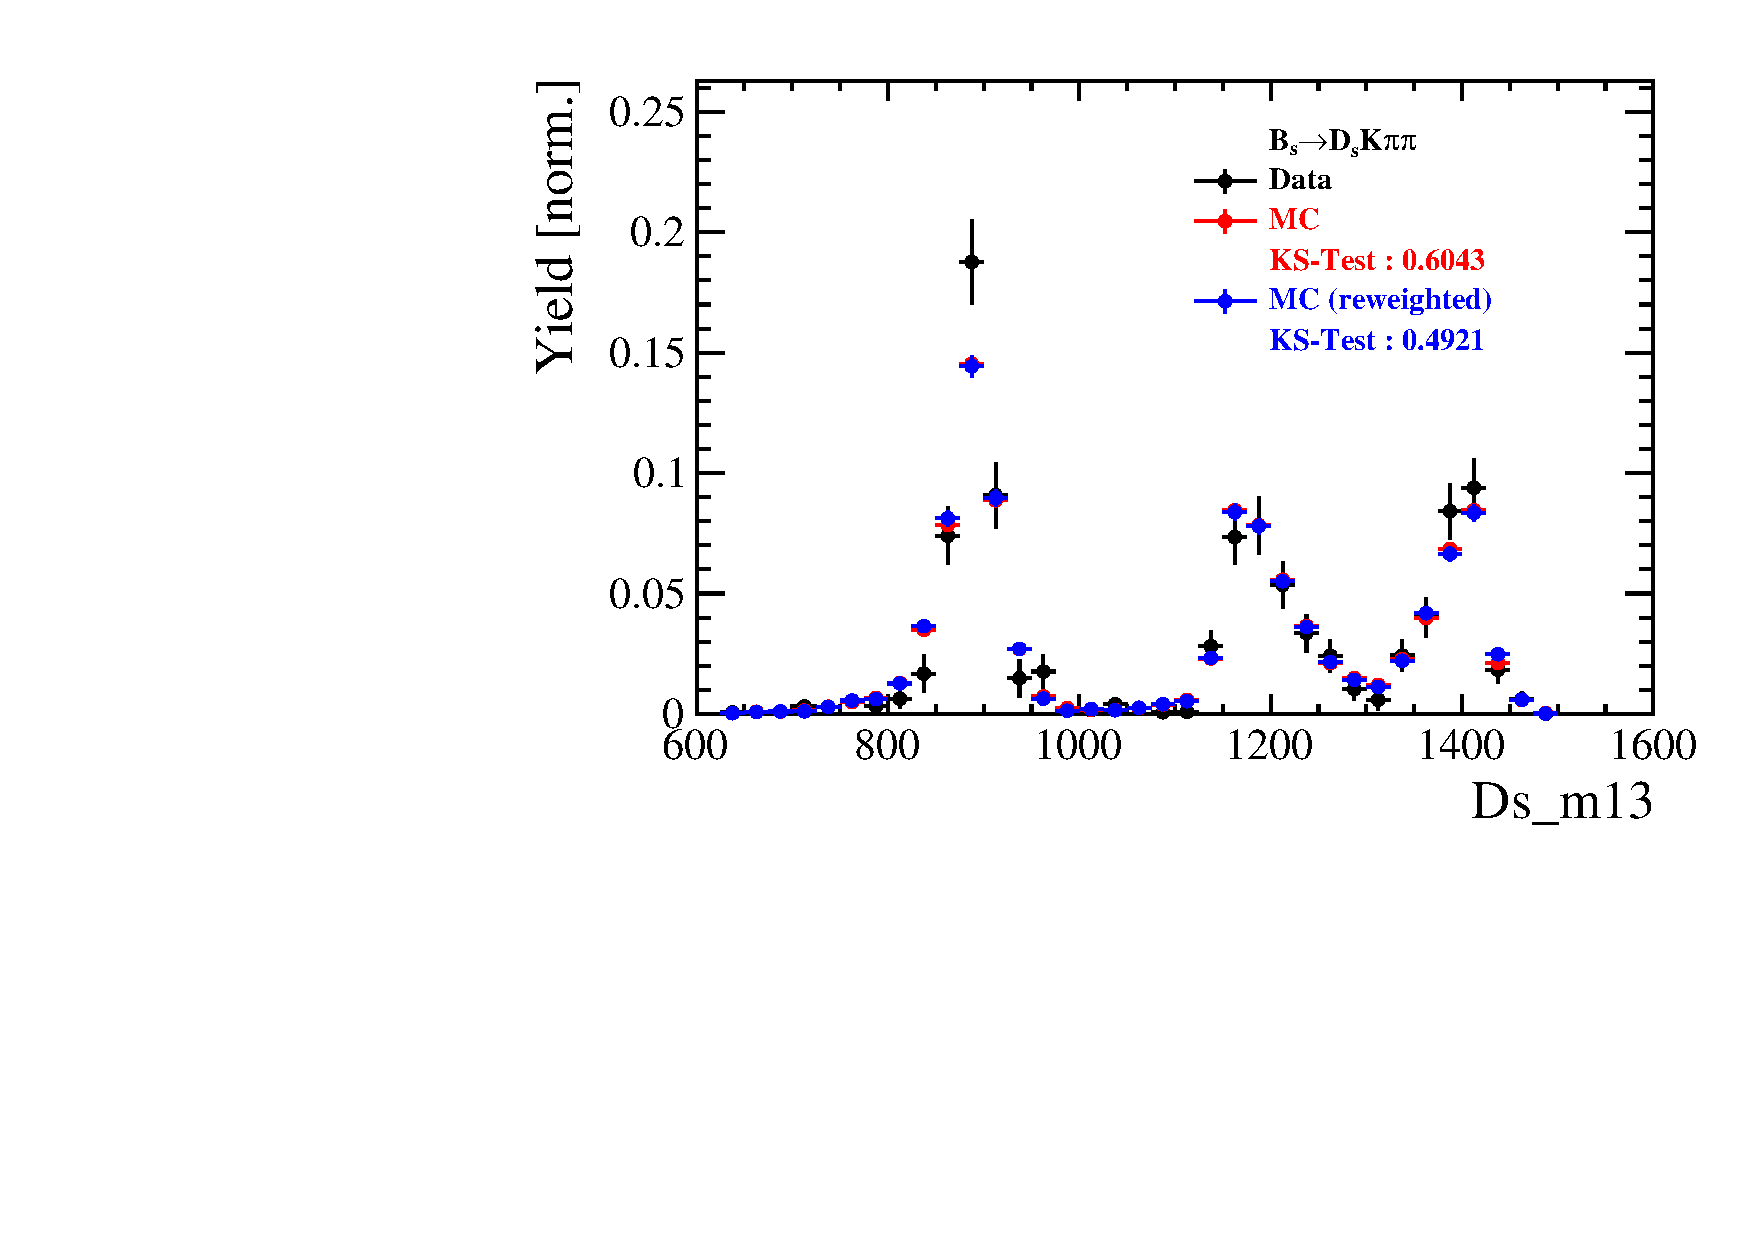
\includegraphics[height=!,width=0.4\textwidth]{figs/dataVsMC/signal_final/combined/Ds2KKpi_1_Ds_m13.pdf}

\caption{\footnotesize Comparison between data and MC of  selected variables for $B_s\to D_sK\pi\pi$ decays.}
\label{fig:}
\end{figure}
%
%\begin{figure}[h]
%\centering
%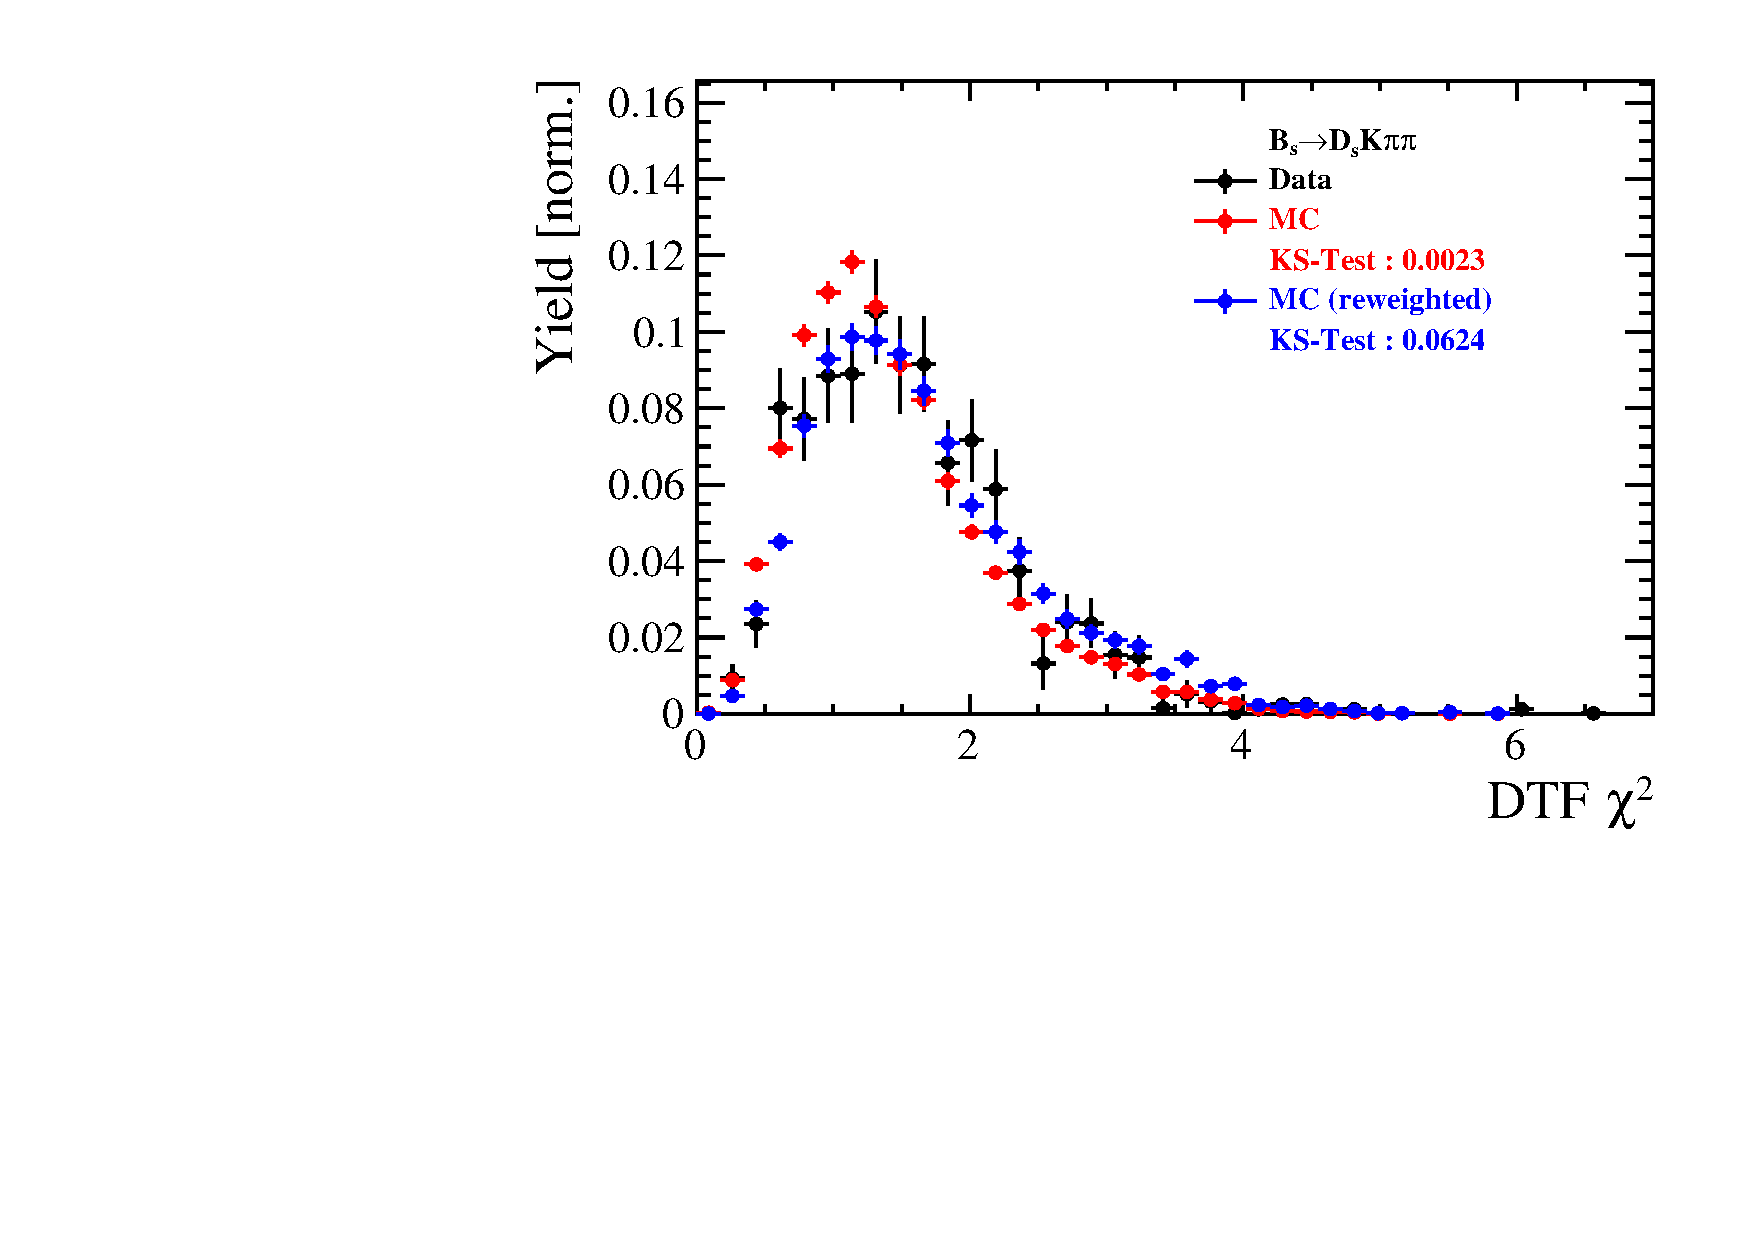
\includegraphics[height=!,width=0.4\textwidth]{figs/dataVsMC/signal_final/combined/Ds2KKpi_1_DTF_CHI2NDOF.pdf}
%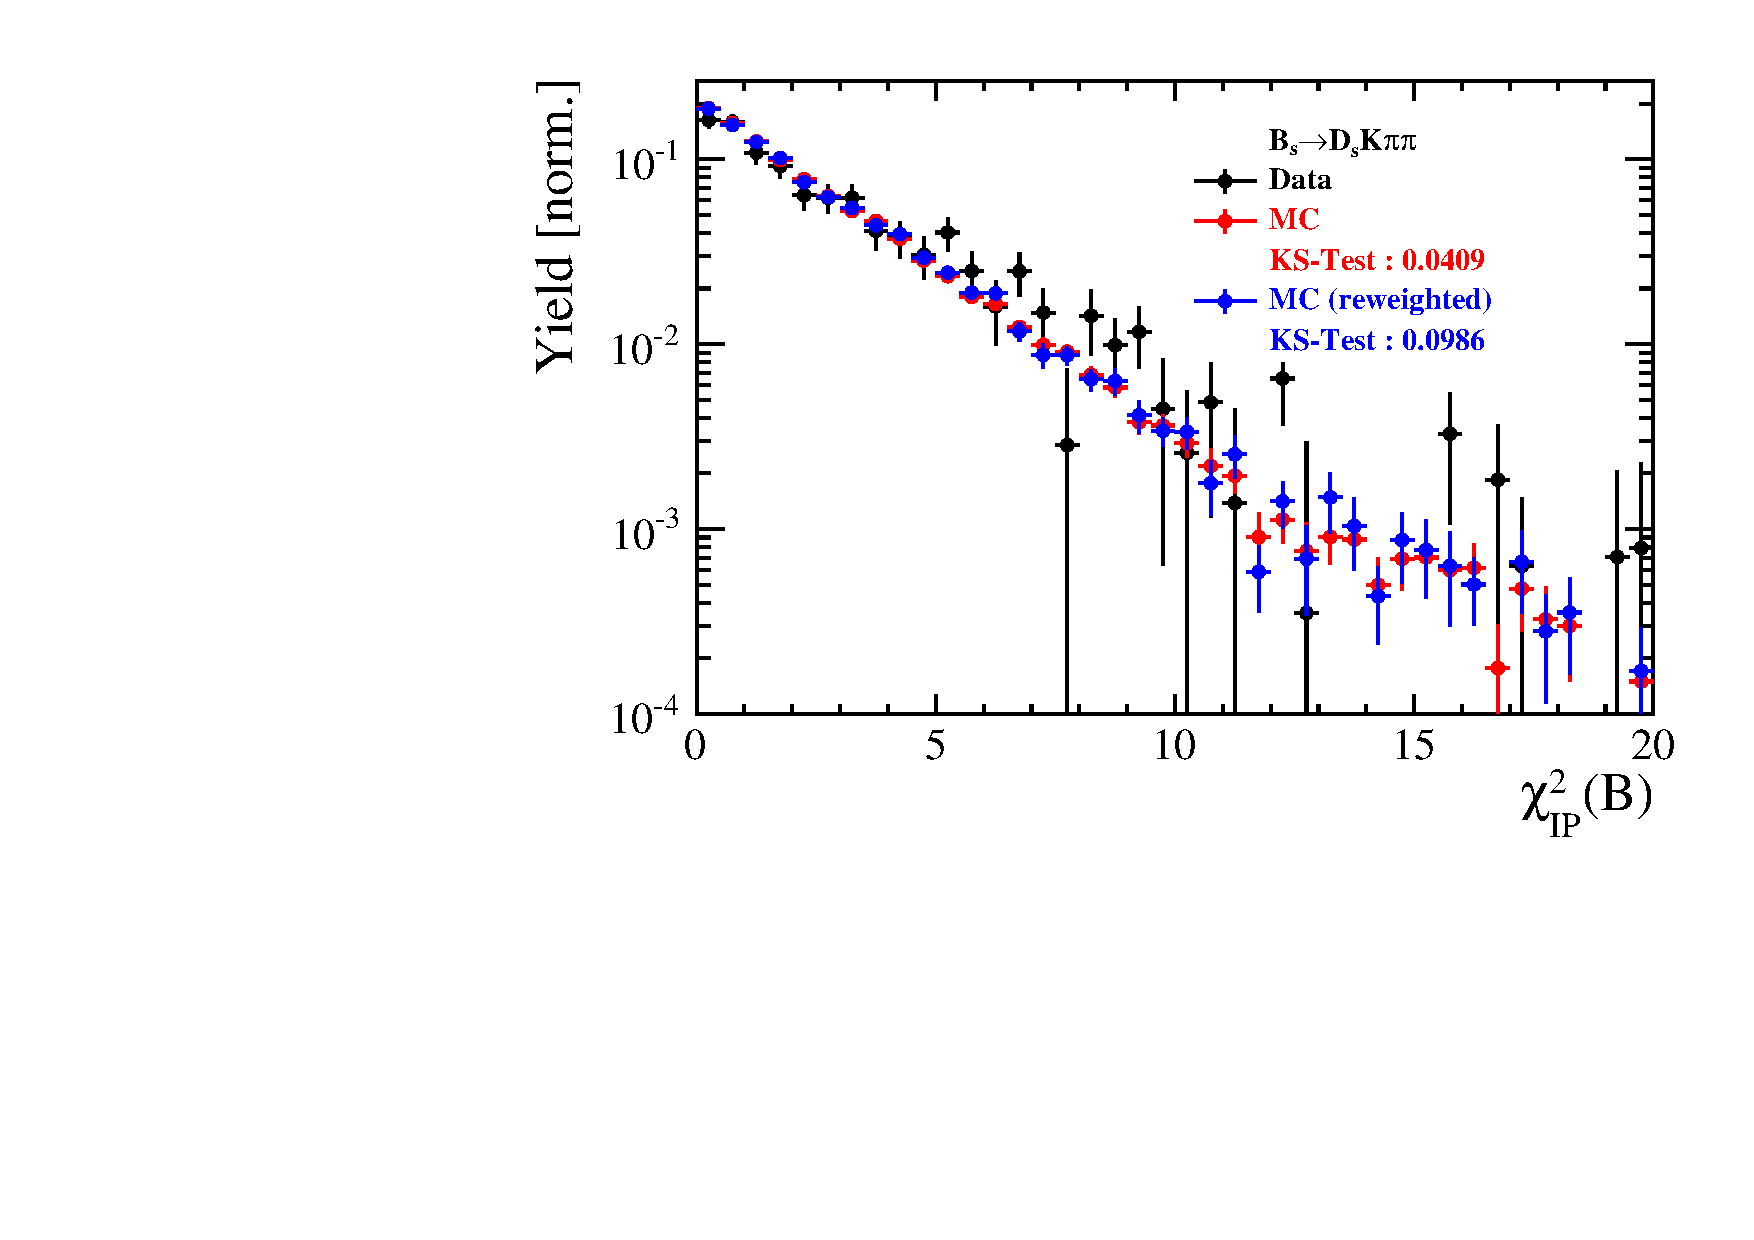
\includegraphics[height=!,width=0.4\textwidth]{figs/dataVsMC/signal_final/combined/Ds2KKpi_1_Bs_IPCHI2_OWNPV.pdf}
%
%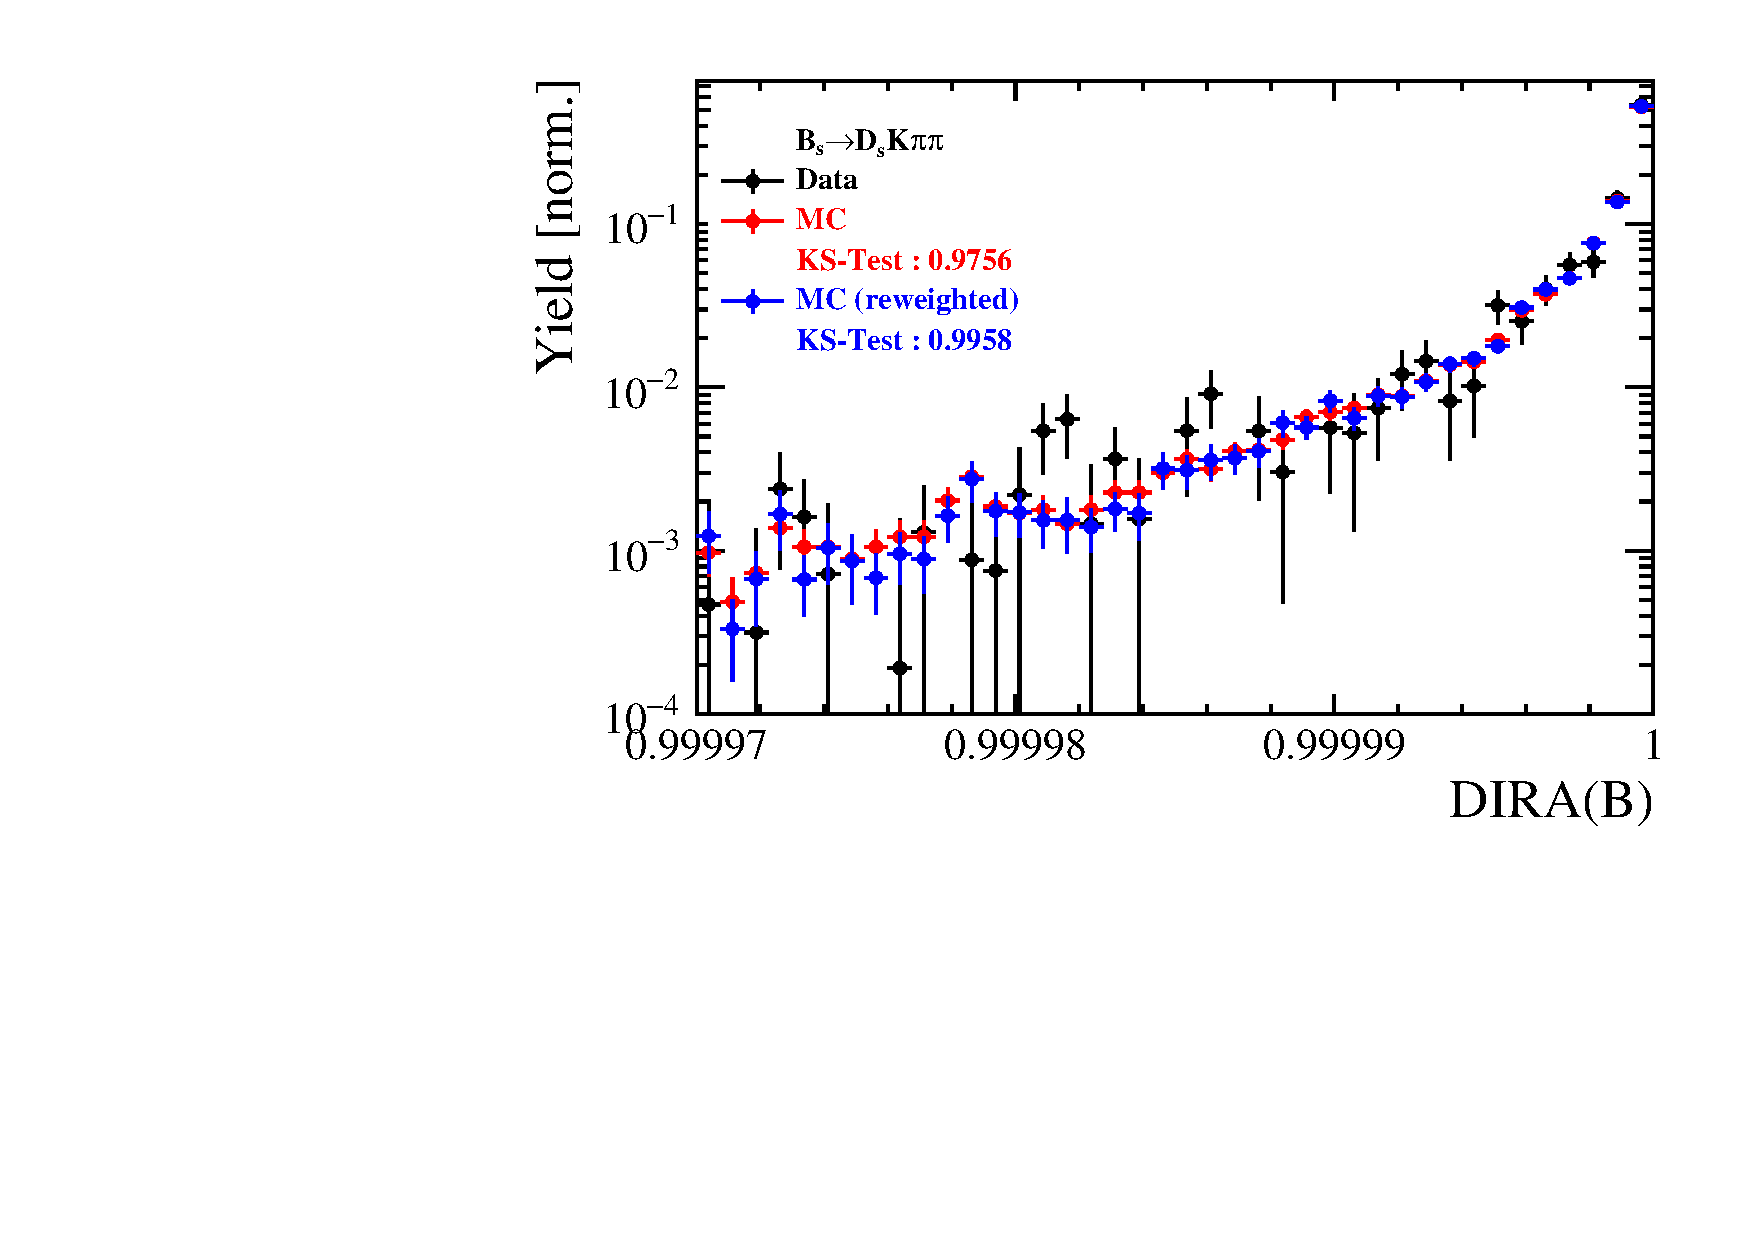
\includegraphics[height=!,width=0.4\textwidth]{figs/dataVsMC/signal_final/combined/Ds2KKpi_1_Bs_DIRA_OWNPV.pdf}
%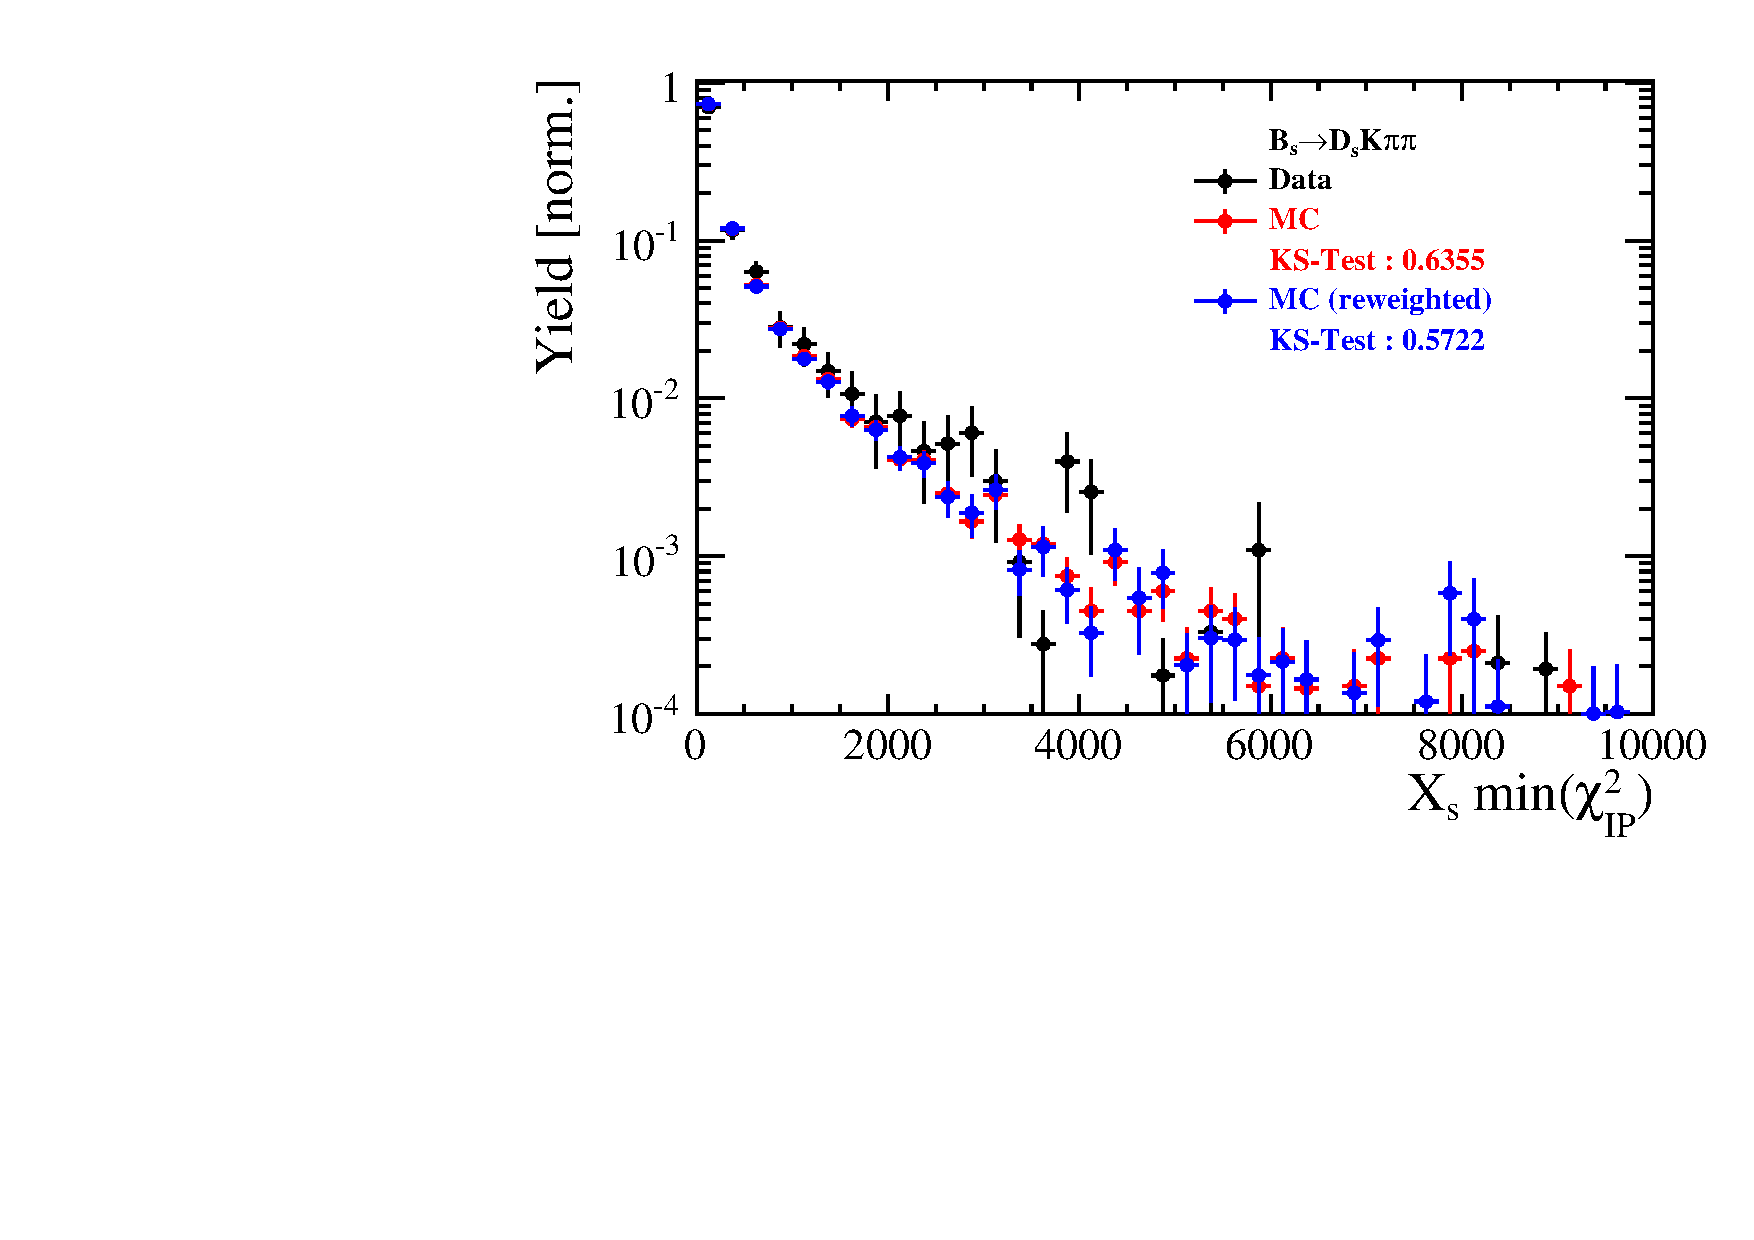
\includegraphics[height=!,width=0.4\textwidth]{figs/dataVsMC/signal_final/combined/Ds2KKpi_1_XsDaughters_min_IPCHI2.pdf}
%
%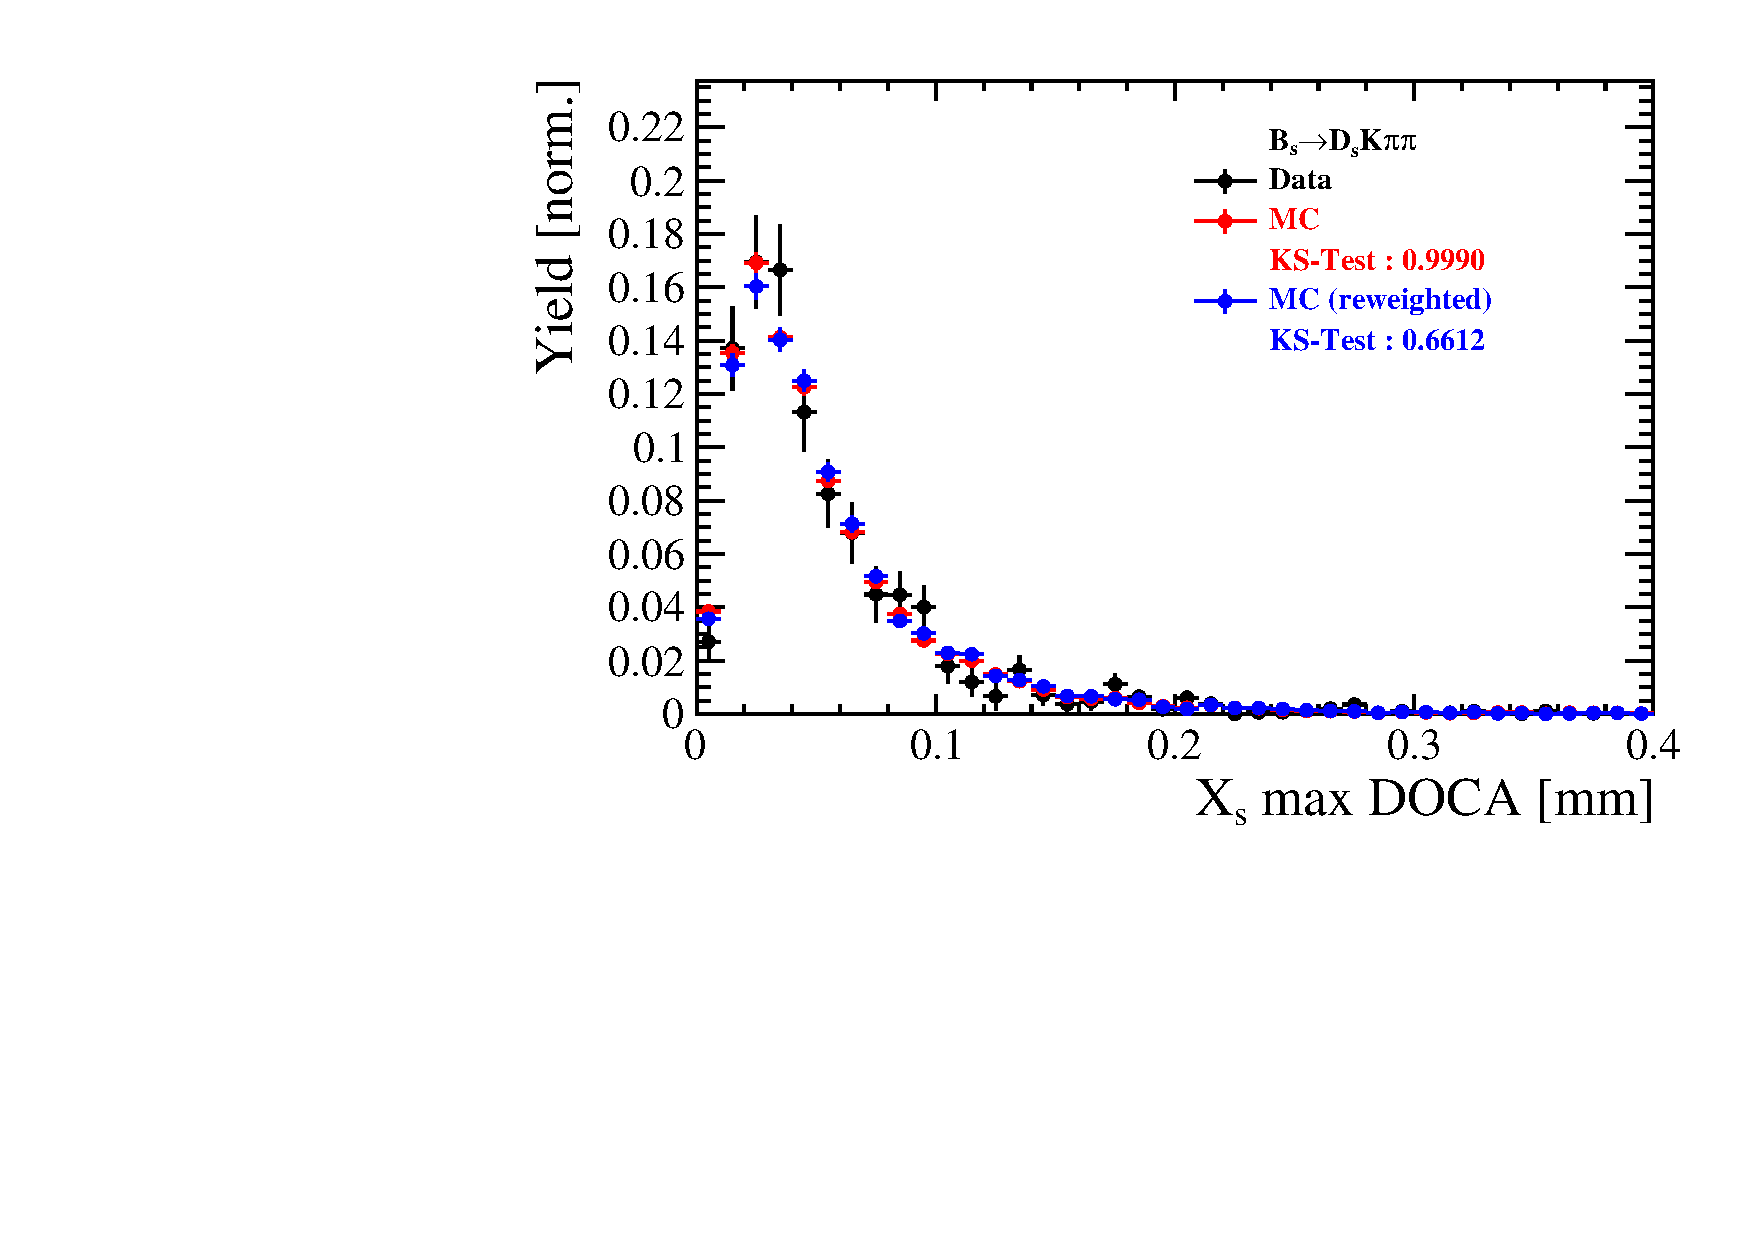
\includegraphics[height=!,width=0.4\textwidth]{figs/dataVsMC/signal_final/combined/Ds2KKpi_1_Xs_max_DOCA.pdf}
%\includegraphics[height=!,width=0.4\textwidth]{figs/dataVsMC/signal_final/combined/Ds2KKpi_1_DsDaughters_min_IPCHI2.pdf}
%
%\includegraphics[height=!,width=0.4\textwidth]{figs/dataVsMC/signal_final/combined/Ds2KKpi_1_Ds_FDCHI2_ORIVX.pdf}
%\includegraphics[height=!,width=0.4\textwidth]{figs/dataVsMC/signal_final/combined/Ds2KKpi_1_maxCos.pdf}
%
%\includegraphics[height=!,width=0.4\textwidth]{figs/dataVsMC/signal_final/combined/Ds2KKpi_1_max_ghostProb.pdf}
%%\includegraphics[height=!,width=0.5\textwidth]{figs/dataVsMC/signal_final/combined/Ds2KKpi_1_Bs_ptasy_1.00.pdf}
%\includegraphics[height=!,width=0.4\textwidth]{figs/dataVsMC/signal_final/combined/Ds2KKpi_1_BDTG_response.pdf}
%
%\caption{Comparison of BDTG input variables and classifier response for $B_s\to D_sK\pi\pi$ decays.}
%\label{fig:}
%\end{figure}
